
\documentclass[a4paper,UKenglish]{lipics-v2018}
%This is a template for producing LIPIcs articles. 
%See lipics-manual.pdf for further information.
%for A4 paper format use option "a4paper", for US-letter use option "letterpaper"
%for british hyphenation rules use option "UKenglish", for american hyphenation rules use option "USenglish"
% for section-numbered lemmas etc., use "numberwithinsect"

\nolinenumbers

\usepackage{microtype}%if unwanted, comment out or use option "draft"

%\graphicspath{{./graphics/}}%helpful if your graphic files are in another directory

\bibliographystyle{plainurl}% the recommnded bibstyle

\title{Typed First-Class Traits}
% \titlerunning{Dummy short title}%optional, please use if title is longer than one line

\author{Xuan Bi}{The University of Hong Kong, Hong Kong, China}{xbi@cs.hku.hk}{}{}%mandatory, please use full name; only 1 author per \author macro; first two parameters are mandatory, other parameters can be empty.

\author{Bruno C. d. S. Oliveira}{The University of Hong Kong, Hong Kong, China}{bruno@cs.hku.hk}{}{}


\authorrunning{X.\,Bi and B.\,C.\,d.\,S.\,Oliveira} %mandatory. First: Use abbreviated first/middle names. Second (only in severe cases): Use first author plus 'et. al.'

\Copyright{Xuan Bi and Bruno C. d. S. Oliveira}%mandatory, please use full first names. LIPIcs license is "CC-BY";  http://creativecommons.org/licenses/by/3.0/


\subjclass{Software and its engineering $\rightarrow$ Object oriented languages}% mandatory: Please choose ACM 2012 classifications from https://www.acm.org/publications/class-2012 or https://dl.acm.org/ccs/ccs_flat.cfm . E.g., cite as "General and reference $\rightarrow$ General literature" or \ccsdesc[100]{General and reference~General literature}.

\keywords{traits, extensible designs}%mandatory

\category{}%optional, e.g. invited paper

\relatedversion{}%optional, e.g. full version hosted on arXiv, HAL, or other respository/website

\supplement{}%optional, e.g. related research data, source code, ... hosted on a repository like zenodo, figshare, GitHub, ...

\funding{Hong Kong Research Grant Council projects number 17210617 and 17258816}%optional, to capture a funding statement, which applies to all authors. Please enter author specific funding statements as fifth argument of the \author macro.

\acknowledgements{We thank the anonymous reviewers for their helpful comments.}%optional

%Editor-only macros:: begin (do not touch as author)%%%%%%%%%%%%%%%%%%%%%%%%%%%%%%%%%%
\EventEditors{Todd Millstein}
\EventNoEds{1}
\EventLongTitle{32nd European Conference on Object-Oriented Programming (ECOOP 2018)}
\EventShortTitle{ECOOP 2018}
\EventAcronym{ECOOP}
\EventYear{2018}
\EventDate{July 16--21, 2018}
\EventLocation{Amsterdam, Netherlands}
\EventLogo{}
\SeriesVolume{109}
\ArticleNo{9} % “New number” (=<article-no>) goes here!%\nolinenumbers %uncomment to disable line numbering
%\hideLIPIcs  %uncomment to remove references to LIPIcs series (logo, DOI, ...), e.g. when preparing a pre-final version to be uploaded to arXiv or another public repository
%%%%%%%%%%%%%%%%%%%%%%%%%%%%%%%%%%%%%%%%%%%%%%%%%%%%%%


% Basics
\usepackage{fixltx2e}
\usepackage{url}
\usepackage{fancyvrb}
\usepackage{mdwlist}  % Miscellaneous list-related commands
\usepackage{xspace}   % Smart spacing
\usepackage{supertabular}
\usepackage{longtable}


% https://www.nesono.com/?q=book/export/html/347
% Package for inserting TODO statements in nice colorful boxes - so that you
% won’t forget to fix/remove them. To add a todo statement, use something like
% \todo{Find better wording here}.
\usepackage{todonotes}

%% Math
\usepackage{amsmath}
\usepackage{amsthm}
\usepackage{amssymb}
\usepackage{bm}       % Bold symbols in maths mode

% http://tex.stackexchange.com/questions/114151/how-do-i-reference-in-appendix-a-theorem-given-in-the-body
\usepackage{thmtools, thm-restate}

%% Theoretical computer science
\usepackage{stmaryrd}
\usepackage{mathtools}  % For "::=" ( \Coloneqq )

%% Font
% \usepackage[euler-digits,euler-hat-accent]{eulervm}


%% Some recommended packages.
\usepackage{booktabs}   %% For formal tables:
                        %% http://ctan.org/pkg/booktabs
\usepackage{subcaption} %% For complex figures with subfigures/subcaptions
                        %% http://ctan.org/pkg/subcaption

% Hyper links
\usepackage{url}
\usepackage{
  nameref,%\nameref
  hyperref,%\autoref
}
\usepackage[capitalise]{cleveref}

% Code highlighting
\usepackage{listings}

\lstset{%
  backgroundcolor=\color{white},
  basicstyle=\small\ttfamily,
  keywordstyle=\sffamily\bfseries,
  captionpos=none,
  columns=flexible,
  lineskip=-1pt,
  keepspaces=true,
  showspaces=false,               % show spaces adding particular underscores
  showstringspaces=false,         % underline spaces within strings
  showtabs=false,                 % show tabs within strings adding particular underscores
  breaklines=true,                % sets automatic line breaking
  breakatwhitespace=true,         % sets if automatic breaks should only happen at whitespace
  escapeinside={(*}{*)},
  literate={->}{{$\rightarrow$}}1 {Top}{{$\top$}}1 {/\\}{{$\Lambda$}}1,
  tabsize=2,
  commentstyle=\color{purple}\ttfamily,
  stringstyle=\color{red}\ttfamily,
  % aboveskip =0pt,
  belowskip =0pt,
  sensitive=false
}

\lstdefinelanguage{sedel}{
  keywords={Void, Class, All, extends, letrec, Int, String, this, inherits, super, type, Trait, override, new, if, then, else, let, in},
  identifierstyle=\color{black},
  morecomment=[l]{--},
  morecomment=[l]{//},
  morestring=[b]",
  xleftmargin  = 3mm,
  morestring=[b]'
}

\lstdefinelanguage{JavaScript}{
  keywords={const, extends, super, class, export, boolean, throw, implements, import, this, typeof, new, true, false, catch, function, return, null, catch, switch, var, if, in, while, do, else, case, break},
  identifierstyle=\color{black},
  comment=[l]{//},
  morecomment=[s]{/*}{*/},
  morestring=[b]',
  xleftmargin  = 3mm,
  morestring=[b]"
}

\lstset{language=sedel}


\usepackage{pifont}

% Revision tools
\usepackage{comment}

% \renewcommand{\paragraph}[1]{\noindent{\bf #1}}

% General
\newcommand{\code}[1]{\texttt {#1}}
\newcommand{\highlight}[1]{\colorbox{GreenYellow}{#1}}

% Math
\newcommand{\im}[1]{\lvert #1 \rvert}

% Constructors
\newcommand{\for}[2]{\forall #1. \, #2}
\newcommand{\lam}[2]{\lambda #1. \, #2}
\newcommand{\app}[2]{#1 \; #2}
\newcommand{\blam}[2]{\Lambda #1. #2}
\newcommand{\tapp}[2]{#1 \; #2}


\newcommand{\arrow}{\rightarrow}

% \newtheorem{theorem}{Theorem}[section]
% \newtheorem{conjecture}{Conjecture}[section]
% \newtheorem{lemma}{Lemma}[section]
% \newtheorem{definition}{Definition}[section]
% \newtheorem{proposition}[theorem]{Proposition}
% \newtheorem{corollary}[theorem]{Corollary}

\newcommand{\mca}{\mathcal{A}}
\newcommand{\mcb}{\mathcal{B}}
\newcommand{\mcc}{\mathcal{C}}
\newcommand{\mcd}{\mathcal{D}}
\newcommand{\mce}{\mathcal{E}}
\newcommand{\mcf}{\mathcal{F}}
\newcommand{\mcg}{\mathcal{G}}
\newcommand{\mch}{\mathcal{H}}
\newcommand{\mci}{\mathcal{I}}
\newcommand{\mcj}{\mathcal{J}}
\newcommand{\mck}{\mathcal{K}}
\newcommand{\mcl}{\mathcal{L}}
\newcommand{\mcm}{\mathcal{M}}
\newcommand{\mcn}{\mathcal{N}}
\newcommand{\mco}{\mathcal{O}}
\newcommand{\mcp}{\mathcal{P}}
\newcommand{\mcq}{\mathcal{Q}}
\newcommand{\mcr}{\mathcal{R}}
\newcommand{\mcs}{\mathcal{S}}
\newcommand{\mct}{\mathcal{T}}
\newcommand{\mcu}{\mathcal{U}}
\newcommand{\mcv}{\mathcal{V}}
\newcommand{\mcw}{\mathcal{W}}
\newcommand{\mcx}{\mathcal{X}}
\newcommand{\mcy}{\mathcal{Y}}
\newcommand{\mcz}{\mathcal{Z}}

\newcommand{\ourlang}{\lambda_{?}}
\newcommand{\ourpolylang}{\lambda_{\rho}^{\it poly}}

\newcommand{\figtwocol}[3]
{\begin{figure}[h!] #3 \caption{#2}\label{#1}\end{figure}}

\newcommand{\myirule}[2]{{\renewcommand{\arraystretch}{1.2}\ba{c} #1
                      \\ \hline #2 \ea}}

\newcommand{\ba}{\begin{array}}
\newcommand{\ea}{\end{array}}
\newcommand{\bda}{\[\ba}
\newcommand{\eda}{\ea\]}

\newcommand{\myset}[1]{\{#1\}}
\newcommand{\relation}[2]{#1:#2}
\newcommand{\myrelation}[2]{#1\!:\!#2}
\newcommand{\To}{\Rightarrow}

\newcommand{\Abs}[2]{\Lambda #1. #2}
\newcommand{\abs}[2]{\lambda #1. #2}
%\newcommand{\ruleabs}[2]{\langle\!|  #2  :  #1 |\!\rangle}
%\newcommand{\ruleabs}[2]{(\!|  #2  :  #1 |\!)}
\newcommand{\ruleabs}[2]{\lambda_? #1. #2}
\newcommand{\ruleapp}[2]{#1 {\bf ~with~} #2}
\newcommand{\iarrow}{\Rightarrow}
\newcommand{\ilambda}{\lambda_{?}}
\newcommand{\with}{{\bf ~with~}}
\newcommand{\query}{?}
\newcommand{\type}{\tau}
\newcommand{\tyint}{{\it Int}}
\newcommand{\tybool}{{\it Bool}}
\newcommand{\tychar}{{\it Char}}
\newcommand{\tystr}{{\it String}}
\newcommand{\tyunit}{()}
\newcommand{\unit}{()}
\newcommand{\btrue}{{\it True}}
\newcommand{\bfalse}{{\it False}}
\newcommand{\Eq}{{\tt Eq}}
\newcommand{\ShowC}{{\tt ShowC}}
\newcommand{\Monad}{{\tt Monad}}
\newcommand{\MonadTrans}{{\tt MonadTrans}}
\newcommand{\GTree}{{\tt GTree}}
\newcommand{\TT}{{\tt \#t}}
\newcommand{\FF}{{\tt \#f}}


\newcommand{\kind}{\kappa}
\newcommand{\rulet}{\rho}
\newcommand{\ruleschr}[3]
{\forall #1. #2 \To #3}
\newcommand{\rulesch}[3]
{\forall \vec{#1}. #2 \To #3}
\newcommand{\ruleset}{\bar{\rulet}}
\newcommand{\rulesetvar}{\ruleset}
\newcommand{\nil}{\varnothing}
\newcommand{\meta}[1]{{\it #1 }}
\newcommand{\finto}{\stackrel{\mathsf{fin}}{\to}}
\newcommand{\rulepgm}{\overline{\relation{\rulet}{v}}}
\newcommand{\rulepgmvar}{\eta}
\newcommand{\grulepgm}[2]{\overline{\relation{#1}{#2}}}
\newcommand{\rulesetexp}{\overline{\relation{e}{\rulet}}}

\newcommand{\FV}     {\meta{fv}}
\newcommand{\FTV}    {\meta{FTV}}
\newcommand{\BV}     {\meta{bv}}
\newcommand{\BTV}    {\meta{BTV}}
\newcommand{\dom}    {\meta{dom}}

\newcommand{\tstate}{\mce}
\newcommand{\rclos}[1]{(#1)}
\newcommand{\lookup}[2]{{#1\langle{#2}\rangle}}
\newcommand{\kenv}{\Phi}
\newcommand{\denv}{\Delta}
\newcommand{\env}{\Delta}
\newcommand{\tenv}{\Gamma}
\newcommand{\eval}{\Downarrow}
\newcommand{\turns}{\vdash}
\newcommand{\vturns}{\vdash_{r}}
\newcommand{\kturns}{\vdash_{k}}
\newcommand{\vtyping}{\models}

%\newcommand{\case}[1]{\----{\bf case}~#1}
\newcommand{\facerule}[1]{{\tt #1}}
\newcommand{\tlabel}[1]{\mbox{(#1)}}

\newcommand{\mylabel}[1]{\tlabel{\facerule{#1}}}

\newcommand{\OpQuery}{\tlabel{\facerule{OpQuery}}}
\newcommand{\OpRule}{\tlabel{\facerule{OpRule}}}
\newcommand{\OpInst}{\tlabel{\facerule{OpInst}}}
\newcommand{\OpRApp}{\tlabel{\facerule{OpRApp}}}
\newcommand{\OpRClos}{\tlabel{\facerule{OpRClos}}}

\newcommand{\TyQuery}{\tlabel{\facerule{Ty-Query}}}
\newcommand{\TyRule}{\tlabel{\facerule{TyRule}}}
\newcommand{\TyInst}{\tlabel{\facerule{TyInst}}}
\newcommand{\TyRApp}{\tlabel{\facerule{TyRApp}}}

\newcommand{\TyRClos}{\tlabel{\facerule{TyRClos}}}
\newcommand{\TyREnv}{\tlabel{\facerule{TyREnv}}}
\newcommand{\TyRPgm}{\tlabel{\facerule{TyRPgm}}}

\newcommand{\RTAbs}{\tlabel{\facerule{RTAbs}}}
\newcommand{\RIAbs}{\tlabel{\facerule{RIAbs}}}
\newcommand{\RSimpl}{\tlabel{\facerule{RSimp}}}

\newcommand{\IDone}{\tlabel{\facerule{IDone}}}
\newcommand{\ITAbs}{\tlabel{\facerule{ITAbs}}}
\newcommand{\IIAbs}{\tlabel{\facerule{IIAbs}}}

\newcommand{\LHere}{\tlabel{\facerule{LHead}}}
\newcommand{\LThere}{\tlabel{\facerule{LTail}}}

\newcommand{\MDone}{\tlabel{\facerule{MDone}}}
\newcommand{\MTAbs}{\tlabel{\facerule{MTAbs}}}
\newcommand{\MIAbs}{\tlabel{\facerule{MIAbs}}}

\newcommand{\TrRTAbs}{\tlabel{\facerule{TrRTAbs}}}
\newcommand{\RRho}{\tlabel{\facerule{RRho}}}
\newcommand{\TrRIAbs}{\tlabel{\facerule{TrRIAbs}}}
\newcommand{\TrRSimpl}{\tlabel{\facerule{TrRSimp}}}

\newcommand{\TrIDone}{\tlabel{\facerule{TrIDone}}}
\newcommand{\TrITAbs}{\tlabel{\facerule{TrITAbs}}}
\newcommand{\TrIIAbs}{\tlabel{\facerule{TrIIAbs}}}

\newcommand{\TrLHere}{\tlabel{\facerule{TrLHead}}}
\newcommand{\TrLThere}{\tlabel{\facerule{TrLTail}}}


\newcommand{\TrInt}{\tlabel{\facerule{TrInt}}}
\newcommand{\TrVar}{\tlabel{\facerule{TrVar}}}
\newcommand{\TrAbs}{\tlabel{\facerule{TrAbs}}}
\newcommand{\TrApp}{\tlabel{\facerule{TrApp}}}
\newcommand{\TrTAbs}{\tlabel{\facerule{TrTAbs}}}
\newcommand{\TrTApp}{\tlabel{\facerule{TrTApp}}}
\newcommand{\TrIAbs}{\tlabel{\facerule{TrIAbs}}}
\newcommand{\TrIApp}{\tlabel{\facerule{TrIApp}}}
\newcommand{\TrQuery}{\tlabel{\facerule{TrQuery}}}

\newcommand{\TermSimpl}{\tlabel{\facerule{TermSimp}}}
\newcommand{\TermTyVar}{\tlabel{\facerule{TermTyVar}}}
\newcommand{\TermInt}{\tlabel{\facerule{TermInt}}}
\newcommand{\TermForall}{\tlabel{\facerule{TermForall}}}
\newcommand{\TermFun}{\tlabel{\facerule{TermFun}}}
\newcommand{\TermRule}{\tlabel{\facerule{TermRule}}}

\newcommand{\ResNil}{\tlabel{\facerule{ResNil}}}
\newcommand{\Res}{\tlabel{\facerule{Res}}}
\newcommand{\SimpleRes}{\tlabel{\facerule{SimpleRes}}}
\newcommand{\RuleRes}{\tlabel{\facerule{RuleRes}}}
\newcommand{\StaRes}{\tlabel{\facerule{TyRes}}}
\newcommand{\DynRes}{\tlabel{\facerule{DynRes}}}

\newcommand{\TrRes}{\tlabel{\facerule{TrRes}}}

\newcommand{\Canon}[1]{\mathsf{canon}(#1)}
\newcommand{\unify}[3]{\mcu_{#3}(#1, #2)}

\newcommand{\KiVar}{\tlabel{\facerule{KiVar}}}
\newcommand{\KiApp}{\tlabel{\facerule{KiApp}}}
\newcommand{\KiForall}{\tlabel{\facerule{KiForall}}}

\newcommand{\err}{{\it err}}

\def\ruleform#1{{\setlength{\fboxrule}{1pt}\fbox{\normalsize $#1$}}}

\newcommand{\Ex}[1]{\[\begin{array}{l}#1\end{array}\]}
\newcommand{\Cmnt}[1]{{\tt #1}}

\newcommand{\subst}[2]{[ #1\!\mapsto\!#2 ]}
\newcommand{\substone}{\subst{\alpha}{\type}}

\newcommand{\leteq}{\overset{{\sf let}}{=}}
\newcommand{\defeq}{\overset{{\sf def}}{=}}

\newcommand{\overlap}{{\sf overlap}}
\newcommand{\nonoverlap}{{\sf nonoverlap}}
\newcommand{\wellformed}{{\sf wellformed}}
\newcommand{\stable}{{\sf stable}}
\newcommand{\coherent}{{\sf coherent}}
\newcommand{\distinct}{{\sf distinct}}
\newcommand{\unrelated}{{\sf unrelated}}
\newcommand{\disjoint}{{\sf distinct}}
\newcommand{\converge}{{\sf converge}}
\newcommand{\welldefined}{{\sf welldefined}}

\newcommand{\distinctrs}{{\sf distinct\_rs}}
\newcommand{\distinctctx}{{\sf distinct\_ctx}}
\newcommand{\distinctwith}{{\sf distinct\_with}}
\newcommand{\unambiguous}{{\sf unambiguous}}

\definecolor{gray}{gray}{0.7}
\definecolor{dark-gray}{gray}{0.4}
\definecolor{light-gray}{gray}{0.8}

%\newcommand{\shade}[1]{\colorbox{gray}{\color{dark-gray} {$#1$}}}
%\newcommand{\shade}[1]{\colorbox{light-gray}{\color{dark-gray} {$#1$}}}
\newcommand{\shade}[1]{\colorbox{light-gray}{\color{black}{$#1$}}}
\newcommand{\hide}[1]{}
\def\myruleform#1{
\setlength{\fboxrule}{0.5pt}\fbox{\normalsize $#1$}
}

\newcommand{\WFIntTy}{\tlabel{\facerule{WF-IntTy}}}
\newcommand{\WFVarTy}{\tlabel{\facerule{WF-VarTy}}}
\newcommand{\WFAbsTy}{\tlabel{\facerule{WF-AbsTy}}}
\newcommand{\WFFunTy}{\tlabel{\facerule{WF-FunTy}}}
\newcommand{\WFRulTy}{\tlabel{\facerule{WF-RulTy}}}

\newcommand{\TyTyAbs}{\tlabel{\facerule{TyTyAbs}}}
\newcommand{\TyTyApp}{\tlabel{\facerule{TyTyApp}}}
\newcommand{\TyUnit}{\tlabel{\facerule{TyUnit}}}
\newcommand{\TyInt}{\tlabel{\facerule{Ty-Int}}}
\newcommand{\TyVar}{\tlabel{\facerule{Ty-Var}}}
\newcommand{\TyIntL}{\tlabel{\facerule{TyIntL}}}
\newcommand{\TyLVar}{\tlabel{\facerule{TyLVar}}}
\newcommand{\TyIVar}{\tlabel{\facerule{TyIVar}}}
\newcommand{\TyRec}{\tlabel{\facerule{TyRec}}}
\newcommand{\TyAbs}{\tlabel{\facerule{Ty-Abs}}}
\newcommand{\TyTAbs}{\tlabel{\facerule{Ty-TAbs}}}
\newcommand{\TyIAbs}{\tlabel{\facerule{Ty-IAbs}}}
\newcommand{\TyApp}{\tlabel{\facerule{Ty-App}}}
\newcommand{\TyTApp}{\tlabel{\facerule{Ty-TApp}}}
\newcommand{\TyIApp}{\tlabel{\facerule{Ty-IApp}}}
\newcommand{\TyLet}{\tlabel{\facerule{TyLet}}}
\newcommand{\TyImp}{\tlabel{\facerule{TyImp}}}
\newcommand{\TyWith}{\tlabel{\facerule{TyWith}}}
\newcommand{\TyAnn}{\tlabel{\facerule{TyAnn}}}

\newcommand{\eqv}{\Longleftrightarrow}

%%% Local Variables: 
%%% mode: latex
%%% TeX-master: "Main"
%%% End: 


% Ott includes
\usepackage{ottalt}
\inputott{ott-rules}
% I prefer rulenames on the right
% \renewcommand\ottaltinferrule[4]{
%   \inferrule*[narrower=0.7,right=#1,#2]
%     {#3}
%     {#4}
% }
\renewcommand\ottaltinferrule[4]{
  \inferrule*[narrower=0.9,lab=#1,#2]
    {#3}
    {#4}
}

% \renewcommand{\ottnt}[1]{#1}
% \renewcommand{\ottmv}[1]{#1}

% \renewcommand{\subparagraph}[1]{\vspace{3pt}\noindent{\bf #1}}

\newcommand{\hll}[2][gray!40]{\colorbox{#1}{#2}}
\newcommand{\hlmath}[2][gray!40]{%
  \colorbox{#1}{$\displaystyle#2$}}


\begin{document}

\maketitle

\begin{abstract}
Many dynamically-typed languages (including JavaScript, Ruby, Python
or Racket) support \emph{first-class classes}, or related concepts
such as first-class traits and/or mixins. In those languages classes
are first-class values and, like any other values, they can be
passed as an argument, or returned from a function. Furthermore
first-class classes support \emph{dynamic inheritance}: i.e. they
can inherit from other classes at \emph{runtime}, enabling
programmers to abstract over the inheritance hierarchy. In contrast,
type system limitations prevent most
statically-typed languages from having first-class classes and
dynamic inheritance.

This paper shows the design of \name: a polymorphic statically-typed
language with \emph{first-class traits}, supporting \emph{dynamic
  inheritance} as well as conventional OO features such as
\emph{dynamic dispatching} and \emph{abstract methods}.  To address
the challenges of type-checking first-class traits, \name employs a type
system based on the recent work on \emph{disjoint
  intersection types} and \emph{disjoint polymorphism}. The novelty of
\name over core disjoint intersection calculi are \emph{source level} features for
practical OO programming, including first-class traits with dynamic inheritance, dynamic
dispatching and abstract methods. Inspired by Cook and Palsberg's work on the
denotational semantics for inheritance, we show how to design a source
language that can be elaborated into Alpuim et al.'s \bname
(a core polymorphic calculus with records supporting disjoint polymorphism).
We illustrate the applicability of \name with several example uses for
first-class traits, and a case study that modularizes programming
language interpreters using a highly modular form of visitors.

\begin{comment}
To allow for \emph{dynamic dispatching} \name
uses

Traits pose additional challenges when compared to
models with first-class classes or mixins, because method conflicts
should be detected \emph{statically}. To enable such dynamic
composition of traits, even when traits are \emph{polymorphic},
SEDEL's type system is based on \emph{disjoint intersection types} and
\emph{disjoint polymorphism}. Inspired by Cook's denotational
semantics of inheritance, this work shows how to develop a source
language.

 While at first such static
detection of conflicts appears to in conflict with dynamic inheritance
(since traits can be plugged


presents a simple language design called \name that supports
\emph{first-class traits}.

essentially  In other words classes are first-class values



Differently from statically typed object

``These untyped languages tend to support flexible mechanisms for class
composition, such as mixins or traits, that allow the programmer to
abstract over inheritance. Fur- thermore, some untyped languages
support a generalization of mixins and traits where classes are
first-class values and thus can inherit from other classes at runtime.''


Object-oriented programming is popular in both statically typed, as
well as dynamically typed languages.

This paper presents \name: a new polymorphic, statically-typed and delegation-based object-oriented
programming language. The design of \name follows Cook et al. motto
of ``\emph{Inheritance is not Subtyping}'' and clearly separates the two notions.
Unlike most previous designs for delegation (or dynamic inheritance)
based languages \name is statically typed;
has an expressive polymorphic type system; and it
supports a powerful form of \emph{conflict-free} multiple dynamic
inheritance mechanism called \emph{dynamically composable traits}.
The design of \name and its type system is based on previous work
on disjoint intersection types and disjoint polymorphism. This
guarantees important \emph{safety} properties, and
ensures a high-degree of programming \emph{flexibility}.
In terms of safety \name's type system provides, not only the usual
type-safety property, but also coherence. The coherence property
ensures that the semantics of \name is unambiguous. In particular
this property is useful to ensure that programs using
multiple dynamic inheritance remain free of conflicts/ambiguities
(even when the types of the object parts being composed are not
statically know).
In terms of flexibility, the polymorphic type system provides
an expressive form of polymorphism and intersection types that
can type-check various delegation-based programs and patterns.
We show how the mechanisms of \name improve extensibility design patterns
such as Extensible Visitors and Object Algebras. Furthermore we show
how the high-level OO mechanisms of \name can be elaborated using
a thin-layer of syntactic sugar into a core calculus with disjoint
intersection types and polymorphism.
\end{comment}
\end{abstract}

%% -- Starting Point --



\section{Introduction}
\label{sec:introduction}

Compositionality is a desirable property in programming
designs. Broadly defined, it is the principle that a
system should be built by composing smaller subsystems. For instance,
in the area of programming languages, compositionality is
a key aspect of \emph{denotational semantics}~\cite{scott1971toward, scott1970outline}, where
the denotation of a program is constructed from the denotations of its parts.
% For example, the semantics for a language of simple arithmetic expressions
% is defined as:
% 
% \[\begin{array}{lcl}
% \llbracket n \rrbracket_{E} & = & n \\
% \llbracket e_1 + e_2 \rrbracket_{E} & = & \llbracket e_1 \rrbracket_E + \llbracket  e_2 \rrbracket_E \\
% \end{array}\]
% 
% \bruno{Replace E by fancier symbol?}
% Here there are two forms of expressions: numeric literals and
% additions. The semantics of a numeric literal is just the numeric
% value denoted by that literal. The semantics of addition is the
% addition of the values denoted by the two subexpressions.
Compositional definitions have many benefits.
One is ease of reasoning: since compositional
definitions are recursively defined over smaller elements they
can typically be reasoned about using induction. Another benefit
is that compositional definitions are easy to extend,
without modifying previous definitions.
% For example, if we also wanted to support multiplication,
% we could simply define an extra case:
% 
% \[\begin{array}{lcl}
% \llbracket e_1 * e_2 \rrbracket_E & = & \llbracket e_1 \rrbracket_E * \llbracket  e_2 \rrbracket_E \\
% \end{array}\]

Programming techniques that support compositional
definitions include:
\emph{shallow embeddings} of
Domain Specific Languages (DSLs)~\cite{DBLP:conf/icfp/GibbonsW14}, \emph{finally
  tagless}~\cite{CARETTE_2009}, \emph{polymorphic embeddings}~\cite{hofer_polymorphic_2008} or
\emph{object algebras}~\cite{oliveira2012extensibility}. These techniques allow us to create
compositional definitions, which are easy to extend without
modifications. Moreover, when modeling semantics, both finally tagless and object algebras
support \emph{multiple interpretations} (or denotations) of
syntax, thus offering a solution to the well-known \emph{Expression Problem}~\cite{wadler1998expression}.
Because of these benefits these techniques have become
popular both in the functional and object-oriented
programming communities.

However, programming languages often only support simple compositional designs
well, while support for more sophisticated compositional designs is lacking.
For instance, once we have multiple interpretations of syntax, we may wish to
compose them. Particularly useful is a \emph{merge} combinator,
which composes two interpretations~\cite{oliveira2012extensibility,
oliveira2013feature, rendel14attributes} to form a new interpretation that,
when executed, returns the results of both interpretations. 

% For example, consider another pretty printing interpretation (or
% semantics) $\llbracket \cdot \rrbracket_P$ for arithmetic expressions, which
% returns the string that denotes the concrete syntax of the
% expression. Using merge we can compose the two interpretations to
% obtain a new interpretation that executes both printing and evaluation:
% \jeremy{Explain what is $E\,\&\,P$?}
% 
% \[\begin{array}{lcl}
% \llbracket \cdot \rrbracket_E \otimes \llbracket \cdot \rrbracket_P & = & \llbracket \cdot \rrbracket_{E\,\&\,P} \\
% \end{array}\]

The merge combinator can be manually defined in existing programming languages,
and be used in combination with techniques such as finally tagless or object
algebras. Moreover variants of the merge combinator are useful to
model more complex combinations
of interpretations. A good example are so-called \emph{dependent} interpretations,
where an interpretation does not depend \emph{only} on itself, but also on 
a different interpretation. These definitions with dependencies are quite
common in practice, and, although they are not orthogonal to the interpretation they
depend on, we would like to model them (and also mutually dependent interpretations)
in a modular and compositional style.

% For example consider the following two
% interpretations ($\llbracket \cdot \rrbracket_{\mathsf{Odd}}$ and
% $\llbracket \cdot \rrbracket_{\mathsf{Even}}$) over Peano-style natural numbers:

% \[\begin{array}{lclclcl}
% \llbracket 0 \rrbracket_{\mathsf{Even}}  & = & \mathsf{True} & ~~~~~~~~~~~~~~~~~~~~ & \llbracket 0 \rrbracket_{\mathsf{Odd}} & = & \mathsf{False} \\
% \llbracket S~e \rrbracket_{\mathsf{Even}} & = & \llbracket e \rrbracket_{\mathsf{Odd}} & ~~ & \llbracket S~e \rrbracket_{\mathsf{Odd}} & = & \llbracket e \rrbracket_{\mathsf{Even}}\\
% \end{array}\]

% \emph{Are these interpretations compositional or not?} Under
% a strict definition of compositionality they are not because
% the interpretation of the parts does not depend \emph{only} on the
% interpretation being defined. Instead both interpretations also depend
% on the other interpretation of the parts. In general,
% definitions with dependencies are quite common in practice.
% In this paper we consider these
% interpretations compositional, and we
% would like to model such dependent (or even mutually dependent)
% interpretations in a modular and compositional style.

Defining the merge combinator in existing
programming languages is verbose and cumbersome, requiring code for every
new kind of syntax. Yet, that code is essentially mechanical and ought to be
automated. 
While using advanced meta-programming techniques enables automating
the merge combinator to a large extent in existing programming
languages~\cite{oliveira2013feature, rendel14attributes}, those techniques have
several problems: error messages can be problematic, type-unsafe reflection
is needed in some approaches~\cite{oliveira2013feature} and
advanced type-level features are required in others~\cite{rendel14attributes}.
An alternative to the merge combinator that supports modular multiple
interpretations and works in OO languages with
support for some form of multiple inheritance and covariant
type-refinement of fields has also been recently
proposed~\cite{zhang19shallow}. 
While this approach is relatively simple, it still
requires a lot of manual boilerplate code for composition of interpretations.

This paper presents a calculus and polymorphic type system with
\emph{(disjoint) intersection types}~\cite{oliveira2016disjoint},
called \fnamee. \fnamee
supports our broader notion of compositional designs, and enables
the development of highly modular and reusable programs. \fnamee
has a built-in merge operator and a powerful subtyping relation that
are used to automate the composition of multiple (possibly dependent)
interpretations. In \fnamee subtyping is coercive and enables the
automatic generation of coercions in a \emph{type-directed} fashion. 
This process is similar to that of other type-directed code generation mechanisms
such as 
\emph{type classes}~\cite{Wadler89typeclasses}, which eliminate 
boilerplate code associated to the \emph{dictionary translation}~\cite{Wadler89typeclasses}.

\fnamee continues a line of
research on disjoint intersection types.
 Previous work on
\emph{disjoint polymorphism} (the \fname calculus)~\cite{alpuimdisjoint} studied the
combination of parametric polymorphism and disjoint intersection
types, but its subtyping relation does not support
BCD-style distributivity rules~\cite{Barendregt_1983} and the type system
also prevents unrestricted intersections~\cite{dunfield2014elaborating}. More recently the \name
calculus (or \namee)~\cite{bi_et_al:LIPIcs:2018:9227} introduced a system with \emph{disjoint
  intersection types} and BCD-style distributivity rules, but did not
account for parametric polymorphism. \fnamee is unique in that it
combines all three features in a single calculus:
\emph{disjoint intersection types} and a \emph{merge operator};
\emph{parametric (disjoint) polymorphism}; and a BCD-style subtyping
relation with \emph{distributivity rules}. The three features together
allow us to improve upon the finally tagless and object
algebra approaches and support advanced compositional designs.
Moreover previous work on disjoint intersection types has shown 
various other applications that are also possible in \fnamee, including: \emph{first-class
  traits} and \emph{dynamic inheritance}~\cite{bi_et_al:LIPIcs:2018:9214}, \emph{extensible records} and \emph{dynamic
  mixins}~\cite{alpuimdisjoint}, and \emph{nested composition} and \emph{family polymorphism}~\cite{bi_et_al:LIPIcs:2018:9227}. 


Unfortunately the combination of the three features has non-trivial
complications. The main technical challenge (like for most other
calculi with disjoint intersection types) is the proof of coherence
for \fnamee. Because of the presence of BCD-style distributivity
rules, our coherence proof is based on the recent approach employed in
\namee~\cite{bi_et_al:LIPIcs:2018:9227}, which uses a
\emph{heterogeneous} logical relation called \emph{canonicity}. To account for polymorphism,
which \namee's canonicity does not support, we originally wanted
to incorporate the relevant parts of System~F's logical relation~\cite{reynolds1983types}.
However, due to a mismatch between the two relations, this did not work. The
parametricity relation has been carefully set up with a delayed type
substitution to avoid ill-foundedness due to its impredicative polymorphism.
Unfortunately, canonicity is a heterogeneous relation and needs to account for
cases that cannot be expressed with the delayed substitution setup of the
homogeneous parametricity relation. Therefore, to handle those heterogeneous
cases, we resorted to immediate substitutions and 
% restricted \fnamee to
\emph{predicative instantiations}.
%other
%measures to avoid the ill-foundedness of impredicative instantiation.
%We have settled on restricting \fnamee to \emph{predicative polymorphism} to
%keep the coherence proof manageable. 
We do not believe that predicativity is a severe restriction in practice, since many source
languages (e.g., those based on the Hindley-Milner type system like Haskell and
OCaml) are themselves predicative and do not require the full generality of an
impredicative core language. Should impredicative instantiation be required,
we expect that step-indexing~\cite{ahmed2006step} can be used to recover well-foundedness, though
at the cost of a much more complicated coherence proof.

The formalization and metatheory of \fnamee are a significant advance over that of
\fname. Besides the support for distributive subtyping, \fnamee removes 
several restrictions imposed by the syntactic coherence
proof in \fname. In particular \fnamee supports unrestricted
intersections, which are forbidden in \fname. Unrestricted
intersections enable, for example, encoding certain forms of 
bounded quantification~\cite{pierce1991programming}.
Moreover the new proof method is more robust
with respect to language extensions. For instance, \fnamee supports the bottom
type without significant complications in the proofs, while it was a challenging
open problem in \fname.
A final interesting aspect is that \fnamee's type-checking is decidable. In the
design space of languages with polymorphism and subtyping, similar mechanisms
have been known to lead to undecidability. Pierce's seminal paper
``\emph{Bounded quantification is undecidable}''~\cite{pierce1994bounded} shows
that the contravariant subtyping rule for bounded quantification in
\fsub leads to undecidability of subtyping.  In \fnamee the
contravariant rule for disjoint quantification retains decidability. 
Since with unrestricted intersections \fnamee can express several
use cases of bounded quantification, \fnamee could be an interesting and
decidable alternative to \fsub.

\begin{comment}
Besides coherence, we show
several other important meta-theoretical results, such as type-safety, 
sound and complete algorithmic subtyping, and
decidability of the type system. Remarkably, unlike 
\fsub's \emph{bounded polymorphism}, disjoint polymorphism
in \fnamee supports decidable type-checking.
\end{comment}

In summary the contributions of this paper are:
\begin{itemize}

\item {\bf The \fnamee calculus,} which is the first calculus to combine 
disjoint intersection types, BCD-style distributive subtyping and 
disjoint polymorphism. We show several meta-theoretical results, such as \emph{type-safety}, \emph{sound and complete algorithmic subtyping},
\emph{coherence} and \emph{decidability} of the type system.
\fnamee includes the \emph{bottom type}, which was considered to be a
significant challenge in previous work on disjoint polymorphism~\cite{alpuimdisjoint}.

\item {\bf An extension of the canonicity relation with polymorphism,}
  which enables the proof of coherence of \fnamee. We show that the ideas of
  System F's \emph{parametricity} cannot be ported to
  \fnamee. To overcome the problem we use a technique based on
  immediate substitutions and a predicativity restriction.

% \item {\bf Disjoint intersection types in the presence of bottom:}
%   Our calculus includes the bottom type, which was considered to be a
% significant challenge in previous work on disjoint polymorphism~\cite{alpuimdisjoint}.

\item {\bf Improved compositional designs:} We show that \fnamee's combination of features
enables improved
compositional programming designs and supports automated composition
of interpretations in programming techniques like object algebras and
finally tagless.

\item {\bf Implementation and proofs:} All of the metatheory
  of this paper, except some manual proofs of decidability, has been
  mechanically formalized in Coq. Furthermore, \fnamee is
  implemented and all code presented in the paper is available. The
  implementation, Coq proofs and extended version with appendices can be found in
  \url{https://github.com/bixuanzju/ESOP2019-artifact}.

\end{itemize}

% \bruno{
% Still need to figure out how to integrate row types in the intro story
% Furthermore, we provide a detailed
% comparison between \emph{distributive disjoint polymorphism} and
% \emph{row types}.
% }

% Compositionality is a desirable property in programming
% designs. Broadly defined, compositionality is the principle that a
% system should be built by composing smaller subsystems.
% In the area of programming languages compositionality is
% a key aspect of \emph{denotational semantics}~\cite{scott1971toward, scott1970outline}, where
% the denotation of a program is constructed from denotations of its parts.
% For example, the semantics for a language of simple arithmetic expressions
% is defined as:
% 
% \[\begin{array}{lcl}
% \llbracket n \rrbracket_{E} & = & n \\
% \llbracket e_1 + e_2 \rrbracket_{E} & = & \llbracket e_1 \rrbracket_E + \llbracket  e_2 \rrbracket_E \\
% \end{array}\]
% 
% \bruno{Replace E by fancier symbol?}
% Here there are two forms of expressions: numeric literals and
% additions. The semantics of a numeric literal is just the numeric
% value denoted by that literal. The semantics of addition is the
% addition of the values denoted by the two subexpressions.
% Compositional definitions have many benefits.
% One is ease of reasoning: since compositional
% definitions are recursively defined over smaller elements they
% can typically be reasoned about using induction. Another benefit
% of compositional definitions is that they are easy to extend,
% without modifying previous definitions.
% For example, if we also wanted to support multiplication,
% we could simply define an extra case:
% 
% \[\begin{array}{lcl}
% \llbracket e_1 * e_2 \rrbracket_E & = & \llbracket e_1 \rrbracket_E * \llbracket  e_2 \rrbracket_E \\
% \end{array}\]
% 
% Programming techniques that support compositional
% definitions include:
% \emph{shallow embeddings} of
% Domain Specific Languages (DSLs)~\cite{DBLP:conf/icfp/GibbonsW14}, \emph{finally
%   tagless}~\cite{CARETTE_2009}, \emph{polymorphic embeddings}~\cite{} or
% \emph{object algebras}~\cite{oliveira2012extensibility}. All those techniques allow us to easily create
% compositional definitions, which are easy to extend without
% modifications. Moreover both finally tagless and object algebras
% support \emph{multiple interpretations} (or denotations) of
% the syntax, thus offering a solution to the infamous \emph{Expression Problem}~\cite{wadler1998expression}.
% Because of these benefits they have become
% popular both in the functional and object-oriented
% programming communities.
% 
% However, programming languages often only support simple
% compositional designs well, while language support for more sophisticated
% compositional designs is lacking. Once we have multiple
% interpretations of syntax, then we may wish to compose those
% interpretations. In particular, when multiple interpretations exist, a useful operation
% is a \emph{merge} combinator ($\otimes$) that composes two
% interpretations~\cite{oliveira2012extensibility, oliveira2013feature, rendel14attributes}, forming a
% new interpretation that, when executed, returns the results of both
% interpretations. For example, consider another pretty printing interpretation (or
% semantics) $\llbracket \cdot \rrbracket_P$ for arithmetic expressions, which
% returns the string that denotes the concrete syntax of the
% expression. Using merge we can compose the two interpretations to
% obtain a new interpretation that executes both printing and evaluation:
% \jeremy{Explain what is $E\,\&\,P$?}
% 
% \[\begin{array}{lcl}
% \llbracket \cdot \rrbracket_E \otimes \llbracket \cdot \rrbracket_P & = & \llbracket \cdot \rrbracket_{E\,\&\,P} \\
% \end{array}\]
% 
% Such merge combinator can be manually defined in existing programming 
% The merge combinator can be manually defined in existing programming
% languages, and be used in combination with techniques such as finally
% tagless or object algebras. Furthermore variants of the
% merge combinator can help express more complex combinations of multiple
% interpretations. For example consider the following two
% interpretations ($\llbracket \cdot \rrbracket_{\mathsf{Odd}}$ and
% $\llbracket \cdot \rrbracket_{\mathsf{Even}}$) over Peano-style natural numbers:
% 
% \[\begin{array}{lclclcl}
% \llbracket 0 \rrbracket_{\mathsf{Even}}  & = & \mathsf{True} & ~~~~~~~~~~~~~~~~~~~~ & \llbracket 0 \rrbracket_{\mathsf{Odd}} & = & \mathsf{False} \\
% \llbracket S~e \rrbracket_{\mathsf{Even}} & = & \llbracket e \rrbracket_{\mathsf{Odd}} & ~~ & \llbracket S~e \rrbracket_{\mathsf{Odd}} & = & \llbracket e \rrbracket_{\mathsf{Even}}\\
% \end{array}\]
% 
% \emph{Are these interpretations compositional or not?} Under
% a strict definition of compositionality they are not because
% the interpretation of the parts does not depend \emph{only} on the
% interpretation being defined. Instead both interpretations also depend
% on the other interpretation of the parts. In general,
% definitions with dependencies are quite common in practice.
% In this paper we consider these
% interpretations compositional, and we
% would like to model such dependent (or even mutually dependent)
% interpretations in a modular and compositional style.
% 
% However defining the merge combinator in existing programming
% languages is verbose and cumbersome, and requires code for every new
% kind of syntax. Yet, that code is essentially mechanical and
% ought to be automated. While using advanced meta-programming
% techniques enables automating the merge combinator to a large extent
% in existing programming languages~\cite{oliveira2013feature, rendel14attributes}, those techniques have
% several problems. For example, error messages can be problematic, some
% techniques rely on type-unsafe reflection, while other techniques
% require highly advanced type-level features.
% 
% This paper presents a calculus and polymorphic type system with
% \emph{(disjoint) intersection types}~\cite{oliveira2016disjoint}, called \fnamee, that
% supports our broader notion of compositional designs, and enables
% the development of highly modular and reusable programs. \fnamee
% has a built-in merge operator and a powerful subtyping relation that
% are used to automate the composition of multiple interpretations
% (including dependent interpretations). \fnamee continues a line of
% research on disjoint intersection types. Previous work on
% \emph{disjoint polymorphism} (the \fname calculus) studied the
% combination between parametric polymorphism and disjoint intersection
% types, but the subtyping relation did not support
% BCD-style distributivity rules~\cite{Barendregt_1983}. More recently the \name
% calculus (or \namee) studied a system with \emph{disjoint
%   intersection types} and BCD-style distributivity rules, but did not
% account for parametric polymorphism. \fnamee is unique in that it
% allows the combination of three useful features in a single calculus:
% \emph{disjoint intersection types} and a \emph{merge operator};
% \emph{parametric (disjoint) polymorphism}; and a BCD-style subtyping
% relation with \emph{distributivity rules}. All three features are
% necessary to use improved versions of finally tagless or object
% algebras that support improved compositional designs.
% 
% Unfortunatelly the combination of the three features has non-trivial
% complications. The main technical challenge (as often is the case for
% calculi with disjoint intersection types) is the proof of coherence
% for \fnamee. Because of the presence BCD-style distributivity
% rules, the proof of coherence is based on the approach using a
% \emph{heterogeneous} logical relation employed in
% \namee~\cite{bi_et_al:LIPIcs:2018:9227}. However the logical relation in
% \namee, which we call here \emph{canonicity}, does not
% account for polymorphism. To account for polymorphism we originally
% expected to simply borrow ideas from \emph{parametricity}~\cite{reynolds1983types} in
% System F~\cite{reynolds1974towards} and adapt them to fit with the canonicity relation.
% However, this did not work. The problem is partly due to the fact that
% canonicity (unlike parametricity) is an heterogenous relation and
% needs to account for heterogeneous cases that are not considered in an
% homogeneous relation such as parametricity. Those heterogeneous cases, combined
% with \emph{impredicative polymorphism}, resulted in an ill-founded logical
% relation. Fortunatelly it turns out that
% restricting the calculus to \emph{predicative polymorphism} and using
% an approach based on substitutions is
% sufficient to recover a well-founded canonicity relation.
% Therefore we
% adopted this approach in \fnamee.
% We do not view
% the predicativity restriction as being very severe in practice, since many
% practical languages have such restriction as well. For example languages based
% on Hindley-Milner style type systems (such as Haskell, OCaml or ML)
% \ningning{it's hard to say this is true. When we say Hindley-Milner type system,
%   or Haskell, we are referring to the source language. However, the core
%   language for, for example Haskell, which is System FC, is impredicative.
%   \fnamee is more close to a core language (which usually has explicit type
%   abstractions/applications). In this sense it's unfair to compare it with other
%   source languages.} all use predicative polymorphism. Furthermore with the
% predicativity restriction, the canonicity relation and corresponding proofs
% remain relatively simple and do not require emplying more complex approaches
% such as \emph{step-indexed logical relations}. \ningning{we should emphasize
%   that predicativity is not a restriction, rather it's choice we made in order
%   to prove coherence in Coq. Step-indexed logical relation might work for
%   impredicativity; it's just we don't know.}
% 
% In summary the contributions of this paper are:
% 
% \begin{itemize}
% 
% \item {\bf The \fnamee calculus,} which integrates disjoint intersection types,
%     distributivity and disjoint polymorphism. \fnamee
%     is the first calculus puts all three features together. The
%     combination is non-trivial, expecially with respect to the
%     coherence proof.
% 
% \bruno{improve text}
% \item {\bf The canonicity logical relation,} which enables the proof
%     of coherence of \fnamee. We show that the ideas of
%   System F's \emph{parametricity} cannot be ported to
%   \fnamee. To overcome the problem we develop a canonicity
%   relation that enables a proof of coherence.
% 
% \item {\bf Disjoint intersection types in the presence of bottom:}
%   Our calculus includes a bottom type, which was considered to be a
% significant challenge in previous work.
% 
% \item {\bf Improved compositional designs:} We show how \fnamee has all the
% features that enable improved
% compositional programming designs and support automated composition
% of interpretations in programming techniques like object algebras and
% finally tagless.
% 
% \item {\bf Implementation and proofs:} All proofs
% (including type-safety, coherence and decidability of the type system)
% are proved in the Coq theorem prover. Furthermore \sedel \ningning{where comes the name \sedel?} and
% \fnamee are implemented and all code presented in the paper is
% available. The implementation, proofs and examples can be found in:
% 
% \url{MISSING}
% 
% \end{itemize}
% 
% \bruno{
% Still need to figure out how to integrate row types in the intro story
% Furthermore, we provide a detailed
% comparison between \emph{distributive disjoint polymorphism} and
% \emph{row types}.
% }

% Local Variables:
% org-ref-default-bibliography: "../paper.bib"
% End:



\section{Overview}
\label{sec:overview}

This section aims at introducing first-class classes and traits, their possible
uses and applications, as well as the typing challenges that arise
from their use.
We start by describing a hypothetical JavaScript library for text editing
widgets, inspired and adapted from Racket's GUI
toolkit~\cite{DBLP:conf/oopsla/TakikawaSDTF12}. The example is illustrative of
typical uses of dynamic inheritance/composition, and also the typing challenges
in the presence of first-class classes/traits. Without diving into
technical details, we then give the corresponding typed version in
\name, and informally presents its salient features.

\subsection{First-Class Classes in JavaScript}

A class construct was officially added to JavaScript in the ECMAScript
2015 Language Specification~\cite{EcmaScript:15}. One purpose of
adding classes to JavaScript was to support a construct that is more
familiar to programmers who come from mainstream class-based languages,
such as Java or C++. However classes in JavaScript are
\emph{first-class} and support functionality not easily mimicked in
statically-typed class-based languages.

\subparagraph{Conventional Classes.}
Before diving into the more advanced features of JavaScript classes, we first
review the more conventional class declarations supported in JavaScript as well
as many other languages. Even for conventional classes there are some
interesting points to note about JavaScript that will be important when we move
into a typed setting. An example of a JavaScript class declaration is:
\begin{lstlisting}[language=JavaScript]
class Editor {
  onKey(key) { return "Pressing " + key; }
  doCut()    { return this.onKey("C-x") + " for cutting text"; }
  showHelp() { return "Version: " + this.version() + " Basic usage..."; }
};
\end{lstlisting}
This form of class definition is standard and very similar to declarations in
class-based languages (for example Java). The \lstinline{Editor} class
defines three methods: \lstinline{onKey} for handling key events,
\lstinline{doCut} for cutting text and \lstinline{showHelp} for displaying help
message. For the purpose of demonstration, we elide the actual implementation,
and replace it with plain messages.

We wish to bring the readers' attention to two points in the above class.
Firstly, note that the \lstinline{doCut} method is defined in terms of the
\lstinline{onKey} method via the keyword
\lstinline[language=JavaScript]{this}. In other words the call to
\lstinline{onKey} is enabled by the \emph{self} reference and is
\emph{dynamically dispatched} (i.e., the particular implementation of
\lstinline{onKey} will only be determined when the class or subclass
is instantiated). % Typically an
% OO programmer seeing this definition would expect the \lstinline{doCut} method
% to call the \lstinline{onKey} method of a subclass of \lstinline{Editor}, even though
% the subclass does not exist when the superclass \lstinline{Editor} is being
% defined.
Secondly, notice that there is no definition of
the \lstinline{version} method in the class body, but such method is used inside the
\lstinline{showHelp} method. In a untyped language, such as JavaScript, using
undefined methods is error prone -- accidentally instantiating \lstinline{Editor}
and then calling \lstinline{showHelp} will cause a runtime error!
Statically-typed languages usually provide some means to protect us from this
situation. For example, in Java, we would need an \textit{abstract} \lstinline{version}
method, which effectively makes \lstinline{Editor} an abstract class and
prevents it from being instantiated. As we will see, \name's treatment of
abstract methods is quite different from mainstream languages. In fact, \name
has a unified (typing) mechanism for dealing with both dynamic dispatch and abstract
methods. We will describe \name's mechanism for dealing with both features and
justify our design in \cref{sec:traits}.

% A couple of things worth pointing out in the above code snippet: (1) the class
% \lstinline{Editor} has no definition of the method
% \lstinline{version}, but such method
% is used in the body of the method \lstinline{showHelp}. In a strongly-typed OO
% language, such as Java, we would need to define an abstract method for
% \lstinline{version}. (2) The \lstinline{Editor} class requires
% \emph{dynamic dispatching}.
%  In the body of the method \lstinline{doCut} we invoke
% the method \lstinline{onKey} defined in the same class through the keyword
% \lstinline[language=JavaScript]{this}. This has the implication that when a
% subclass of \lstinline{Editor} overrides the method \lstinline{onKey}, a call to
% \lstinline{doCut} should invoke \lstinline{onKey} defined in the subclass
% instead of the original one.\bruno{punchline?}
%As we will see later, the type system of \name correctly handles it.

\subparagraph{First-Class Classes and Class Expressions.}
Another way to define a class in JavaScript is via a \emph{class expression}. This is where the class
model in JavaScript is very different from the traditional class model found in
many mainstream OO languages, such as Java, where classes are second-class
(static) entities. JavaScript embraces a dynamic class model that treats classes
as \emph{first-class} expressions: a function can take classes as arguments,
or return them as a result. First-class classes enable programmers to
abstract over patterns in the class hierarchy and to experiment with new forms of OOP
such as mixins and traits. In particular, mixins become programmer-defined
constructs. We illustrate this by presenting a simple mixin that adds
spell checking to an editor:
\begin{lstlisting}[language=JavaScript]
const spellMixin = Base => {
  return class extends Base {
    check()    { return super.onKey("C-c") + " for spell checking"; }
    onKey(key) { return "Process " + key + " on spell editor"; }
  }
};
\end{lstlisting}
In JavaScript, a mixin is simply a function with a superclass as input and a
subclass extending that superclass as an output. Concretely, \lstinline{spellMixin}
adds a method \lstinline{check} for spell checking. It also provides
a method \lstinline{onKey}.
The function \lstinline{spellMixin} shows the typical use of what we call \emph{dynamic inheritance}.
Note that \lstinline{Base}, which is supposed to be a superclass being inherited, is \emph{parameterized}.
Therefore \lstinline{spellMixin} can be applied to any base class at
\emph{runtime}. This is impossible to do, in a type-safe way, in
conventional statically-typed class-based languages like Java or
C++.\footnote{With C++ templates, it is possible to
  implement a so-called mixin pattern~\cite{DBLP:conf/gcse/SmaragdakisB00}, which enables extending
a parameterized class. However C++ templates defer type-checking until
instantiation, and such pattern still does not allow selection of the
base class at runtime (only at up to class instantiation time).}

It is noteworthy that not all applications of \lstinline{spellMixin} to base
classes are successful. Notice the use of the \lstinline{super} keyword in the
\lstinline{check} method. If the base class does not implement the
\lstinline{onKey} method, then mixin application fails with a runtime error. In
a typed setting, a type system must express this requirement (i.e., the presence of
the \lstinline{onKey} method) on the (statically unknown) base class that is
being inherited.


% The class expression inside the function body has no
% definition of the method \lstinline{version}, but which is used in the body of
% the method \lstinline{showHelp}. In a statically-typed OO language, such as Java,
% we would need an \emph{abstract method} for
% \lstinline{version}.


We invite the readers to pause for a while and think about what the type of
\lstinline{spellMixin} would look like. Clearly our type system should be
flexible enough to express this kind of dynamic pattern of composition in order
to accommodate mixins (or traits), but also not too lenient to allow any
composition.


\subparagraph{Mixin Composition and Conflicts.}
The real power of mixins is that \lstinline{spellMixin}'s functionality is not
tied to a particular class hierarchy and is composable with other features. For
example, we can define another mixin that adds simple modal editing -- as in Vim
-- to an arbitrary editor:
\begin{lstlisting}[language=JavaScript]
const modalMixin = Base => {
  return class extends Base {
    constructor() {
      super();
      this.mode = "command";
    }
    toggleMode() { return "toggle succeeded"; }
    onKey(key)   { return "Process " + key + " on modal editor"; }
  };
};
\end{lstlisting}
\lstinline{modalMixin} adds a \lstinline{mode} field that controls which
keybindings are active, initially set to the command mode, and a method
\lstinline{toggleMode} that is used to switch between modes. It also provides a method \lstinline{onKey}.

Now we can compose \lstinline{spellMixin} with \lstinline{modalMixin} to produce
a combination of functionality, mimicking some form of multiple inheritance:
\begin{lstlisting}[language=JavaScript]
class IDEEditor extends modalMixin(spellMixin(Editor)) {
  version() { return 0.2; }
}
\end{lstlisting}
The class \lstinline{IDEEditor} extends the base class \lstinline{Editor} with
modal editing and spell checking capabilities. It also defines the missing
\lstinline{version} method.

At first glance, \lstinline{IDEEditor} looks quite fine, but it has a subtle
issue. Recall that two mixins \lstinline{modalMixin} and \lstinline{spellMixin}
both provide a method \lstinline{onKey}, and the \lstinline{Editor} class also
defines an \lstinline{onKey} method of its own. Now we have a name clash. A
question arises as to which one gets picked inside the \lstinline{IDEEditor}
class. A typical mixin model resolves this issue by looking at the order of mixin applications. Mixins appearing later in the order
overrides \emph{all} the identically named methods of earlier mixins. So in our
case, \lstinline{onKey} in \lstinline{modalMixin} gets picked. If we
change the order of application to \lstinline{spellMixin(modalMixin(Editor))},
then \lstinline{onKey} in \lstinline{spellMixin} is inherited.

\subparagraph{Problem of Mixin Composition.}
From the above discussion, we can see that mixin are composed linearly: all the
mixins used by a class must be applied one at a time. However, when we wish to
resolve conflicts by selecting features from different mixins, we may not be
able to find a suitable order. For example, when we compose the two mixins to
make the class \lstinline{IDEEditor}, we can choose which of them comes first,
but in either order, \lstinline{IDEEditor} cannot access to the \lstinline{onKey}
method in the \lstinline{Editor} class.

\subparagraph{Trait Model.}
Because of the total ordering and the limited means for resolving conflicts imposed by the mixin model,
researchers have proposed a simple compositional model called
traits~\cite{scharli2003traits, Ducasse_2006}. Traits are lightweight entities and serve as
the primitive units of code reuse. Among others, the key difference from
mixins is that the order of trait composition is irrelevant, and conflicting
methods must be resolved \emph{explicitly}. This gives programmers
fine-grained control, when conflicts arise, of selecting desired features from
different components. Thus we believe traits are a better model for multiple
inheritance in statically-typed OO languages, and in \name we realize this
vision by giving traits a first-class status in the language,
achieving more expressive power compared with traditional (second-class) traits.


\subparagraph{Summary of Typing Challenges.}
From our previous discussion, we can identify the following typing challenges
for a type system to accommodate the programming patterns (first-class classes/mixins)
we have just seen in a typed setting:
\begin{itemize}
\item How to account for, in a typed way, abstract methods and dynamic dispatch.
\item What are the types of first-class classes or mixins.
\item How to type dynamic inheritance.
\item How to express constraints on method presence and absence (the use of
  \lstinline{super} clearly demands that).
% \item How to ensure that composition of mixins is going to be valid, i.e., how
%   to reflect linearity in a type system.
\item In the presence of first-class traits, how to detect conflicts statically,
  even when the traits involved are not statically known.
\end{itemize}
\name elegantly solves the above challenges in a unified way, as
we will see next.


% From a pragmatic point of view, this implicit conflict resolution
% sometimes give programmers more surprises than convenience. What if the compiler can alarm us when a
% potential conflict may occur. Because of the dynamic nature of JavaScript, we
% would not know before actually running the code that there is a conflict. We
% miss the guarantee that a static type system can provide: such conflict can be
% detected at compile-time.

% Given the flexibility of first-class classes in dynamically-typed languages, we
% -- being advocates of statically-typed languages -- were wondering how to
% incorporate this same expressive power into statically-typed
% languages. As it
% turns out, designing a sound type system that fully supports first-class classes
% is notoriously hard; there are only a few, quite sophisticated, languages that
% manage this~\cite{DBLP:conf/oopsla/TakikawaSDTF12, DBLP:conf/ecoop/LeeASP15}. We
% pushed it further: \name has support for typed first-class
% traits.\bruno{Better to say there's no work on typed first-class
%   traits, and little work on first-class classes/mixins, despite
%  many dynamic languages prominently supporting such features.}

\subsection{A Glance at Typed First-Class Traits in \name}

We now rewrite the above library in \name, but this time with types. The resulting code has the same functionality as the dynamic version, but is
statically typed. All code snippets in this and later sections are runnable in
our prototype implementation. Before proceeding, we ask the readers to bear in mind that in this section we are not using traits
in the most canonical way, i.e., we use traits as if they are classes (but with
built-in conflict detection). This is because we are trying to stay as close as possible
to the structure of the JavaScript version for ease of comparison. In
\cref{sec:traits} we will remedy this to make better use of traits.

\subparagraph{Simple Traits.}
Below is a simple trait \lstinline{editor}, which corresponds to the JavaScript
class \lstinline{Editor}. The \lstinline{editor} trait defines the same set of
methods: \lstinline{on_key}, \lstinline{do_cut} and \lstinline{show_help}:
\lstinputlisting[linerange=14-18]{../../examples/overview2.sl}% APPLY:linerange=OVERVIEW_EDITOR
The first thing to notice is that \name uses a syntax (similar to Scala's
self type annotations~\cite{odersky2004overview}) where we can give a type annotation to the
\lstinline{self} reference. In the type of \lstinline{self} we use
\lstinline{&} construct to create intersection types. \lstinline{Editor} and \lstinline{Version} are two record types:
\lstinputlisting[linerange=7-8]{../../examples/overview2.sl}% APPLY:linerange=OVERVIEW_EDITOR_TYPES
For the sake of conciseness, \name uses \lstinline{type} aliases to abbreviate types.

\subparagraph{Self-Types Encode Abstract Methods.}
Recall that in the JavaScript class \lstinline{Editor}, the \lstinline{version}
method is undefined, but is used inside \lstinline{showHelp}. How can we express
this in the typed setting, if not with an abstract method? In \name, self-types
play the role of trait requirements. As the first approximation, we
can justify the use of \lstinline{self.version} by noticing that (part of) the
type of \lstinline{self} (i.e., \lstinline{Version}) contains the declaration of
\lstinline{version}. An interesting aspect of \name's trait model is that there
is no need for abstract methods. Instead, abstract methods can be simulated as
requirements of a trait. Later, when the trait is composed with other
traits, \emph{all} requirements on the self-types must be
satisfied and one of the traits in the composition must provide an
implementation of the method \lstinline{version}.
%to this point in \cref{sec:traits}.

As in the JavaScript version, the \lstinline{on_key} method is invoked on
\lstinline{self} in the body of \lstinline{do_cut}. This is allowed as (part of)
the type of \lstinline{self} (i.e., \lstinline{Editor}) contains the signature
of \lstinline{on_key}. Comparing \lstinline{editor} to the JavaScript class
\lstinline{Editor}, almost everything stays the same, except that we now have
the typed version. As a side note, since \name is currently a pure functional OO
language, there is no difference between fields and methods, so we can omit
empty arguments and parameter parentheses.

\subparagraph{First-Class Traits and Trait Expressions.}

\name treats traits as first-class expressions, putting them in the same
syntactic category as objects, functions, and other primitive forms. To
illustrate this, we give the \name version of \lstinline{spellMixin}:
\lstinputlisting[linerange=22-29]{../../examples/overview2.sl}% APPLY:linerange=OVERVIEW_HELP
This looks daunting at first, but \lstinline{spell_mixin} has almost the same structure as
its JavaScript cousin \lstinline{spellMixin}, albeit with
some type annotations. In \name, we use capital letters (\lstinline{A}, \lstinline{B}, $\dots$) to denote type variables, and trait
expressions \lstinline$trait [self : ...] inherits ... => {...}$ to create
first-class traits. Trait expressions have trait
types of the form \lstinline{Trait[T1, T2]} where \lstinline{T1} and \lstinline{T2} denote trait requirements and functionality respectively.
We will explain trait types in \cref{sec:traits}. Despite the structural similarities, there are several significant
features that are unique to \name (e.g., the disjointness operator \lstinline{*}).
We discuss these in the following.



\subparagraph{Disjoint Polymorphism and Conflict Detection.}

\name uses a type system based on \emph{disjoint intersection types}~\cite{oliveira2016disjoint} and
\emph{disjoint polymorphism}~\cite{alpuimdisjoint}. Disjoint intersections
empower \name to detect conflicts statically when trying to compose two
traits with identically named features. For example composing two traits
\lstinline{a} and \lstinline{b} that both provide \lstinline{foo} gives a
type error (the overloaded \lstinline{&} operator denotes trait composition):
\begin{lstlisting}
trait a => { foo = 1 };
trait b => { foo = 2 };
trait c inherits a & b => {}; -- type error!
\end{lstlisting}
Disjoint polymorphism, as a more advanced mechanism, allows detecting conflicts
even in the presence of polymorphism -- for example when a trait is parameterized and its
full set of methods is not statically known. As can be seen,
\lstinline{spell_mixin} is actually a polymorphic function. Unlike ordinary
parametric polymorphism, in \name, a type variable can also have a disjointness
constraint. For instance, \lstinline{A * Spelling & OnKey}
means that \lstinline{A} can be instantiated to any type as long as it \emph{does not}
contain \lstinline{check} and \lstinline{on_key}. To mimic mixins, the
argument \lstinline{base}, which is supposed to be some trait, serves as the
``base'' trait that is being inherited. Notice that the type variable
\lstinline{A} appears in the type of \lstinline{base}, which essentially states
that \lstinline{base} is a trait that contains at least those methods specified
by \lstinline{Editor}, and possibly more (which we do not know statically).
% In summary, \lstinline{Trait[Editor & Version, Editor & A]} (the assigned type
% of \lstinline{base}) specifies that both method \emph{presence} and \emph{absence}.
Also note that leaving out the \lstinline{override} keyword will result in a
type error. The type system is forcing us to be very specific as to what is the
intention of the \lstinline{on_key} method because it sees the same method is
also declared in \lstinline{base}, and blindly inheriting \lstinline{base}
will definitely cause a method conflict. As a final note, the use of \lstinline{super}
inside \lstinline{check} is allowed because the ``super'' trait \lstinline{base}
implements \lstinline{on_key}, as can be seen from its type.


\subparagraph{Dynamic Inheritance.}

Disjoint polymorphism enables us to correctly type dynamic inheritance:
\lstinline{spell_mixin} is able to take any trait that conforms with its
assigned type, equips it with the \lstinline{check} method and overrides its
old \lstinline{on_key} method. As a side note, the use of disjoint polymorphism
is essential to correctly model the mixin semantics. From the type we know
\lstinline{base} has some features specified by \lstinline{Editor}, plus
something more denoted by \lstinline{A}. By inheriting \lstinline{base}, we are
guaranteed that the result trait will have everything that is already contained
in \lstinline{base}, plus more features. This is in some sense similar to row
polymorphism~\cite{wand1994type} in that the result trait is prohibited from
forgetting methods from the argument trait. As we will discuss in
\cref{sec:related}, disjoint polymorphism is more expressive than row
polymorphism.


\subparagraph{Typing Mixin Composition.}
Next we give the typed version of \lstinline{modalMixin} as follows:
\lstinputlisting[linerange=34-41]{../../examples/overview2.sl}% APPLY:linerange=OVERVIEW_MODAL
Now the definition of \lstinline{modal_mixin} should be self-explanatory.
Finally we can apply both ``mixins'' one by one to \lstinline{editor} to create
a concrete editor:
\lstinputlisting[linerange=46-49]{../../examples/overview2.sl}% APPLY:linerange=OVERVIEW_LINE
As with the JavaScript version, we need to fill in the missing
\lstinline{version} method. It is easy to verify that the \lstinline{on_key} method
in \lstinline{modal_mixin} is inherited. Compared with the untyped version,
here this behaviour is reasonable because in each mixin we specifically tags the
\lstinline{on_key} method to be an overriding method. Let us take a close look
at the mixin applications. Since \name is currently explicitly typed, we need to
provide concrete types when using \lstinline{modal_mixin} and \lstinline{spell_mixin}.
In the inner application (\lstinline{spell_mixin Top editor}), we use the top
type \lstinline{Top} to instantiate \lstinline{A} because the \lstinline{editor} trait
provides exactly those method specified by \lstinline{Editor} and nothing more
(hence \lstinline{Top}). In the outer application, we use \lstinline{Spelling}
to instantiate \lstinline{A}. This is where implicit conflict resolution of
mixins happens. We know the result of the inner application actually forms a
trait that provides both \lstinline{check} and \lstinline{on_key}, but the
disjointness constraint of \lstinline{A} requires the absence of \lstinline{on_key},
thus we cannot instantiate \lstinline{A} to \lstinline{Spelling & OnKey} for example
when applying \lstinline{modal_mixin}. Therefore the outer application effectively excludes
\lstinline{on_key} from \lstinline{spell_mixin}.
In summary, the order of mixin applications is reflected by the order
of function applications, and conflict resolution code is implicitly embedded.
Of course changing the mixin application order to \lstinline{spell_mixin ModalEdit (modal_mixin Top editor)} gives the expected behaviour.


Admittedly the typed version is unnecessarily complicated as we were
mimicking mixins by functions over traits. The final editor
\lstinline{ide_editor} suffers from the same problem as the class
\lstinline{IDEEditor}, since there is no obvious way to access the
\lstinline{on_key} method in the \lstinline{editor} trait.\footnote{In fact, as
  we will see in \cref{sec:traits}, we can still access \lstinline{on_key} in
  \lstinline{editor} by the forwarding operator.} \cref{sec:traits}
makes better use of traits to simplify the editor code.



% Note that the use of \lstinline{override} is valid because the type system knows the inherit clause contains \lstinline{on_key}.
% As a bonus, since \name guarantees that there are no potential conflicts in a program,
% we can reason that the version number in \lstinline{modal_editor} is
% \lstinline{0.1}.

%%% Local Variables:
%%% mode: latex
%%% TeX-master: "../paper"
%%% org-ref-default-bibliography: ../paper.bib
%%% End:


\section{A Tour of \name}
\label{sec:traits}

This section introduces and showcases the main features of \name. In particular
we focus on \name's support for \textit{dynamically composable traits}.
Along the way, we also explain briefly various other features of \name.
As a running example, we describe a representation of graphical objects such as
circles, ovals, or buttons. The example is illustrative of typical uses of
JavaScript-style mixins, and it is adapted from an online
tutorial~\footnote{\url{https://javascriptweblog.wordpress.com/2011/05/31/a-fresh-look-at-javascript-mixins/}}.
We will use traits to structure the representation and factor out reusable
components. All code snippets in this and later sections are runnable in our
prototype implementation.


\subsection{Simple Traits}

\name natively supports a simple, yet expressive form of
traits~\cite{scharli2003traits}. Traits provide a mechanism of code reuse in
object-oriented programming, which can be used to model disciplined forms of
multiple inheritance. One interesting aspect about traits is the way conflicting
features that typically arise in multiple inheritance are dealt with. Instead of
automatically resolved by scoping rules, conflicts are, in the case of \name,
detected by the type system, and explicitly resolved by the programmer.
There are three interesting points about \name's traits: 1) they are
\emph{statically typed}; 2) they support \emph{constructors}; and 3)
they support \emph{dynamic inheritance}. The support for such
combination of features is one of the key novelties of \name. This, in
combination with the separation of inheritance and subtyping makes the
trait system particularly flexible and expressive.

In the remainder of this section, we demonstrate various trait features in
\name. A comparison with the traditional trait model can be found in
Section~\ref{sec:related}. The desugaring process of traits is
discussed in Section~\ref{sec:desugar}.

\paragraph{Specifying Traits}
A trait is a collection of related methods that characterize only
a specific perspective of the features of an object. Therefore, compared with
programs using class-based inheritance, programs using traits usually have a large number of
small traits rather than fewer but larger classes. Code reuse with traits is
easier than with classes, since traits are usually shorter and can be
\textit{composed}. % It is the ease of composition that makes traits such a
% appealing language feature: two traits can be freely ``added''
% together.
Trait composition is
a symmetric operation, and trait systems provide conflict detection.

Here is a simple trait \lstinline{point} with its two coordinates \lstinline{x}
and \lstinline{y}. %\footnote{\name only has floating numbers.}.
\lstinputlisting[linerange=4-7]{../examples/box.sl}% APPLY:linerange=POINT_DEF

%The syntax is very similar to Scala's, with the \lstinline{def} keyword
%beginning a term declaration.

The first thing worth noting is that there are two declarations here.
%At this point the reader may wonder what is the \lstinline{type} declaration
%(\lstinline$Point$) for. 
In mainstream OO languages such as Java, a class declaration such as
\lstinline[language=java]$class C { ... }$ does two things at the same time:

\begin{itemize}
\item Declaring a \textit{template} for creating objects;
\item Declaring a new \textit{type}.
\end{itemize}

In contrast, trait declarations in \name only do the former. Type declarations
are defined separately. For example, the type declaration for \lstinline{Point}
declares the types of the (immutable) fields \lstinline{x} and \lstinline{y}.
Separating the two roles of classes has advantages in terms of flexibility,
although one could argue that it is long-winded sometimes. It is easy enough to
add some syntactic sugar to do the two roles with a single definition
(when appropriate), but we
will stick to separate definitions in this paper to illustrate its value.

The trait \lstinline{point} provides a simple example of trait
declarations in \name. The following discussions illustrate 
some fundamental features of \name's traits.

\paragraph{Traits as templates for creating objects} An obvious difference of
traits in \name to many other models of
traits~\cite{scharli2003traits,fisher2004typed,odersky2005scalable} is that they
directly serve as templates for objects. In many other trait models, traits are
complemented by classes, which take the responsibility for object creation. In
particular, most models of traits do not allow constructors for traits. As the
\lstinline{point} definition illustrates, however, traits in \name have a single
constructor, which can have an arbitrary number of arguments.

\paragraph{Trait requirements versus provided functionality}
When modelling a trait there are two important aspects: what are the
\emph{requirements} of a trait; and what is the functionality that a trait
\emph{provides}? The requirements of a trait denote the types/methods that the
trait needs to support defining the functionality the trait provides. The trait
\lstinline{point} requires nothing, and provides implementations for the fields
\lstinline{x} and \lstinline{y}. In \name, the type of \lstinline$self$ denotes
what types/methods are required by a trait. \name uses a syntax (inspired by
Scala self type declarations) where the self-reference is explicitly named and
can optionally be given a type. When there is no type annotation on
\lstinline{self}, this means that the trait requires nothing. In this case the
type of \lstinline{self} is the \emph{top} type. This is different from typical
OO languages, where the default type of the self-reference is the same as the class being
defined.

%The purpose of
%declaring types is to use them for type annotations of the self-reference, and
%creating instances. In the trait literature, a trait usually requires a set of
%methods that server as parameters for the provided behaviour. In \name, the type
%of \lstinline$self$ denotes what methods are required.

\paragraph{Creating objects}
We use the \lstinline{new} keyword to create an object. A difference to other OO
languages is that the \lstinline{new} keyword specifies both the intended type
of the object, and how to construct the object using constructors.
\lstinputlisting[linerange=11-11]{../examples/box.sl}% APPLY:linerange=POINT_TEST

\paragraph{Inheriting traits}
A trait can be extended by inheriting all members of
other traits, and defining additional members. This is, in some sense, similar
to class inheritance in traditional OO languages. Traits can inherit
from one or more traits, provided that
no conflicts arise. The trait \lstinline$circle$ extends
\lstinline{point} with an extra field \lstinline{radius}.
\lstinputlisting[linerange=20-22]{../examples/box.sl}% APPLY:linerange=CIRCLE_DEF

The keyword \lstinline{inherits} is one of the two options in \name to introduce
inheritance. In the above example, the trait \lstinline{circle} inherits from
the trait \lstinline{point} two fields \lstinline{x} and \lstinline{y}
and define its own field \lstinline{radius}.

\paragraph{Intersection types model subtyping}
The type \lstinline{Circle} is defined as the intersection of the type
\lstinline{Point} and a record type with the field \lstinline{radius}. An
intersection type~\cite{coppo1981functional,pottinger1980type} such as
\lstinline{A & B} contains exactly those values which can be used as values of
type \lstinline{A} and of type \lstinline{B}, and as such, \lstinline{A & B}
immediately introduces a subtyping relation between itself and its two
constituent types \lstinline{A} and \lstinline{B}. In the previous example,
\lstinline{Circle} is, unsurprisingly, a subtype of \lstinline{Point}.

\paragraph{Inheritance and subtyping are separated}
Now it is clear that, unlike the common covariant
model, \name separates the concept of subtyping from inheritance. Those two
concepts are not necessarily entangled, although in this particular example,
inheritance goes along with subtyping.

\subsection{Traits with Requirements and ``Abstract'' Methods}

So far the traits we have seen have no requirements. However, very often it is
necessary to call methods using the self-reference. When this happens
we need to express explicit requirements on the traits. An interesting aspect
of \name's trait model is that there is no need for \emph{abstract
  methods}. Instead, abstract methods can be simulated as requirements 
of a trait. 

In our example, each graphical object can be decomposed into two aspects -- its
geometry and its functions. In case of circles, we already have a trait
\lstinline{circle} representing its geometry. We now proceed to define its
functions by another trait (\lstinline{T} is the top type which has a canonical
value \lstinline{()}).
\lstinputlisting[linerange=30-34]{../examples/box.sl}% APPLY:linerange=CIRCLE_FNS

\noindent Note how in \lstinline$circleFns$ the type of the self-reference is
\lstinline$Circle$, which declares a \lstinline{radius} field that is needed for
the definitions of the methods in the trait. Note also that the trait itself
does not actually contain a \lstinline{radius} definition. In many other OO
models a similar program could be achieved by having an \emph{abstract} radius
definition. In \name there are no abstract definitions (methods or fields), but
a similar result can be achieved via trait requirements.

Requirements are satisfied at object creation time. When \lstinline$circleFns$
is instantiated and composed with other traits, it must be composed with an
implementation of \lstinline$Circle$. For example:
\lstinputlisting[linerange=38-38]{../examples/box.sl}% APPLY:linerange=CIRCLE_FULL

\noindent The object \lstinline{circleWithFns} let us call methods (e.g.,
\lstinline{radius} and \lstinline{area}) from different traits on a single
object.
% , such as % \lstinline{circleWithFns.area()} and \lstinline{circleWithFns.radius}

\paragraph{Composition of traits}
The definition of \lstinline{circleWithFns} also shows the second option to
introduce inheritance, namely by \textit{composition} of traits. Composition of
traits is denoted by the operator \lstinline{&}. Thus \name offers two options
when it comes to inheritance: we can either compose beforehand when declaring
traits (using \lstinline{inherits}), or compose at the object creation point
(using \lstinline{new} and the \lstinline{&} operator).

%Under the hood, inheritance is accomplished by using the \textit{merge operator}
%(denoted by \lstinline{,,}). The merge operator~\cite{dunfield2014elaborating}
%allows two arbitrary values to be merged, with the resulting type being an
%intersection type. 
%For example the type of \lstinline{2 ,, true} is
%\lstinline{Int & Bool}.
\begin{comment}
\paragraph{Mutually dependent traits} When two traits are composed, any two
methods in those two traits can refer to each other via the self-reference. We
say these two traits are \textit{mutually dependent}. The next example, though a
bit contrived, illustrates this point.
\lstinputlisting[linerange=-]{}% APPLY:linerange=EVEN_ODD

\noindent By utilizing trait requirements, the \lstinline{isEven} and
\lstinline{isOdd} methods can refer to each other in two different traits.
\end{comment}


\paragraph{Multiple trait inheritance} To further demonstrate multiple
trait inheritance, consider adding buttons. The trait of buttons and its type are:
\lstinputlisting[linerange=43-44]{../examples/box.sl}% APPLY:linerange=BUTTON_DEF

Similarly we define functions for buttons as well.
\lstinputlisting[linerange=48-51]{../examples/box.sl}% APPLY:linerange=BUTTON_FNS

\noindent A round button is made of circle and button, so we have
\lstinline{roundButton} inheriting from both \lstinline{circle} and
\lstinline{button}:
\lstinputlisting[linerange=55-57]{../examples/box.sl}% APPLY:linerange=ROUNDBUTTON_DEF

\noindent Finally we create a round button on the fly and test its functionality
as follows:
\lstinputlisting[linerange=109-112]{../examples/box.sl}% APPLY:linerange=ROUNDBUTTON_TEST

\subsection{Detecting And Resolving Conflicts in Trait Composition}
\label{sec:conflicts}

A common problem in multiple inheritance are conflicts. For example, when
inheriting from two traits that have the same field, then it is unclear which
implementation to choose. There are various approaches to dealing with conflicts.
The trait-based approach requires conflicts to be resolved at the level of the
composition by the programmer, otherwise the program is rejected by the type
system.

Below we show how conflicting methods in two traits are detected
and resolved. Let us make an oval shape:
\lstinputlisting[linerange=62-64]{../examples/box.sl}% APPLY:linerange=ASOVAL_DEF

The following trait gets rejected because both \lstinline{asOval} and
\lstinline{circle} have a conflicting \lstinline{radius} field.
\lstinputlisting[linerange=69-71]{../examples/box.sl}% APPLY:linerange=CONFLICT_DEF

\noindent As mentioned in Section~\ref{sec:intro}, \name's type system is based
on intersection types. More concretely, \name uses a type system based on
\emph{disjoint intersection types}~\cite{oliveira2016disjoint}. Disjointness, in
its simplest form, means that the set of values of both types are disjoint. The
above problematic program is ill-typed precisely because both
traits (\lstinline{circle} and \lstinline{asOval}) have the same type for the
\lstinline{radius} field, thus violating the disjointness conditions.

\paragraph{Resolving conflicts}
To resolve the conflict, the programmer needs to explicitly state which
\lstinline{radius} gets to stay. \name provides such a means , the so-called
\textit{exclusion} operator (denoted by \lstinline{\}), which allows one to
avoid a conflict before it occurs. The following is one choice, and is accepted
by \name again.
\lstinputlisting[linerange=77-78]{../examples/box.sl}% APPLY:linerange=CONFLICT_RESOLVE

% \noindent Note that because of the disjointness conditions, the exclusion
% operator is able to pinpoint the exact field given a label and a type.


\subsection{Dynamic Instantiation}

One important difference with traditional traits or classes is that traits in
\name are quite dynamic: we are able to compose traits \textit{dynamically} and
then instantiate them later. This is impossible in traditional OO languages, such
as Java, since classes being instantiated must be known statically. In \name, as
we will explain in Section~\ref{sec:desugar}, traits are just terms: they are
first-class values and can be passed around or returned from other functions.

Circle functions can be extended by another method \lstinline{inCircle},
which tests if a given point lies inside the circle.
\lstinputlisting[linerange=90-92]{../examples/box.sl}% APPLY:linerange=CIRCLE_FNS2

\lstinline{CircleFns2} extends \lstinline{CircleFns} by another method
\lstinline{inCircle}, which is implemented using the \lstinline{norm} method --
distance of a point to the origin. We provide two different norms via two traits.
\lstinputlisting[linerange=82-86]{../examples/box.sl}% APPLY:linerange=NORM_DEF

% as shown in trait \lstinline{circleFns2}, is
% implemented by invoking the \lstinline{norm} method from something of type
% \lstinline{Circle & Norm}. So what is this \lstinline{Norm} type? It consists of
% a single method \lstinline{norm}

To facilitate creating round buttons with different norms baked in, we define a
factory that takes a trait \lstinline$norm$ and produces a round button:
\lstinputlisting[linerange=96-98]{../examples/box.sl}% APPLY:linerange=POINT_FUNC

\noindent Here \lstinline{norm}, which is a trait used in the object creation of
\lstinline{roundButtonFac}, is \emph{parameterized}. To express the
type of such unknown trait \name has a special 
\lstinline{Trait} type constructor, and \lstinline$Trait[Point, Norm]$
denotes the type of traits that conforms to the \lstinline$Norm$ type with dependency
on \lstinline{Point}. This gives us the
flexibility to choose different norms at \emph{run-time}. Below is a
round button that provides the \lstinline{inCircle} method with Euclidean norm baked
in.
\lstinputlisting[linerange=102-102]{../examples/box.sl}% APPLY:linerange=ROUNDBUTTON_TEST2

This concludes our running example of representing graphical objects.

\subsection{Parametric Polymorphism and Disjointness Constraints}
\label{sec:merge-construct}

Upon finishing this tour, let us revisit the problematic \lstinline{merge}
operation. As pointed out in Section~\ref{sec:scala-merge}, intersection types
in Scala are not completely first class, since it is hard to build values of
intersections with unknown components. In \name, however, this is trivial. The
\lstinline{merge} operation discussed in Section~\ref{sec:scala-merge} can be written as:
\lstinputlisting[linerange=4-4]{../examples/merge.sl}% APPLY:linerange=MERGE_EG

\noindent Firstly \name supports parametric polymorphism, and type variables are
identifiers beginning with uppercase letters. Secondly, from the typing point of
view, the difference between \lstinline{merge} in Scala and \name is that the
type variable \lstinline{B} now has a \emph{disjointness
  constraint}~\cite{alpuimdisjoint}. The notation \lstinline{B * A} means that
the type variable \lstinline{B} can be instantiated to any types that are
disjoint to the type \lstinline{A}. Finally, the value of the intersection type
\lstinline{A & B} is directly built using the \textit{merge construct} (denoted
by \lstinline{,,}). The merge construct~\cite{dunfield2014elaborating} allows
two arbitrary (and possibly polymorphic) values to be merged, with the resulting type
being an intersection type.

Disjoint polymorphism~\cite{alpuimdisjoint} is one of the features
that sets \name apart
from other OO languages, and enables extensible designs as is elaborated in
Section~\ref{sec:OA}.


% \section{Object Algebras and Extensible Visitors in \name}
\label{sec:OA}

This section shows that \name's features are enough for encoding extensible
designs for Object Algebras and Extensible Visitors that have been presented in
mainstream languages. Moreover \name addresses limitations of those languages
mentioned in Section~\ref{sec:critique}, making those designs significantly
simpler and convenient to use. There are two main advantages of \name over
existing languages:
\begin{enumerate}
\item \name does not couple inheritance and subtyping. Moreover
\name supports contravariant parameter types in the subtyping
relation. This enables \name to account for the \emph{correct
subtyping relations} between datatypes modelled with Object Algebras
and Extensible Visitors.
\item \name supports an expressive form of dynamic inheritance. This form
  of inheritance is sufficient to directly express (delegation-based) composition
  operators for Object Algebras~\cite{oliveira2012extensibility}, without any boilerplate or meta-programming.
\end{enumerate}

These two features avoid the use of low-level (and type-unsafe) programming
techniques, and make the designs less reliant on advanced
features of generics.


\subsection{First-Class Object Algebras Values: A Case for Inheritance
is not Subtyping}
\label{sec:objectalgebra}

\citet{oliveira2012extensibility} proposed a design pattern that can solve the
Expression Problem~\cite{wadler1998expression} in languages like Java. An
advantage of the pattern over previous solutions is that it is relatively
lightweight in terms of type system features. However, a problem with Object
Algebras is that it is hard to pass values built with Object Algebras around,
since there are no concrete expressions/AST types. This problem happens, not
because this is a fundamental limitation of Object Algebras, but because the
type systems of OO languages like Java or Scala are too restricted to express
the types of first-class Object Algebra values directly. Fortunately \name has no
such restriction as illustrated next.

\paragraph{Simple expressions}
To start, we begin with a very simple system modelling arithmetic expressions and
evaluation. The initial system constitutes expressions with two variants
(literals and additions), as depicted below:
\lstinputlisting[linerange=4-4]{../examples/visitor.sl}% APPLY:linerange=ALGEBRA_DEF

\noindent The type \lstinline{ExpAlg[E]}, constitutes the so-called Object
Algebra interface. A concrete Object Algebra will implement such an interface by
instantiating the type parameter with a type that constructs objects for a
particular purpose.

% The first component abstracts over the type of literal
% expressions (\lstinline{Int -> E}). The second component abstracts over the type
% of addition expression (\lstinline{E -> E -> E}).

\paragraph{Operations.} An interesting operation over expressions is
evaluation. The first step is to choose a suitable concrete type for
instantiating the type parameter \lstinline{E}. One such suitable type is:
\lstinputlisting[linerange=26-26]{../examples/visitor.sl}% APPLY:linerange=EVAL_DEF
Using \lstinline{IEval}, we can define a trait that implements the evaluation
rule for each variant:
\lstinputlisting[linerange=30-32]{../examples/visitor.sl}% APPLY:linerange=EVAL_IMPL

\paragraph{Second-class Object Algebra Values} In the original pattern
proposed by \citet{oliveira2012extensibility}, concrete values are built with
functions that abstract over concrete Object Algebras. For example:

\lstinputlisting[linerange=8-8]{../examples/visitor.sl}% APPLY:linerange=MKVALUE_DEF

\noindent builds an expression that adds $2$ and $3$. One way to
interpret this code is that Object Algebras act as \emph{factories}
that build values of some \emph{abstract} type \lstinline{E}. However
suppose we wanted to express something like:

\begin{lstlisting}
def eval (e : Exp) : Double = ...
\end{lstlisting}

\noindent where \lstinline{Exp} here is supposed to represent a
concrete type for values built using Object Algebras. Unfortunately, in languages
such as Java, it is hard to define such concrete type for values
without giving up extensibility and the expected subtyping  relations.

\paragraph{First-class Object Algebra values in \name}
In \name the actual type of arithmetic expressions is:
\lstinputlisting[linerange=12-12]{../examples/visitor.sl}% APPLY:linerange=CHURCH_DEF
An attentive reader may immediately recognize this is a variant of the \textsc{Visitor}
pattern. Indeed, as already noted by \citeauthor{oliveira2012extensibility}, Object
Algebras are closely related to internal visitors~\cite{Oliveira_2008}. However, \emph{Object
Algebras in languages like Java or Scala do not define the type
\lstinline{Exp} because this would preclude extensibility in those
languages}. Nevertheless in \name it is still possible to define
\lstinline{Exp} and retain extensibility. In essence, the type
\lstinline{Exp} simply encapsulates the type
of the \lstinline{mkExp} method. With \lstinline{Exp}, the expression \lstinline{2 + 3} is
built as:

\lstinputlisting[linerange=66-66]{../examples/visitor.sl}% APPLY:linerange=EXPRESSION1_EG

\noindent \name provides a lightweight syntax for writing first-class functions,
e.g., \lstinline{\x -> x + 1}, and big lambda (\lstinline{/\}) to introduce type
variables. Note that the code is almost the same as before, but the expression
now has a concrete type, rather than being a function. With \lstinline{Exp} we
can easily abstract over values, as we will see later.


\paragraph{Add a subtraction variant.} Interesting things happen when a new
variant, such as subtraction is added. To do so, we need to extend both
\lstinline{ExpAlg[E]} , \lstinline{evalAlg} and create a more refined type for
expressions with subtraction:

\lstinputlisting[linerange=37-40]{../examples/visitor.sl}% APPLY:linerange=SUB_DEF

\noindent Firstly, \lstinline{SubExpAlg[E]} defines an extended algebra interface that
contains the variants of the original plus the new subtraction variant.
Intersection types are used to model subtyping. Secondly, \lstinline{subEvalAlg}
inherits from \lstinline{evalAlg} and complements it with the subtraction case.
Finally, a new type of expressions (\lstinline{ExtExp}) with subtraction is
needed. It is important to note that the \lstinline{accept} method now takes the
new algebra \lstinline{SubExpAlg[E]} as argument.

\paragraph{Inheritance is not subtyping.} In the presence of subtyping, there
are interesting subtyping relations between ASTs and their
extensions~\cite{oliveira09modular}. Interestingly in the new system, subtyping
follows the opposite direction of the extension. In other words, subtyping is
contravariant with respect to the extension. First note that
\lstinline{SubExpAlg[E]} appears in a parameter position of \lstinline{accept}
and the function constructor is \textit{contravariant} in parameter types. Thus
\lstinline{ExtExp} should be a \textit{supertype} of \lstinline{Exp}. By
contrast, in common OO languages, subtyping and inheritance always go along
together. For example, Java/Scala forbid any kind of type-refinement on method
parameter types. The consequence of this is that in those languages, it is
impossible to express that \lstinline{ExtExp} is both an extension and a
supertype of \lstinline{Exp}. In \name, however, \lstinline{ExtExp} is indeed a supertype
of \lstinline{Exp}.

\paragraph{Add a new operation.} The second type of extension is adding a new
operation, such as pretty printing. Similar to evaluation, the interface of the
pretty printing feature is modelled as:
\lstinputlisting[linerange=46-46]{../examples/visitor.sl}% APPLY:linerange=PRINT_DEF
The implementation is straightforward:
\lstinputlisting[linerange=51-54]{../examples/visitor.sl}% APPLY:linerange=PRINT_IMPL

\paragraph{Abstracting over Object Algebra values.} We now can abstract over
values of \lstinline{Exp} and \lstinline{ExtExp}. For example the evaluator and
pretty-printer for expressions with subtraction (\lstinline{ExtExp}) are defined
as follows:
\lstinputlisting[linerange=61-62]{../examples/visitor.sl}% APPLY:linerange=EVAL_PRINT
To test our functions we create some values of type \lstinline{ExtExp} as
follows:
%We define two expressions, one of type \lstinline{Exp}, the other
%\lstinline{ExtExp}:
\lstinputlisting[linerange=69-70]{../examples/visitor.sl}% APPLY:linerange=EXPRESSION2_EG
Notice how we reuse \lstinline{e1} in the definition of
\lstinline{e2}, even though they have \emph{different types}. This is
possible by calling the \lstinline{accept}
method of \lstinline{Exp} on a subtype (\lstinline{SubExpAlg})
of \lstinline{ExpAlg}.

\paragraph{Client code}
The following example illustrates a simple test program of the
functionality, using \lstinline{print} and \lstinline{eval}, as well
as the values defined previously:
\lstinputlisting[linerange=80-81]{../examples/visitor.sl}% APPLY:linerange=VISITOR_EG

\noindent Note how \lstinline{print} and \lstinline{eval} can be
safely applied to \lstinline{e1} (of type \lstinline{Exp}) since
\lstinline{Exp} is a \emph{subtype} of \lstinline{ExtExp}.

\subsection{Native Dynamic Object Algebra Composition Support}
\label{sec:dynamic}

When programming with Object Algebras, oftentimes it is
necessary to pack multiple operations in the same object. For example,
in the simple language we have been developing it may be useful to
create an object that contains both printing and evaluation.
%The solution to the Expression Problem presented so far has a wrinkle in its usage. To be able to call
%different operations from the same expression \lstinline{e}, we need to make two
%copies \lstinline{o1} and \lstinline{o2}: one is used for printing, while the
%other is used for evaluation. A better approach is to allow a single object
%to be created that supports both the printing and evaluation features.
%Unfortunately, dynamic composition of algebras is non-trivial.
\citet{oliveira2012extensibility} addressed this problem by proposing
\textit{Object Algebra combinators} that combine multiple algebras into one.
However, as they noted, such combinators written in Java are difficult to use in
practice, and they require significant amounts of boilerplate. Improved variants
of Object Algebra combinators have been encoded in Scala using intersection
types and an encoding of the merge construct~\cite{oliveira2013feature,
  rendel14attributes}. Unfortunately, the Scala encoding of the merge construct
is quite complex as it relies on low-level type-unsafe programming features such
as dynamic proxies, reflection or other meta-programming techniques. In \name
there is no need for such complex encoding, as the merge construct is natively
supported. This allows type-safe, coherent and boilerplate-free composition of
Object Algebras.

% \paragraph{Merge in \name} Section~\ref{sec:scala-merge} points out that in Scala
% intersection types are not completely first class, since it is hard to
% build values of intersections with unknown components. In \name,
% however, this is trivial. The \lstinline{merge} operation discussed
% in Section~\ref{sec:scala-merge} can be written as:
% \lstinputlisting[linerange=4-4]{../examples/merge.sl}% APPLY:linerange=MERGE_EG

% \noindent From the typing point of view, the difference between
% \lstinline{merge} in Scala and \name is that the type variable
% \lstinline{B} now has a \emph{disjointness constraint}. The notation
% \lstinline{B * A} means that the type variable \lstinline{B} can be instantiated
% to any types that are disjoint to the type \lstinline{A}. This is
% crutial to ensure that the composition between \lstinline{x} and \lstinline{y}
% is well-formed. That is, there are no conflicts between the two objects.

\paragraph{Boilerplate-free composition of Object Algebras}
%An acute reader may have smelled some boilerplate code in the definition of
%\lstinline{combine}. After all, \lstinline{combine} just invokes the
%corresponding method on the arguments, which is solely driven by the types of
%the two input algebras and the resulting algebra.
The merge construct (cf. Section~\ref{sec:merge-construct}) in \name is quite
powerful. Using trait inheritance (which is just syntactic sugar to the merge
construct) it is possible to compose two Object Algebras in a trivial way:

%is, in general, the type
%system behind \name is powerful enough to derive such definition for us:
%\lstinline{combine} is no more than just the merge of two algebras!

\lstinputlisting[linerange=57-57]{../examples/visitor3.sl}% APPLY:linerange=COMBINE_DEF

That is it. None of the boilerplate in other approaches~\cite{oliveira2012extensibility}, or type-unsafe
meta-programming techniques~\cite{oliveira2013feature,rendel14attributes} of other approaches are needed! Three points are
worth noting: 1) \lstinline{combine} relies on \textit{dynamic inheritance}.
Notice how we let \lstinline{combine} inherit \lstinline{f & g}, for which the
implementation is unknown statically; 2) \name supports multiple inheritance of
traits with the same type: both \lstinline{f} and \lstinline{g} are traits of
the \emph{same} subtraction algebra \lstinline{SubExpAlg} and 3) disjointness
constraint (\lstinline{B * A}) is \textit{crucial} to make sure two Object
Algebras (\lstinline{f} and \lstinline{g}) are disjoint in order to avoid
conflicts when being composed. Type systems for many OO languages are too
inflexible to express this kind of flexible and dynamic inheritance. \name hits
a sweet spot in the design space of being dynamic, while retaining much
of the flexibility of dynamic languages, and without sacrificing the type-safety and
coherence guarantees.

With \lstinline{combine} at hand, we can finally have an object \lstinline{o}
that is able to print and evaluate at the same time:

\lstinputlisting[linerange=66-69]{../examples/visitor3.sl}% APPLY:linerange=COMBINE1_TEST


\begin{comment}
which is of type
\lstinline{Exp}, to \lstinline{sub}, which expects a value of type
\lstinline{ExtExp}. This works precisely because \lstinline{Exp} is a
\textit{subtype} of \lstinline{ExtExp}. An acute reader by now may find an issue
about code reuse, i.e., we cannot reuse constructors! For example, the following
is rejected:
\lstinputlisting[linerange=75-75]{../examples/visitor.sl}% APPLY:linerange=EXPRESSION_WRONG
Instead, \lstinline{e3} should be written as follow:
\lstinputlisting[linerange=-]{}% APPLY:linerange=EXPRESSION_CORRECT
Although, admittedly, creating expressions like this is slightly more
cumbersome.
\end{comment}


\begin{comment}
The combinator is defined by the \lstinline{combine} trait, which takes two
algebras to create a combined algebra. It does so by appropriately delegating
behaviours in each component algebra to the combined algebra.

\lstinputlisting[linerange=-]{}% APPLY:linerange=COMBINE1_DEF

\bruno{Well, the previous subsection already introduces parametric
  polymorphism, so this discussion comes too late!}
Something new appears the above trait declaration. \name supports parametric
polymorphism. In \name, type variables use uppercase letters. Following the work
of~\citet{alpuimdisjoint}, \name uses an extension to universal quantification
called \textit{disjoint quantification}, where a type variable can be
constrained so that it is disjoint with a given type (\lstinline{B * A} for
example). Parametric polymorphism is need because \lstinline{combine} must
compose algebras with arbitrary type parameters. A disjointness constraint is
needed to ensure that two input algebras build values of disjoint types
(otherwise ambiguity could arise).
\end{comment}

\begin{comment}
\paragraph{Data constructors.} Using \lstinline{Exp} the two data constructors
are defined as follows:
\lstinputlisting[linerange=16-21]{../examples/visitor.sl}% APPLY:linerange=DC_DEF
% Note that the notation \lstinline{/\E} is type abstraction: it introduces a type
% variable in the environment.
\end{comment}

\begin{comment}
In a
latter paper, Oliveira et al.~\cite{} noted some limitations of the
original design pattern and proposed some new techniques
that generalized the original pattern, allowing it to express
programs in a Feature-Oriented Programming~\cite{} style. Key
to these techniques was the ability to dynamically compose
Object Algebras.

Unfortunately, dynamic composition of Object Algebras
is non-trivial. At the type-level it is possible to express the
resulting type of the composition using intersection types.
Thus, it is still possible to solve that part problem nicely in a
language like Scala (which has basic support for intersection
types). However, the dynamic composition itself cannot be
easily encoded in Scala. The fundamental issue is that Scala
lacks a merge operator (see the discussion in Section~\ref{}).
Although both Oliveira et al.~\cite{} and Rendell et al.~\cite{}
have shown that such a merge operator can be encoded in
Scala, the encoding fundamentally relies in low-level programming
techniques such as dynamic proxies, reflection or
meta-programming.

Because \name supports a merge operator natively, dynamic
Object Algebra composition becomes easy to encode. The
remainder of this section shows how Object Algebras and
Object Algebra composition can be encoded in \name. We will
illustrate this point step-by-step by solving the Expression
Problem~\cite{}.

\name provides two main advantages:

\begin{itemize}

\item {\bf First-class Object Algebra values:} Due to the separation
  of inheritance and subtyping, \name can express first-class Object
  Algebra values. The key aspect is that AST extensions become
  supertypes of the original ASTs. This is unexpressible in many
  languages, but expressible in \name.

\item {\bf Built-in composition for Object Algebras:} The inheritance
  mechanisms of \name can express Object Algebra delegation-based composition operators~\cite{}
  directly. This is in contrast to previous work, where such operators
  have to be encoded, with significant amounts of boilerplate, with
  either pairs or intersection types. Moreover, the built-in support
  for composition operators \emph{guarantees} safe and unambiguous
  composition, which is not guaranteed in previous work.

\end{itemize}

Various solutions to the Expression Problem~\cite{wadler1998expression} in the
literature~\cite{finally-tagless,oliveira09modular,DelawareOS13,oliveira2012extensibility,
  swierstra:la-carte} are closely related to type-theoretic encodings of
datatypes. Indeed, variants of the same idea keep appearing in different
programming languages, because the encoding of the idea needs to exploit the
particular features of the programming language (or theorem prover).
Unfortunately language-specific constructs obscure the key ideas behind those
solutions. In this section we presents \name's solution to the Expression
Problem that intends to capture the key ideas of various solutions in the
literature.

\subsection{Extensibility and Subtyping}
\label{sec:extensibility}
\end{comment}


\section{Declarative System}


\begin{center}
\begin{tabular}{lrcl} \toprule
  Types & $[[A]], [[B]]$ & \syndef & $[[int]] \mid [[a]] \mid [[A -> B]] \mid [[\/ a. A]] \mid [[unknown]] \mid [[static]] \mid [[gradual]] $ \\
  Monotypes & $[[t]], [[s]]$ & \syndef & $ [[int]] \mid [[a]] \mid [[t -> s]] \mid [[static]] \mid [[gradual]]$ \\
  Castable Types & $[[gc]]$ & \syndef & $ [[int]] \mid [[a]] \mid [[gc1 -> gc2]] \mid [[\/ a. gc]] \mid [[unknown]] \mid [[gradual]] $ \\
  Castable Monotypes & $[[tc]]$ & \syndef & $ [[int]] \mid [[a]] \mid [[tc1 -> tc2]] \mid [[gradual]]$ \\

  Contexts & $[[dd]]$ & \syndef & $[[empty]] \mid [[dd, x: A]] \mid [[dd, a]] $ \\
  Colored Types & $[[A]], [[B]]$ & \syndef & $ [[r@(int)]] \mid [[b@(int)]] \mid [[r@(a)]] \mid [[b@(a)]] \mid [[A -> B]] \mid [[r@ \/ a . A]] \mid [[b@ \/ a. A]] \mid [[b@(unknown)]] \mid [[r@(static)]] \mid [[r@(gradual)]] \mid [[b@(gradual)]]$\\
  Blue Castable Types & $[[b@(gc)]]$ & \syndef & $ [[b@(int)]] \mid [[b@(a)]] \mid [[b@(gc1) -> b@(gc2)]] \mid [[b@ \/ a. b@(gc)]] \mid [[b@(unknown)]] \mid [[b@(gradual)]] $ \\
  Blue Monotypes & $[[b@(t)]]$ & \syndef & $ [[b@(int)]] \mid [[b@(a)]] \mid [[b@(t -> s)]] \mid [[b@(gradual)]]$ \\
  Red Monotypes & $[[r@(t)]]$ & \syndef & $ [[r@(int)]] \mid [[r@(a)]] \mid [[ r@(t)  -> r@(s)]] \mid [[ r@(t) -> b@(s) ]] \mid [[ b@(t) ->  r@(s) ]] \mid [[r@(static)]] \mid [[r@(gradual)]]$ \\
  \bottomrule
\end{tabular}
\end{center}


\renewcommand\ottaltinferrule[4]{
  \inferrule*[narrower=0.7]
    {#3}
    {#4}
}

\drules[dconsist]{$ [[ A ~ B ]] $}{Type Consistent}{refl, unknownR, unknownL, arrow, forall}

\renewcommand\ottaltinferrule[4]{
  \inferrule*[narrower=0.7,right=\scriptsize{#1}]
    {#3}
    {#4}
}

\drules[s]{$ [[dd |- A <: B ]] $}{Subtyping}{forallR, forallLr, forallLb, tvarr, tvarb, intr, intb, arrow,
  unknown, spar, gparr, gparb}


% \begin{definition}[Specification of Consistent Subtyping]
%   \begin{mathpar}
%   \drule{cs-spec}
%   \end{mathpar}
% \end{definition}

\drules[cs]{$ [[dd |- A <~ B ]] $}{Consistent Subtyping}{forallR, forallL, arrow, tvar, int, unknownL, unknownR, spar, gpar}

\drules[]{$ [[dd |- e : A ~~> pe]] $}{Typing}{var, int, gen, lamann, lam, app}

\drules[m]{$ [[dd |- A |> A1 -> A2]] $}{Matching}{forall, arr, unknown}


\section{Target: PBC}

\begin{center}
\begin{tabular}{lrcl} \toprule
  Terms & $[[pe]]$ & \syndef & $[[x]] \mid [[n]] \mid [[\x : A. pe]] \mid [[/\a. pe]] \mid [[pe1 pe2]] \mid [[<A `-> B> pe]] $
  \\ \bottomrule
\end{tabular}
\end{center}


\clearpage
\section{Metatheory}

% \renewcommand{\hlmath}{}

\begin{definition}[Substitution]
  \begin{enumerate}
    \item Gradual type parameter substitution $\gsubst :: [[gradual]] \to [[tc]]$
    \item Static type parameter substitution $\ssubst :: [[static]] \to [[t]]$
    \item Type parameter Substitution $\psubst = \gsubst \cup \ssubst$
  \end{enumerate}
\end{definition}

\ningning{Note substitution ranges are monotypes.}

\begin{definition}[Translation Pre-order]
  Suppose $[[dd |- e : A ~~> pe1]]$ and $[[dd |- e : A ~~> pe2]]$,
  we define $[[pe1]] \leq [[pe2]]$ to mean $[[pe2]] = [[S(pe1)]]$ for
  some $[[S]]$.
\end{definition}


\begin{proposition}
  If $[[ pe1 ]] \leq [[pe2]]$ and $[[ pe2 ]] \leq [[pe1]]$, then $[[pe1]]$ and $[[pe2]]$
  are equal up to $\alpha$-renaming of type parameters.
\end{proposition}

 
\begin{definition}[Representative Translation]
  $[[pe]]$ is a representative translation of a typing derivation $[[dd |- e : A
  ~~> pe]]$ if and only if for any other translation $[[dd |- e : A ~~> pe']]$ such that $[[pe']]
  \leq [[pe]]$, we have $[[pe]] \leq [[pe']]$. From now on we use $[[rpe]]$ to
  denote a representative translation.
\end{definition}

\begin{definition}[Measurements of Translation]
  There are three measurements of a translation $[[pe]]$,
  \begin{enumerate}
  \item $[[ ||pe||e]]$, the size of the expression 
  \item $[[ ||pe||s ]]$, the number of distinct static type parameters in $[[pe]]$
  \item $[[ ||pe||g ]]$, the number of distinct gradual type parameters in $[[pe]]$
  \end{enumerate}
  We use $[[ ||pe|| ]]$ to denote the lexicographical order of the triple
  $([[ ||pe||e ]], -[[ ||pe||s ]], -[[ ||pe||g ]])$.
\end{definition}

\begin{definition}[Size of types]

  \begin{align*}
    [[ || int ||  ]] &= 1 \\
    [[ || a ||  ]] &= 1 \\
    [[ || A -> B  ||  ]] &= [[ || A || ]] + [[ || B || ]] + 1 \\
    [[ || \/a . A ||  ]] &= [[ || A || ]] + 1 \\
    [[ || unknown ||  ]] &= 1 \\
    [[ || static ||  ]] &= 1 \\
    [[ || gradual ||  ]] &= 1
  \end{align*}

\end{definition}


\begin{definition}[Size of expressions]

  \begin{align*}
    [[ || x ||e  ]] &= 1 \\
    [[ || n ||e  ]] &= 1 \\
    [[ || \x : A . pe ||e  ]] &= [[ || A || ]] + [[ || pe ||e ]] + 1 \\
    [[ || /\ a. pe ||e  ]] &= [[ || pe ||e ]] + 1 \\
    [[ || pe1 pe2 ||e  ]] &= [[ || pe1 ||e ]] + [[  || pe2 ||e ]] + 1 \\
    [[ || < A `-> B> pe ||e  ]] &= [[ || pe ||e ]] + [[  || A || ]] + [[  || B || ]] + 1 \\
  \end{align*}

\end{definition}


\begin{lemma} \label{lemma:size_e}
  If $[[dd |- e : A ~~> pe]]$ then $[[ || pe ||e    ]] \geq [[ || e ||e   ]]  $.
\end{lemma}
\begin{proof}
  Immediate by inspecting each typing rule.
\end{proof}

\begin{corollary} \label{lemma:decrease_stop}
  If $[[dd |- e : A ~~> pe]]$ then $[[ || pe ||   ]] > ([[ || e ||e ]], -[[ || e ||e ]], -[[ || e ||e ]] )  $.
\end{corollary}
\begin{proof}
  By \cref{lemma:size_e} and note that $ [[ || pe ||e   ]] > [[  || pe ||s  ]] $ and $ [[ || pe ||e   ]] > [[  || pe ||g  ]] $
\end{proof}


\begin{lemma} \label{lemma:type_decrease}
  $[[ || A || ]] \leq [[ || S(A) || ]]  $.
\end{lemma}
\begin{proof}
  By induction on the structure of $[[A]]$. The interesting cases are $[[ A ]] = [[static]]$ and
  $[[ A ]] = [[gradual]]$. When $[[ A ]] = [[static]]$, $[[ S(A) ]] = [[t]]$
  for some monotype $[[t]]$ and it is immediate that $[[ || static ||  ]]  \leq [[ || t || ]] $
  (note that $[[ || static ||  ]] < [[ || gradual ||  ]] $ by definition).
\end{proof}


\begin{lemma}[Substitution Decreases Measurement]
  \label{lemma:subst_dec_measure}
  If $[[pe1]] \leq [[pe2]]$, then $ {[[ ||pe1|| ]]} \leq [[ ||pe2|| ]]$; unless
  $[[pe2]] \leq [[pe1]]$ also holds, otherwise we have $[[ ||pe1|| ]] < [[ ||pe2|| ]]$.
\end{lemma}
\begin{proof}
  Since $[[ pe1  ]] \leq [[  pe2  ]]$, we know $[[ pe2  ]] = [[ S(pe1)  ]]$ for some $[[S]]$. By induction on
  the structure of $[[pe1]]$.

  \begin{itemize}
  \item Case $[[pe1]] = [[  \x : A . pe ]]$. We have
    $[[ pe2  ]] = [[  \x : S(A) . S(pe)  ]]$. By \cref{lemma:type_decrease} we have $[[ || A || ]] \leq [[ || S(A) || ]]$.
    By i.h., we have $[[ || pe ||  ]] \leq [[ || S(pe) ||  ]]$. Therefore $[[ || \x : A . pe ||    ]] \leq [[ || \x : S(A) . S(pe) ||  ]]$.
  \item Case $[[pe1]] = [[ < A `-> B > pe  ]]$. We have
    $[[pe2]] = [[ < S(A) `-> S(B) > S(pe)  ]]$.  By \cref{lemma:type_decrease} we have $[[ || A || ]] \leq [[ || S(A) || ]]$
    and $[[ || B || ]] \leq [[ || S(B) || ]]$. By i.h., we have $[[ || pe ||  ]] \leq [[ || S(pe) ||  ]]$.
    Therefore $[[  || < A `-> B > pe ||  ]] \leq [[ || < S(A) `-> S(B) > S(pe)  ||   ]]$.

  \item The rest of cases are immediate.
  \end{itemize}

\end{proof}


\begin{lemma}[Representative Translation for Typing]
  For any typing derivation that $[[dd |- e : A]]$, there exists at least one representative
  translation $r$ such that $[[dd |- e : A ~~> rpe]]$.
\end{lemma}
\begin{proof}
We already know that at least one translation $[[pe]] = [[pe1]]$ exists
for every typing derivation. If $[[pe1]]$ is a representative translation then we
are done. Otherwise there exists another translation $[[pe2]]$ such that
$[[pe2]] \leq [[pe1]]$ and $ [[pe1]] \not \leq [[pe2]]$. By
\cref{lemma:subst_dec_measure}, we have $[[||pe2||]] < [[ ||pe1|| ]]$. We continue
with $[[pe]] = [[pe2]]$, and get a strictly decreasing sequence $[[ || pe1 ||  ]], [[ || pe2 || ]], \dots$.
By \cref{lemma:decrease_stop}, we know this sequence cannot be infinite long. Suppose it ends at $[[ || pen || ]]$,
by the construction of the sequence, we know that $[[pen]]$ is a representative translation of $[[e]]$.
\end{proof}


\begin{conjecture}[Property of Representative Translation] \label{lemma:repr}
  If $[[empty |- e : A ~~> pe]]$, $\erasetp s \Downarrow v$, then we
  have $[[empty |- e : A ~~> rpe]]$, and $\erasetp r \Downarrow v'$.
\end{conjecture}

\ningning{shall we focus on values of type integer?}

\begin{definition}[Erasure of Type Parameters]
  \begin{center}
\begin{tabular}{p{5cm}l}
  $\erasetp \nat = \nat $ &
  $\erasetp a = a $ \\
  $\erasetp {A \to B} = \erasetp A \to \erasetp B $ &
  $\erasetp {\forall a. A} = \forall a. \erasetp A$ \\
  $\erasetp {\unknown} = \unknown  $&
  $\erasetp {\static} = \nat  $\\
  $\erasetp {\gradual} = \unknown  $\\
\end{tabular}

  \end{center}
\end{definition}


\begin{corollary}[Coherence up to cast errors]
  Suppose $[[ empty |- e : int ~~> pe1 ]]$ and $[[ empty |- e : int ~~> pe2 ]]$, if $| [[ pe1 ]] | \Downarrow [[n]]$
  then either $ | [[  pe2  ]] | \Downarrow n$ or $ | [[  pe2  ]] | \Downarrow \blamev$.
\end{corollary}
\jeremy{maybe Conjecture~\ref{lemma:repr} is enough to prove it? }


\begin{conjecture}[Dynamic Gradual Guarantee]
  Suppose $e' \lessp e$,
  \begin{enumerate}
  \item If $[[empty |- e : A ~~> rpe]]$, $\erasetp {r} \Downarrow v$,
    then for some $B$ and $r'$, we have $[[ empty |- e' : B ~~> rpe']]$,
    and $B \lessp A$,
    and $\erasetp {r'} \Downarrow v'$,
    and $v' \lessp v$.
  \item If $[[empty |- e' : B ~~> rpe']]$, $\erasetp {r'} \Downarrow v'$,
    then for some $A$ and $[[rpe]]$, we have $ [[empty |- e : A ~~> rpe]]$,
    and $B \lessp A$. Moreover,
    $\erasetp r \Downarrow v$ and $v' \lessp v$,
    or $\erasetp r \Downarrow \blamev$.
  \end{enumerate}
\end{conjecture}



\section{Efficient (Almost) Typed Encodings of ADTs}


\begin{itemize}
\item Scott encodings of simple first-order ADTs (e.g. naturals)
\item Parigot encodings improves Scott encodings with recursive schemes, but
  occupies exponential space, whereas Church encoding only occupies linear
  space.
\item An alternative encoding which retains constant-time destructors but also
  occupies linear space.
\item Parametric ADTs also possible?
\item Typing rules
\end{itemize}

\begin{example}[Scott Encoding of Naturals]
\begin{align*}
  [[nat]] &\triangleq [[  \/a. a -> (unknown -> a) -> a ]] \\
  \mathsf{zero} &\triangleq [[ \x . \f . x  ]] \\
  \mathsf{succ} &\triangleq [[ \y : nat . \x . \f . f y ]]
\end{align*}
\end{example}
Scott encodings give constant-time destructors (e.g., predecessor), but one has to
get recursion somewhere. Since our calculus admits untyped lambda calculus, we
could use a fixed point combinator.

\begin{example}[Parigot Encoding of Naturals]
\begin{align*}
  [[nat]] &\triangleq [[  \/a. a -> (unknown -> a -> a) -> a ]] \\
  \mathsf{zero} &\triangleq [[ \x . \f . x  ]] \\
  \mathsf{succ} &\triangleq [[ \y : nat . \x . \f . f y (y x f) ]]
\end{align*}
\end{example}
Parigot encodings give primitive recursion, apart form constant-time
destructors, but at the cost of exponential space complexity (notice in
$\mathsf{succ}$ there are two occurances of $[[y]]$).

Both Scott and Parigot encodings are typable in System F with positive recursive
types, which is strong normalizing.

\begin{example}[Alternative Encoding of Naturals]
\begin{align*}
  [[nat]] &\triangleq [[  \/a. a -> (unknown -> (unknown -> a) -> a) -> a ]] \\
  \mathsf{zero} &\triangleq [[ \x . \f . x  ]] \\
  \mathsf{succ} &\triangleq [[ \y : nat . \x . \f .  f y (\g . g x f) ]]
\end{align*}
\end{example}
This encoding enjoys constant-time destructors, linear space complexity, and
primitive recursion.
The static version is $[[ mu b . \/ a . a -> (b -> (b -> a) -> a) -> a ]]$,
which can only be expressed in System F with
general recursive types (notice the second $[[b]]$ appears in a negative position).





\section{Algorithmic System}

\begin{center}
\begin{tabular}{lrcl} \toprule
  Expressions & $[[ae]]$ & \syndef & $[[x]] \mid [[n]] \mid [[\x : aA . ae]] \mid [[\x . ae]] \mid [[ae1 ae2]] \mid [[ae : aA]] $ \\
  Existential variables & $[[evar]]$ & \syndef & $[[sa]]  \mid [[ga]]  $   \\
  Types & $[[aA]], [[aB]]$ & \syndef & $ [[int]] \mid [[a]] \mid [[evar]] \mid [[aA -> aB]] \mid [[\/ a. aA]] \mid [[unknown]] \mid [[static]] \mid [[gradual]] $ \\
  Static Types & $[[aT]]$ & \syndef & $ [[int]] \mid [[a]] \mid [[evar]] \mid [[aT1 -> aT2]] \mid [[\/ a. aT]] \mid [[static]] \mid [[gradual]] $ \\
  Monotypes & $[[at]], [[as]]$ & \syndef & $ [[int]] \mid [[a]] \mid [[evar]] \mid [[at -> as]] \mid [[static]] \mid [[gradual]]$ \\
  Castable Monotypes & $[[atc]]$ & \syndef & $ [[int]] \mid [[a]] \mid [[evar]] \mid [[atc1 -> atc2]] \mid [[gradual]]$ \\
  Castable Types & $[[agc]]$ & \syndef & $ [[int]] \mid [[a]] \mid [[evar]] \mid [[agc1 -> agc2]] \mid [[\/ a. agc]] \mid [[unknown]] \mid [[gradual]] $ \\
  Static Castable Types & $[[asc]]$ & \syndef & $ [[int]] \mid [[a]] \mid [[evar]] \mid [[asc1 -> asc2]] \mid [[\/ a. asc]] \mid [[gradual]] $ \\
  Contexts & $[[GG]], [[DD]], [[TT]]$ & \syndef & $[[empty]] \mid [[GG , x : aA]] \mid [[GG , a]] \mid [[GG , evar]] \mid [[GG, evar = at]] $ \\
  Complete Contexts & $[[OO]]$ & \syndef & $[[empty]] \mid [[OO , x : aA]] \mid [[OO , a]] \mid [[OO, evar = at]]$ \\ \bottomrule
\end{tabular}
\end{center}



\begin{definition}[Existential variable contamination] \label{def:contamination}
  \begin{align*}
    [[ [aA] empty    ]] &= [[empty]] \\
    [[ [aA] (GG, x : aA)  ]] &= [[ [aA] GG , x : aA     ]] \\
    [[ [aA] (GG, a)  ]] &= [[ [aA] GG , a     ]] \\
    [[ [aA] (GG, sa)  ]] &= [[ [aA] GG , ga , sa = ga  ]]  \quad \text{if $[[sa in fv(aA)]]$ }    \\
    [[ [aA] (GG, ga)  ]] &= [[ [aA] GG , ga     ]] \\
    [[ [aA] (GG, evar = at)  ]] &= [[ [aA] GG , evar = at     ]] \\
  \end{align*}
\end{definition}



\drules[ad]{$ [[GG |- aA ]] $}{Well-formedness of types}{int, unknown, static, gradual, tvar, evar, solvedEvar, arrow, forall}

\drules[wf]{$ [[ |- GG ]] $}{Well-formedness of algorithmic contexts}{empty, var, tvar, evar, solvedEvar}

\drules[as]{$ [[GG |- aA <~ aB -| DD ]] $}{Algorithmic Consistent Subtyping}{tvar, evar, int, arrow, forallR, forallL, spar, gpar, unknownL, unknownR, instL, instR}

\drules[instl]{$ [[ GG |- evar <~~ aA -| DD   ]] $}{Instantiation I}{solveS, solveG, solveUS, solveUG, reachSGOne, reachSGTwo, reachOtherwise, arr, forallR}

\drules[instr]{$ [[ GG |- aA <~~ evar -| DD   ]] $}{Instantiation II}{solveS, solveG, solveUS, solveUG, reachSGOne, reachSGTwo, reachOtherwise, arr, forallL}

\drules[inf]{$ [[ GG |- ae => aA -| DD ]] $}{Inference}{var, int, lamann, lam, anno, app}

\drules[chk]{$ [[ GG |- ae <= aA -| DD ]] $}{Checking}{lam, gen, sub}

\drules[am]{$ [[ GG |- aA |> aA1 -> aA2 -| DD ]] $}{Algorithmic Matching}{forall, arr, unknown, var}

\drules[ext]{$ [[ GG --> DD  ]] $}{Context extension}{id, var, tvar, evar, solvedEvar, solveS, solveG, add, addSolveS, addSolveG}



\clearpage


\section{Metatheory}

\begin{restatable}[Instantiation Soundness]{mtheorem}{instsoundness} \label{thm:inst_soundness}%
  Given $[[ DD --> OO ]]$ and $[[ [GG]aA = aA ]]$ and  $[[evar notin fv(aA)]]$:

  \begin{enumerate}
  \item If $[[GG |- evar <~~  aA -| DD ]]$ then $[[  [OO]DD |- [OO]evar <~ [OO]aA  ]] $.
  \item If $[[GG |- aA <~~ evar -| DD ]]$ then $[[  [OO]DD |- [OO]aA <~ [OO]evar  ]] $.
  \end{enumerate}
\end{restatable}


\begin{restatable}[Soundness of Algorithmic Consistent Subtyping]{mtheorem}{subsoundness} \label{thm:sub_soundness}%
  If $[[  GG |- aA <~ aB -| DD ]]$ where $[[ [GG]aA = aA  ]]$ and $[[  [GG] aB = aB  ]]$ and $[[  DD --> OO ]]$ then
  $[[  [OO]DD |- [OO]aA <~ [OO]aB   ]]$.
\end{restatable}



\begin{restatable}[Soundness of Algorithmic Typing]{mtheorem}{typingsoundness} \label{thm:type_sound}%
  Given $[[DD --> OO]]$:
  \begin{enumerate}
  \item If $[[  GG |- ae => aA -| DD  ]]$ then $\exists [[e']]$ such that $ [[  [OO]DD |- e' : [OO] aA  ]]   $ and $\erase{[[ae]]} = \erase{[[e']]}$.
  \item If $[[  GG |- ae <= aA -| DD  ]]$ then $\exists [[e']]$ such that $ [[  [OO]DD |- e' : [OO] aA  ]]   $ and $\erase{[[ae]]} = \erase{[[e']]}$.
  \end{enumerate}
\end{restatable}

\begin{restatable}[Instantiation Completeness]{mtheorem}{instcomplete} \label{thm:inst_complete}
  Given $[[GG --> OO]]$ and $[[aA = [GG]aA]]$ and $[[evar]] \notin \textsc{unsolved}([[GG]]) $ and $[[  evar notin fv(aA)  ]]$:
  \begin{enumerate}
  \item If $[[ [OO]GG |- [OO] evar <~ [OO]aA   ]]$ then there are $[[DD]], [[OO']]$ such that $[[OO --> OO']]$
    and $[[DD --> OO']]$ and $[[GG |- evar <~~ aA -| DD]]$.
  \item If $[[ [OO]GG |- [OO]aA  <~ [OO] evar  ]]$ then there are $[[DD]], [[OO']]$ such that $[[OO --> OO']]$
    and $[[DD --> OO']]$ and $[[GG |- aA <~~ evar -| DD]]$.
  \end{enumerate}

\end{restatable}


\begin{restatable}[Generalized Completeness of Consistent Subtyping]{mtheorem}{subcomplete} \label{thm:sub_completeness}
  If $[[ GG --> OO  ]]$ and $[[ GG |- aA  ]]$ and $[[ GG |- aB  ]]$ and $[[  [OO]GG |- [OO]aA <~ [OO]aB  ]]$ then
  there exist $[[DD]]$ and $[[OO']]$ such that $[[DD --> OO']]$ and $[[OO --> OO']]$ and $[[  GG |- [GG]aA <~ [GG]aB -| DD ]]$.
\end{restatable}


\begin{restatable}[Matching Completeness]{mtheorem}{matchcomplete} \label{thm:match_complete}%
  Given $[[ GG --> OO  ]]$ and $[[ GG |- aA  ]]$, if
  $[[ [OO]GG |- [OO]aA |> A1 -> A2  ]]$
  then there exist $[[DD]]$, $[[OO']]$, $[[aA1']]$ and $[[aA2']]$ such that $[[ GG |- [GG]aA |> aA1' -> aA2' -| DD   ]]$
  and $[[ DD --> OO'  ]]$ and $[[ OO --> OO'  ]]$ and $[[A1]] = [[ [OO']aA1'  ]]$ and $[[A2]] = [[ [OO']aA2'  ]]$.
\end{restatable}



\begin{restatable}[Completeness of Algorithmic Typing]{mtheorem}{typingcomplete}
  Given $[[GG --> OO]]$ and $[[GG |- aA]]$, if $[[ [OO]GG |- e : A ]]$ then there exist $[[DD]]$, $[[OO']]$, $[[aA']]$ and $[[ae']]$
  such that $[[DD --> OO']]$ and $[[OO --> OO']]$ and $[[  GG |- ae' => aA' -| DD  ]]$ and $[[A]] = [[ [OO']aA'  ]]$ and $\erase{[[e]]} = \erase{[[ae']]}$.
\end{restatable}



\section{Case Study: Modularizing Language Components}
\label{sec:application}

To further illustrate the applicability of \name, we present a case
study using Object Algebras~\cite{oliveira2012extensibility} and
Extensible \textsc{Visitor}s~\cite{oliveira09modular, togersen:2004}. Encodings
of extensible designs for Object Algebras and Extensible \textsc{Visitor}s have
been presented in mainstream languages~\cite{oliveira09modular, togersen:2004, oliveira2012extensibility, oliveira2013feature, rendel14attributes}.
However, prior approaches are not entirely satisfactory
due to the limitations in existing mainstream OO languages. In \cref{sec:ob}, we show how \name makes those designs significantly simpler and
convenient to use. In particular, \name's encoding of extensible visitors gives true ASTs and supports
conflict-free Object Algebra combinators, thanks to first-class traits and disjoint polymorphism.
Based on this technique, \cref{sec:case} gives a bird-view of several orthogonal features of
a small JavaScript-like language from a textbook on Programming
Languages~\cite{poplcook}, and illustrates how various features can
be modularly developed and composed to assemble a complete language with various
operations baked in. \Cref{sec:evaluate} compares our \name's implementation
with that of the textbook using Haskell in terms of lines of code.


\subsection{Object Algebras and Extensible Visitors in \name}
\label{sec:ob}

First we give a simple introduction to Object Algebras, a design pattern that
can solve the Expression Problem~\cite{wadler1998expression} (EP) in languages like
Java. The objective of EP is to \emph{modularly} extend a datatype in two
dimensions: by adding more cases to the datatype and by adding new operations
for the datatype.
Our starting point is the following code:
\lstinputlisting[linerange=4-9]{../../examples/application.sl}% APPLY:linerange=ALGEBRA_DEF
\lstinline{ExpAlg[E]} is the generic interface of a simple arithmetic language
with two cases, \lstinline{lit} for literals and \lstinline{add} for addition.
\lstinline{ExpAlg[E]} is also called an Object Algebra interface. A concrete
Object Algebra will implement such an interface by instantiating \lstinline{E}
with a suitable type. Here we also define one operation \lstinline{IEval},
modelled by a single-field record type. A concrete Object Algebra that
implements the evaluation rules is given by a trait
\lstinline{evalAlg}.

\subparagraph{First-Class Object Algebra Values.}
The actual AST of this simple arithmetic language is given as an internal
visitor~\cite{Oliveira_2008}:
\lstinputlisting[linerange=13-13]{../../examples/application.sl}% APPLY:linerange=EXP_TYPE
Note that Object Algebras as implemented in languages like Java or Scala do not define the type
\lstinline{Exp} because this would make adding new variants very hard. Although extensible versions
of this visitor pattern do exist, they usually require complex types using advanced features of
generics~\cite{oliveira2012extensibility, togersen:2004}.
However, as we will see, this is not a problem in \name. We can build a value of \lstinline{Exp} as follows:
\lstinputlisting[linerange=17-17]{../../examples/application.sl}% APPLY:linerange=VALUE_E1


\subparagraph{Adding a New Operation.}
We add another operation \lstinline{IPrint} to the language:
\lstinputlisting[linerange=22-28]{../../examples/application.sl}% APPLY:linerange=PRINT_DEF
This is done by giving another trait \lstinline{printAlg} that implements the
additional \lstinline{print} method.


\subparagraph{Adding a New Case.}
A second dimension for extension is to add another case for negation:
\lstinputlisting[linerange=33-39]{../../examples/application.sl}% APPLY:linerange=SUB_DEF
This is achieved by extending \lstinline{evalAlg} and \lstinline{printAlg}, implementing
missing operations for negation, respectively. We define the actual AST similarly:
\lstinputlisting[linerange=44-44]{../../examples/application.sl}% APPLY:linerange=EXPEXT_TYPE
and build a value of \lstinline{-(2 + 3)} while reusing \lstinline{e1}:
\lstinputlisting[linerange=49-49]{../../examples/application.sl}% APPLY:linerange=VALUE_E2

\subparagraph{Relations between \lstinline{Exp} and \lstinline{ExpExt}}
At this stage, it is interesting to point out an interesting subtyping relation
between \lstinline{Exp} and \lstinline{ExtExp}: \lstinline{ExpExt}, though being an
\emph{extension} of \lstinline{Exp} is actually a \emph{supertype} of \lstinline{Exp}.
As Oliveira~\cite{oliveira09modular} observed, these relations are
important for legacy and performance reasons since it means that, a value of
type \lstinline{Exp} can be \emph{automatically} and \emph{safely}
coerced into a value of type \lstinline{ExpExt}, allowing some
interoperability between new functionality and legacy code.
However, to ensure type-soundness, Scala (or other common OO languages) forbids any kind of type-refinement on method
parameter types. The consequence of this is that in those languages, it is
impossible to express that \lstinline{ExtExp} is both an extension and a
supertype of \lstinline{Exp}.


% Encodings
% of extensible visitors in mainstream OO languages usually fail to
% correctly express these relations, or require sophisticated
% type system extensions~\cite{oliveira09modular}.



\subparagraph{Dynamic Object Algebra Composition Support}

When programming with Object Algebras, oftentimes it is necessary to pack
multiple operations in the same object. For example, in the simple language we
have been developing it can be useful to create an object that supports both
printing and evaluation. Oliveira and Cook~\cite{oliveira2012extensibility}
addressed this problem by proposing \emph{Object Algebra combinators} that
combine multiple algebras into one. However, as they noted, such combinators
written in Java are difficult to use in practice, and they require significant
amounts of boilerplate. Improved variants of Object Algebra combinators have
been encoded in Scala using intersection types and an encoding of the merge
construct~\cite{oliveira2013feature, rendel14attributes}. However, the
Scala encoding of the merge construct is quite complex as it relies on low-level
type-unsafe programming features such as dynamic proxies, reflection or other
meta-programming techniques. In \name, the combination of first-class
traits, dynamic inheritance and disjoint polymorphism allows type-safe, coherent
and boilerplate-free composition of Object Algebras.
\lstinputlisting[linerange=54-55]{../../examples/application.sl}% APPLY:linerange=COMBINE
That is it. None of the boilerplate in other
approaches~\cite{oliveira2012extensibility}, or type-unsafe meta-programming
techniques of other approaches~\cite{oliveira2013feature,rendel14attributes} are
needed! Two points are worth noting: (1) \lstinline{combine} relies on
\emph{dynamic inheritance}. Notice how \lstinline{combine} inherits two traits
\lstinline{f} and \lstinline{g}, for which their implementations are unknown
statically; (2) the disjointness constraint (\lstinline{B * A}) is \emph{crucial} to
ensure two Object Algebras (\lstinline{f} and \lstinline{g}) are conflict-free
when being composed.

To conclude, let us see \lstinline{combine} in action. We combine \lstinline{negEvalAlg} and \lstinline{negPrintAlg}:
\lstinputlisting[linerange=59-59]{../../examples/application.sl}% APPLY:linerange=NEW_ALG
The combined algebra \lstinline{combineAlg} is useful to avoid multiple interpretations
of the same AST when running multiple operations. For example, we can
create an object \lstinline{o} that supports both evaluation and printing in one go:
\lstinputlisting[linerange=72-73]{../../examples/application.sl}% APPLY:linerange=USE


\begin{figure}[t]
\centering
\begin{small}
\begin{tabular}{lrclr}
  Types  & $\tau$ & ::= & $ \mathsf{int}  \mid  \mathsf{bool} $ & \\
  Expressions & $e$ & ::= & $ i  \mid \,  \ottnt{e_{{\mathrm{1}}}}  \ottsym{+}  \ottnt{e_{{\mathrm{2}}}} \mid \,  \ottnt{e_{{\mathrm{1}}}}  \ottsym{-}  \ottnt{e_{{\mathrm{2}}}} \mid \,  \ottnt{e_{{\mathrm{1}}}}  \times  \ottnt{e_{{\mathrm{2}}}} \mid \,  \ottnt{e_{{\mathrm{1}}}}  \div  \ottnt{e_{{\mathrm{2}}}} $ & $\mathit{natF}$ \\
              && $\mid$ & $ \mathbb{B}  \mid \ottkw{if} \, \ottnt{e_{{\mathrm{1}}}} \, \ottkw{then} \, \ottnt{e_{{\mathrm{2}}}} \, \ottkw{else} \, \ottnt{e_{{\mathrm{3}}}} $ & $\mathit{boolF}$\\
              && $\mid$ & $ \,  \ottnt{e_{{\mathrm{1}}}}  \ottsym{==}  \ottnt{e_{{\mathrm{2}}}} \mid \,  \ottnt{e_{{\mathrm{1}}}}  \ottsym{<}  \ottnt{e_{{\mathrm{2}}}} $ & $\mathit{compF}$ \\
              && $\mid$ & $ \,  \ottnt{e_{{\mathrm{1}}}}  \,\&\&\,  \ottnt{e_{{\mathrm{2}}}} \mid \,  \ottnt{e_{{\mathrm{1}}}}  \,||\,  \ottnt{e_{{\mathrm{2}}}} $ & $\mathit{logicF}$ \\
              && $\mid$ & $\ottmv{x} \mid \ottkw{var} \, \ottmv{x}  \ottsym{=}  \ottnt{e_{{\mathrm{1}}}}  \ottsym{;}  \ottnt{e_{{\mathrm{2}}}}$  &  $\mathit{varF}$ \\
              && $\mid$ & $\,  \ottnt{e_{{\mathrm{1}}}} \, \ottnt{e_{{\mathrm{2}}}}$ & $\mathit{funcF}$ \\
  Programs & $pgm$ & ::= & $decl_{{\mathrm{1}}} \dots decl_{\ottmv{n}} \, \ottnt{e}$ &  $\mathit{funcF}$ \\
  Functions & $decl$ & ::= & $\ottkw{function} \, \ottmv{f}  \ottsym{(}  \ottmv{x}  \ottsym{:}  \tau  \ottsym{)}  \ottsym{\{}  \ottnt{e}  \ottsym{\}}$ &  $\mathit{funcF}$ \\
  Values & $v$ & ::= & $ i  \mid  \mathbb{B} $ &
\end{tabular}

\end{small}
\caption{Mini-JS expressions, values, and types}
\label{fig:mini-js}
\end{figure}

\subsection{Case Study Overview}
\label{sec:case}

Now we are ready to see how the same technique scales to modularize different
language features. A \emph{feature} is an increment in program
functionality~\cite{zave1999faq,lopez2005evaluating}. \Cref{fig:mini-js}
presents the syntax of the expressions, values and types provided by the
features; each line is annotated with the corresponding feature name. Starting from a
simple arithmetic language, we gradually introduce new features and combine them
with some of the existing features to form various languages. Below we briefly
explain what constitutes each feature:
\begin{itemize}
\item $\mathit{natF}$ and $\mathit{boolF}$ contain, among others, literals, additions and conditional expressions.
\item $\mathit{compF}$ and $\mathit{logicF}$ introduce comparisons between numbers and logical connectives.
\item $\mathit{varF}$ introduces local variables and variable declarations.
\item $\mathit{funcF}$ introduces top-level functions and function calls.
\end{itemize}
Besides, each feature is packed with 3 operations: evaluator, pretty
printer and type checker.

Having the feature set, we can synthesize different languages by selecting one
or more operations, and one or more data variants, as shown in \cref{fig:langs}.
For example \lstinline{arith} is a simple language of arithmetic expressions,
assembled from $\mathit{natF}$, $\mathit{boolF}$ and $\mathit{compF}$. On top of
that, we also define an evaluator, a pretty printer and a type checker. Note
that for some languages (e.g., \lstinline{simplenat}), since they have only one
kind of value, we only define an evaluator and a pretty printer. We thus obtain
12 languages and 30 operations in total. The complete language
\lstinline{mini-JS} contains all the features and supports all the operations. % Besides, we also define
% a new algebra with the combined behavior of all the operations.
The reader can refer to our supplementary material for the source code of the case study.


\begin{figure}[t]
  \centering
  \begin{small}
\begin{tabular}{|l||c|c|c||c|c|c|c|c|c|}
\hline
\multirow{2}{*}{Language} & \multicolumn{3}{c||}{Operations} & \multicolumn{6}{c|}{Data variants}           \\ \cline{2-10}
                      & eval     & print     & check    & $\mathit{natF}$ & $\mathit{boolF}$ & $\mathit{compF}$ & $\mathit{logicF}$ & $\mathit{varF}$ & $\mathit{funcF}$ \\ \hline \hline
\lstinline$simplenat$             &   \cmark       & \cmark          &          &  \cmark    &       &       &        &      &       \\ \hline
\lstinline$simplebool$          &  \cmark        &  \cmark         &          &      &  \cmark     &       &        &      &       \\ \hline
\lstinline$natbool$       &  \cmark        & \cmark          & \cmark         & \cmark     & \cmark      &       &        &      &       \\ \hline
\lstinline$varbool$       &  \cmark        &  \cmark         &          &      & \cmark      &       &        & \cmark     &       \\ \hline
\lstinline$varnat$      &   \cmark       &  \cmark         &   &  \cmark    &     &       &        & \cmark      &       \\ \hline
\lstinline$simplelogic$  &  \cmark        &  \cmark         &          &      &   \cmark    &       &    \cmark    &      &       \\ \hline
\lstinline$varlogic$   &    \cmark      &   \cmark        &          &      &  \cmark     &       &  \cmark  &  \cmark    &       \\ \hline
\lstinline$arith$     &  \cmark  &  \cmark &  \cmark &  \cmark    &  \cmark     &  \cmark     &        &      &       \\ \hline
\lstinline$arithlogic$ &  \cmark   &  \cmark &  \cmark  & \cmark     &  \cmark     & \cmark      & \cmark       &      &       \\ \hline
\lstinline$vararith$        &  \cmark   &  \cmark  &  \cmark  & \cmark     &  \cmark     &  \cmark     &        & \cmark     &       \\ \hline
\lstinline$vararithlogic$  &  \cmark &  \cmark  &  \cmark  & \cmark & \cmark & \cmark &  \cmark & \cmark &       \\ \hline
\lstinline$mini-JS$  &  \cmark &  \cmark  &  \cmark  & \cmark & \cmark & \cmark &  \cmark & \cmark & \cmark      \\ \hline
\end{tabular}

  \end{small}
\caption{Overview of the languages assembled}
\label{fig:langs}
\end{figure}




% \cref{fig:dependency} gives an overview of the reusable components of the
% implementation, and the subtyping/inheritance relations of the languages we can
% assemble. The interactions between languages and features are revealed by the
% arrows. Below we briefly explain what features/operations each language supports:
% \begin{itemize}
% \item \lstinline{ArithL} is a simple language of arithmetic expressions,
%   directly inherited from the feature $\mathit{Arith}$. We define an evaluator
%   and a pretty printer.
% \item \lstinline{BoolArithL} extends \lstinline{ArithL} with the feature
%   $\mathit{Bool}$. Apart from the evaluator and pretty printer, we define
%   another operation: type checker. Thus \lstinline{BoolArithL} is illustrative
%   of solving the Expression Problem.
% \item \lstinline{VarArithL} extends \lstinline{BoolArithL} with the feature
%   $\mathit{Var}$. We define an evaluator, a pretty printer, and a type checker.
% \item \lstinline{Mini-JS} is the complete language that inherits all the
%   features and operations.
% \end{itemize}

% From \cref{fig:langs} we can also see the subtyping/inheritance relations
% between each language. For example, since the feature set of \lstinline{arith}
% is a super set of that of \lstinline{natbool}, we can say \lstinline{arith} extends
% \lstinline{natbool}, and the former is a supertype of the latter. Indeed,
% operations defined for \lstinline{arith} can safely apply to expressions of \lstinline{natbool}.


% For example, the leftward arrow between
% \lstinline{BoolArithL} and \lstinline{ArithL} says that \lstinline{BoolArithL}
% extends \lstinline{ArithL}, while the rightward dashed arrow between them says
% that \lstinline{ArithL} is a subtype of \lstinline{BoolArithL}. We thus obtain 4
% languages and 11 operations in total.

% \begin{figure}[t]
%   \centering
%   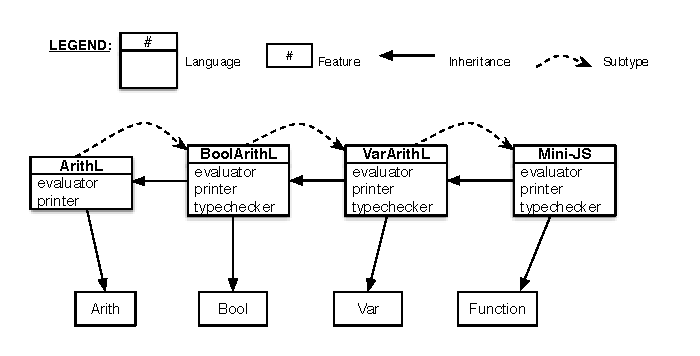
\includegraphics{dependency.eps}
%   \caption{Overview of the language components.}
%   \label{fig:dependency}
% \end{figure}

\subsection{Evaluation}
\label{sec:evaluate}

To evaluate \name's implementation of the case study,
\Cref{fig:sloc} compares the number of source lines of code
(SLOC, lines of code without counting empty lines and comments) for
\name's \emph{modular} implementation with the vanilla
\emph{non-modular} AST-based implementations in Haskell. The Haskell
implementations are just straightforward AST interpreters, which duplicate code across the multiple language
components.

Since \name is a new language, we
had to write various code that is provided in Haskell by the standard library,
so they are not counted for fairness of comparison. In the left part, for each
feature, we count the lines of the algebra interface (number beside the feature
name), and the algebras for the operations. In the right part, for each
language, we count the lines of ASTs, and those to combine previously
defined operations. For example, here is the code that is needed to make the
\lstinline{arith} language.
\lstinputlisting[linerange=537-544]{../../examples/case_study.sl}% APPLY:linerange=ARITH
We only need 8 lines in total: 2 lines for the AST, and 6 lines to combine the operations.

Therefore, the total SLOC of \name's implementation is the sum of all the
lines in the feature and language parts (237 SLOC of all features plus 94 SLOC
of ASTs and operations). Although \name is considerably more verbose than a
functional language like Haskell, \name's modular implementation for 12 languages and 30
operations in total reduces approximately 60\% in terms of SLOC. The reason is
that, the more frequently a feature is reused by other languages directly or
indirectly, the more reduction we see in the total SLOC. For example,
$\mathit{natF}$ is used across many languages. Even though \lstinline{simplenat}
itself \emph{alone} has more SLOC ($40 = 7+23+7+3$) than that of Haskell (which
has 33), we still get a huge gain when implementing other languages.

Finally, we acknowledge the limitation of our case study in that SLOC is just
one metric and we have not measured any other metrics. Nevertheless we believe
that the case study is already non-trivial in that we need to solve EP. Note
that Scala traits alone are not sufficient on their own to solve EP. While there
are solutions to EP in both Haskell and Scala, they
introduce significant complexity, as explained in \cref{sec:ob}.



\begin{figure}[t]
  \centering
  \begin{small}
  \begin{tabular}{|r|ccc||l|ccc|}
    \hline
     Feature & \textbf{eval} & \textbf{print} & \textbf{check} & Lang name & \name & \textbf{Haskell} & \textbf{\% Reduced}  \\
    \hline
    $\mathit{natF}$(7) & 23 & 7 & 39 & \lstinline$simplenat$ & 3 & 33 & 91\%  \\
    $\mathit{boolF}$(4) & 9 & 4 & 17 & \lstinline$simplebool$ & 3 & 16 & 81\% \\
    $\mathit{compF}$(4) & 12 & 4 & 20 & \lstinline$natbool$ & 5 & 74 & 93\% \\
    $\mathit{logicF}$(4) & 12 & 4 & 20 & \lstinline$varbool$ & 4 & 24 & 83\% \\
    $\mathit{varF}$(4) & 7 & 4 & 7 & \lstinline$varnat$ & 4 & 41 & 90\% \\
    $\mathit{funcF}$(3) & 10 & 3 & 9 & \lstinline$simplelogic$ & 4 & 28 & 86\% \\
     & & & & \lstinline$varlogic$ & 6 & 36 & 83\% \\
     & & & & \lstinline$arith$ & 8 & 94 & 91\% \\
     & & & & \lstinline$arithlogic$ & 8 & 114 & 93\% \\
     & & & & \lstinline$vararith$ & 8 & 107 & 93\% \\
     & & & & \lstinline$vararithlogic$ & 8 & 127 & 94\% \\
     & & & & \lstinline$mini-JS$ & 33 & 149 & 78\% \\
    \hline
    \bf{Total} & & & 237 & & 331 & 843 & 61\% \\
    \hline
  \end{tabular}
  \end{small}
  \caption{SLOC statistics: \name implementation vs vanilla AST implementation.}
  \label{fig:sloc}
\end{figure}




\begin{comment}
\subsection{Putting all together}

% With all the components ready, we can assemble them at will to cook a language
% with whatever features we want. For example, we hope by now the reader can share
% our feeling that this is indeed a simple and modular way to cook a language
% incrementally.

To demonstrate the usage of the final language \lstinline{MiniJS}, here is a function that
makes sure ``well-typed programs cannot go wrong'':
\lstinputlisting[linerange=-]{}% APPLY:linerange=SUPER_DEF
It type checks the program before passing it to the evaluator and pretty
printer.

% we first create a program that
% uses all the features the language supports now.
% \lstinputlisting[linerange=-]{}% APPLY:linerange=FINAL_TEST
% The concrete syntax of the program is shown in the comment above. We assume a
% pre-defined function environment (\lstinline{fenv}) containing the definition of
% the \lstinline{add1} function.

% Finally we apply it to the program we have just created:
% \lstinputlisting[linerange=735-736]{../../examples/case_study.sl}% APPLY:linerange=TEST_TEST
% Everything works as expected!
\end{comment}

\begin{comment}
\subsection{Parameterizing Expressions by the Evaluation Order}

We now turn to the second case study. In this case study, we embed a
higher-order domain-specific language inside \name. Our object language in this
case study is typed lambda calculus with conditional and constants. This time,
the embedding not only demonstrates the extensibility, as is shown in the first
case study, but also object types, expressed in the meta-language (\name) and
manifestly ensuring well-scoped and well-typed expressions in the object
language. What is more, the evaluator over the object expressions is type
preserving by construction. The embedding of typed languages is directly
inspired by Kiselyov's lecture notes~\cite{kiselyov2012typed} on the
"tagless-final" approach to embedding languages.

\paragraph{Well-typed object expressions} One important issue with such
embedding is how to deal with binders in the object language. In general there
are two options, one can either use deBrujin indices~\cite{}, or higher-order
abstract syntax (HOAS)~\cite{}. Each option has its cons and pros, but for this
particular case study, we find HOAS convenient. HOAS represents object language
abstractions as \name abstractions and object variables as \name variables. By
utilizing the infrastructure of the meta-language, we are free of issues such as
variable capture. Here is the interface of the object language.
\lstinputlisting[linerange=-]{}% APPLY:linerange=TYPED_LAMBDA
Embedded object expressions of type \lstinline{A} are represented as \name
values of the type \lstinline{Expr[A]}. The \lstinline{bot} constructor, which
represents non-terminating computation, is there for the purpose of illustrating
different evaluation strategies.

A careful reader may notice that the \lstinline{ExprAlg} interface has no
abstractions. This is intentional! Evaluators with different evaluation
strategies only differ in the interpretation for abstractions, as will be shown
later on. For this reason, \lstinline{lam} is moved to a separate interface of
its own.
\lstinputlisting[linerange=-]{}% APPLY:linerange=ABSTRACTION


\paragraph{Well-typed evaluator}
The benefit of typeful embedding shows up when defining the evaluator.
\lstinputlisting[linerange=-]{}% APPLY:linerange=TYPED_EVAL
Unlike the evaluator in the first case study, there is no need for a separate
\lstinline{Value} datatype for values, as they are directly modeled by \name
values. Note that the resulting evaluator is \emph{type preserving} by
construction.

\paragraph{Call-by-name, call-by-value}
Our evaluator defined in the first case study inherits the evaluation strategy
from the meta-language. We now show call-by-name and call-by-value evaluators.
The two evaluators are quite alike, sharing most of the code. As said before,
the only difference is the interpretation for \lstinline{lam}.
\lstinputlisting[linerange=-]{}% APPLY:linerange=CBN_CBV
The call-by-name \lstinline{lam}, when applied, will receive an unevaluated
argument expression, use it as it is. The call-by-value \lstinline{lam}, as in
the call-by-name evaluator, receives an unevaluated argument expression,
evaluates it before passing its result to the abstraction body \lstinline{f}.

Now to make an evaluator parameterized over the evaluation order, we just take a
trait \lstinline{o} with unknown implementation, compose it with other language
features.
\lstinputlisting[linerange=-]{}% APPLY:linerange=MAKE_EVAL
Here is the call-by-name evaluator at work:
\lstinputlisting[linerange=-]{}% APPLY:linerange=CBN_TEST
On the other hand, \lstinline{(evaluator evalBindCBV ex)()} would result in a
infinite loop. The complete code with several examples can be found in the
supplementary materials.

\jeremy{I am afraid we don't seem to have many advantages over OCaml's version,
  because we don't really have higher-kinded types, we cannot make a AST type
  for this example, though \lstinline{makeEvaluator} seems to be one advantage }

\end{comment}

%%% Local Variables:
%%% mode: latex
%%% TeX-master: "../paper"
%%% org-ref-default-bibliography: ../paper.bib
%%% End:


% \section{Desugaring}
\label{sec:desugar}

\name is built upon a thin-layer of sugar on top of
\bname~\cite{alpuimdisjoint}. \bname is a polymorphic language with subtyping,
and it was developed as an alternative to languages such as System $F_{<:}$ to
serve as a core language for OO languages. The choice of \bname is due to its
support for disjoint intersection types and disjoint polymorphism (used to model
subtyping and conflict detection), and the so-called merge construct (which is
used to model dynamic trait inheritance). The theoretical aspects of \bname
(including the formalization of the static and dynamic semantics, and the proofs
of type safety and coherence) were already studied in previous work. So they are
not a contribution of this paper and are not necessary to understand the
desugaring process.

The novelty in this section is to explain how to build a high-level OO
abstractions on top of the core constructs of \bname. In particular we focus on
how the trait system presented in this paper is built. The key idea behind trait
translation is inspired by the functional mixin semantics using open recursion,
which is proposed by~\citet{cook1989denotational} in an untyped setting.
However, our translation is done in the context of a statically-typed
programming language, which is exactly why conflicts can be \textit{statically}
detected in traits.

\subsection{A Brief Introduction to \bname}
The syntax of our core language \bname is shown in Figure~\ref{fig:synax-fi}.

\paragraph{Types}
Apart from normal type constructs, the main novelty are two constructs used to
support disjoint intersection types and disjoint polymorphism: intersection
types $[[A & B]]$ and disjoint (universal) quantification $[[ forall ( a ** A )
. B ]]$. \bname also includes singleton record types $[[{ l : A}]]$ and type
applications $[[ T [ B1 , .. , Bn ] ]]$.

\paragraph{Terms}
In correspondence with types, terms include merges $[[E1 ,, E2]]$, abstraction
of type variables over terms $[[blam ( a ** A ) . E]]$, applications of terms to
types $[[E A]]$, and singleton records $[[ { l = E } ]]$. Record operations are
projections $[[E.l]]$ and exclusions $[[E -- { l : A }]]$. We also have
recursive \lstinline{let} bindings.

\paragraph{Type and term declarations}

For the convenience of writing large programs, we also support type and term
declarations. A type declaration declares a type constructor's name $T$, its
type parameters and its definition $A$. A term declaration declares a function's
name $f$, its parameter signatures, its result type $B$, and its function body
$e$. Although previous work does not have declarations, we do not think adding
them will cause any problems to the meta-theory of \bname. A careful study of
these additions is of course a good avenue for future work.

\paragraph{Syntactic sugar} Multi-field record types are encoded as
intersections of singleton record types, and multi-field records as merges of
singleton records.

% \bruno{I think we can omit most of the primitive types and operations
%   from the formal syntax. You should present the syntactic sugar for
%   (multi-field) records and record types in the figure.}
% \bruno{Briefly explain the key novel contructs: merge, big lambda }
% \bruno{Explain that declarations/programs are new, but we don't think
%   this will cause any programs to the meta-theory.}

\begin{figure}[t]
\centering
\begin{small}
\begin{tabular}{lrcl}
  Types  & $[[A]], [[B]]$ & ::= & $[[top]] \mid [[Int]] \mid [[A -> B]] \mid [[A & B]] \mid  [[{ l : A }]] \mid [[a]] \mid [[forall ( a ** A ) . B]] \mid [[ T [ B1 , .. , Bn ] ]]$ \\
  Expressions & $[[E]]$ & ::= & $[[()]] \mid [[N]] \mid [[x]] \mid [[\ x . E]] \mid [[E1 E2]] \mid [[blam ( a ** A ) . E]] \mid [[E A]] \mid [[E1 ,, E2]] $ \\
         & & $\mid$ & $[[let x : A = E1 in E2]] \mid [[{ l = E }]] \mid [[E . l]] \mid [[E -- { l : A }]] $ \\
  Programs & $[[pgm]]$ & ::= & $[[decl1 .. decln E]]$ \\
  Declarations & $[[decl]]$ & ::= & $[[ def f ( x1 : A1 ) .. ( xn : An ) : B = E ]] \mid [[ type T [ a1 , .. , an ] = A ]]$ \\ \\
\end{tabular}
\begin{tabular}{llll}
  Record types & $[[ { l1 : A1 , ... , ln : An } ]] $ & := & $[[ { l1 : A1} & ... & { ln : An } ]]$ \\
  Records &  $[[ { l1 = E1 , ... , ln = En } ]] $ & := & $ [[ { l1 = E1 } ,, ... ,, { ln = En } ]]$
\end{tabular}
\end{small}
\caption{\bname syntax and syntactic abbreviations}
\label{fig:synax-fi}
\end{figure}

\subsection{Desugaring Traits}

\paragraph{Trait declarations}

The left part of Figure~\ref{fig:trans-trait} presents the translation of trait
declarations. Essentially traits are translated into term declarations, with
methods becoming record fields. The self-reference is adjusted to be the last
parameter of the declaration. For example
\lstinputlisting[linerange=13-13]{../examples/point.sl}% APPLY:linerange=DESUGAR1
becomes
\begin{lstlisting}
def point3D (x : Double) (y : Double) (self : Point3D) = point x y self ,, { z = self.x }
\end{lstlisting}
Now it is clear that \lstinline{self} is not a special keyword: it can have any
name.

% To account for the call-by-value semantics of the
% target language, the type of the self-reference $s$ has become a thunk
% \lstinline[mathescape=true]{T -> $A_0$}, and the occurrences of the
% self-reference \lstinline{s} in the trait body are replaced by \lstinline{s()}.


\paragraph{Instantiation of traits}

The right part of Figure~\ref{fig:trans-trait} shows the translation of trait
instantiation. Specifically, the self-reference gets passed to each trait $m_1$
to $m_n$, as each of them is an open term after translation. The results are
then merged to form a new term. \lstinline{new} instantiates a trait by
taking the \textit{lazy fixpoints} of the resulting term. For example,
\lstinline{new[Point3D] point3D(3,4)} is translated into \lstinline{let self : Point3D = point3D 3 4 self in self}.
% \name has a lazy (and possibly recursive) \lstinline{let} construct.


% Lazy fixpoints are implemented in \name using the built-in \lstinline{let}
% construct (possibly recursive), which employs call-by-name semantics. It is
% possible to choose call-by-value, then the type of the self-reference would
% become a thunk (e.g., \lstinline$T -> Point$) to prevent premature evaluation.


\paragraph{The type for traits}

\lstinline[mathescape=true]{Trait[$T_1, T_2$]} denotes the type of those traits
which provide an interface described by the type $T_2$ with dependency on $T_1$.
In fact, it is simply translated into $T_1 \rightarrow T_2$.

\begin{figure}[t]
  \centering
  \begin{tabular}{l|l}

\begin{lstlisting}[mathescape=true]
trait m ($x_1 : A_1$, ..., $x_n : A_n$)
  inherits $a_1$ & ... & $a_m$ { $s : A_0$ =>
  def $m_1$(..) = $e_1$
  ..
  def $m_s$(..) = $e_s$ }
\end{lstlisting} &

\begin{lstlisting}[mathescape=true]
new[A] $m_1$ & ... & $m_n$
\end{lstlisting}  \\

    $\rightsquigarrow$  & $\rightsquigarrow$ \\

\begin{lstlisting}[mathescape=true]
def m $(x_1 : A_1)$ ... $(x_n : A_n)$ $(s : A_0)$
  = $a_1$(s) ,, ... ,, $a_m$(s) ,,
{ $m_1$ = \(..) -> $e_1$
, ..
, $m_s$ = \(..) -> $e_s$ }
\end{lstlisting} &


\begin{lstlisting}[mathescape=true]
let self : A =
  $m_1$(self) ,, ... ,, $m_n$(self)
in self
\end{lstlisting}
  \end{tabular}
  \caption{Translations of trait declaration (left) and trait instantiation (right).}
\label{fig:trans-trait}

\end{figure}



\section{Implementation and Discussion}

\name implementation is done in Haskell, and is structured around a typed core language
(\bname with some extensions). The overall implementation is unremarkable, as it
closely follows the semantics presented by~\citet{alpuimdisjoint}. It consists
of 3 phases: 1) The desugaring phase (cf. Section~\ref{sec:desugar}) takes an
abstract syntax tree (AST) generated by the parser, and returns a \bname
expression. Trait-related constructs disappear after this phase; 2) the type
checking phase then takes a \bname expression from the previous phase, it infers
and checks its type, and in the meantime, produces an expression in the target
language; and 3) the target expression (call-by-name pure untyped lambda
calculus) then enters the final phase, and is executed by a simple interpreter.

% The main component of the implementation is an
% elaborating type-checker, which takes a \bname expression, checks it, and
% produces another expression in the target language. The final expression is then
% directly executed by an interpreter. We chose call-by-value untyped lambda
% calculus as the target language. Since we focus on the implementation, and types
% are irrelevant after type checking, the untyped lambda calculus is a suitable choice
% with minimal syntax.


The type checker is the most involved component in the pipeline. It contains a
(coercive) subtyping procedure and a disjointness checker, both of which are the
most critical parts in \name. In regard to the subtyping rules, in addition to what have
been presented~\citep{alpuimdisjoint}, we have an additional rule, which we
found helpful for enabling the composition of Object Algebras. For brevity, we
only show a simplified version below: \ottusedrule{\ottdruleSubXXR{}} By this
rule, one can derive for example,
$$
[[ { l : Int -> String} & { l : Bool -> Bool}]] <: [[ { l : Int & Bool -> String & Bool}]]
$$
We believe this rule would not endanger the type
system, as it is orthogonal to the other subtyping rules. Besides, our
preliminary meta-theory study shows that the new subtype system enjoys the same
properties as before.

% The prototype implementation is written in just 1400 lines of Haskell code.

% \begin{figure}[t]
%   \centering
%   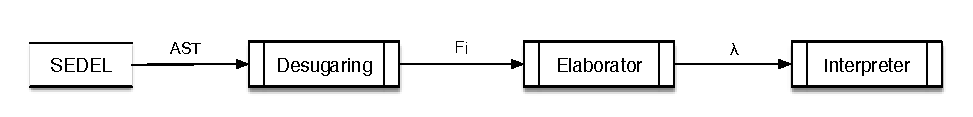
\includegraphics[scale=0.9]{pipeline.eps}
%   \caption{The pipeline of \name}
%   \label{fig:pipeline}
% \end{figure}

% 
\section{Discussion}
\label{sec:discussion}

In this section we consider a simple extension to the language to further
demonstrate the applicability of our definition of consistent subtyping. We also
discuss the design decisions involved in the algorithmic system and show how it
helps address the issue arising from the ambiguity of the type-directed
translation.

\subsection{Extension with Top}
\label{subsec:extension-top}

We argued that our definition of consistent subtyping (\Cref{def:decl-conssub})
is a \textit{general} definition in that it is independent of language features.
We have shown its applicability to polymorphic types, for which neither
\citet{siek2007gradual} nor the AGT approach~\citep{garcia2016abstracting} can
be extended naturally. To strengthen our argument, we consider extending the
language with the $\tope$ type and show that our approach naturally embraces the
extension, with all the desired properties preserved. To aid comparison, we also
show how to adapt the AGT approach to support $\tope$ and verify that these two
approaches, though rooted in different foundations, coincide again on
\textit{simple types}. However, \Cref{def:old-decl-conssub} of
\citet{siek2007gradual} fails to support $\tope$.


\paragraph{Extending Definitions}

In order to preserve the orthogonality between subtyping and consistency, we
require $\top$ to be a common supertype of all static types, as shown in rule
\rul{S-Top}. This rule might seem strange at first glance, since even
if we remove
the requirement $A~static$, the rule seems reasonable.
However, the important point is that because of the orthogonality between
subtyping and consistency, subtyping itself should not contain a potential cast
in principle! Therefore, subtyping instances such as $\unknown \tsub \top$ are not allowed.
For consistency, we add the rule that $\top$ is consistent with $\top$, which is
actually included in the original reflexive rule $A \sim A$. For consistent
subtyping, every type is a consistent subtype of $\top$, for example, $\nat \to
\unknown \tconssub \top$.
\begin{mathpar}
  \SubTop \and \CTop \and \CSTop
\end{mathpar}
It is easy to verify that \Cref{def:decl-conssub} is still equivalent to that in
\Cref{fig:decl:conssub} extended with rule \rul{CS-Top}. That is,
\Cref{lemma:properties-conssub} holds:
\begin{mprop}[Extension with $\top$]
  The following are equivalent:
  \begin{itemize}
  \item  $\tpreconssub A \tconssub B$.
  \item  $\tpresub A \tsub C$, $C \sim D$, $\tpresub D \tsub B$, for some $C, D$.
  \end{itemize}
\end{mprop}
% \begin{proof}\leavevmode
%   \begin{itemize}
%   \item From first to second: By induction on the derivation of consistent
%     subtyping. We have extra case \rul{CS-Top} now, where $B = \top$.
%     We can choose $C = A$, and
%     $D$ by replacing the unknown types in $C$ by $\nat$. Namely, $D$ is a static
%     type, so by \rul{S-Top} we are done.
%   \item From second to first: By induction on the derivation of second
%     subtyping. We have extra case \rul{S-Top} now, where
%     $B = \top$, so $A \tconssub B$ holds by \rul{CS-Top}.
%   \end{itemize}
% \end{proof}

\paragraph{Extending AGT}

We now extend the definition of concretization (\Cref{def:concret}) with $\top$
by adding another equation:
\[
  \gamma(\top) = \{\top\}
\]
It is easy to verify that \Cref{lemma:coincide-agt} still holds:
\begin{mprop}[Equivalent to AGT Extended with $\top$ on Simple Types]
  \label{prop:agt-top}
  $A \tconssub B$ if only if $A \agtconssub B$.
\end{mprop}

% \begin{proof}\leavevmode
%   \begin{itemize}
%   \item From left to right: By induction on the derivation of consistent
%     subtyping. We have case \rul{CS-Top} now.
%     It follows that for
%     every static type $A_1 \in \gamma(A)$, we can derive $A_1 \tsub \top$ by
%     \rul{S-Top}.
%     We have $B_1 = B = \top$ and we are done.
%   \item From right to left: By induction on the derivation of subtyping and
%     inversion on the concretization. We have extra case \rul{S-Top} now, where
%     $B$ is $\top$. So
%     consistent subtyping directly holds.
%   \end{itemize}
% \end{proof}

\paragraph{\citeauthor{siek2007gradual}'s definition of consistent subtyping does not work for $\top$}

Similarly to the analysis in \Cref{subsec:towards-conssub}, $\nat \to \unknown
\tconssub \top$ only holds when we first apply consistency, then subtyping, as
shown in the following diagram. However we cannot find a type $A$ such that
$\nat \to \unknown \tsub A$ and $A \sim \top$. Also we have a similar problem in
extending the restriction operator: \textit{non-structural} masking between
$\nat \to \unknown$ and $\top$ cannot be easily achieved.
\begin{center}
  \begin{tikzpicture}
    \matrix (m) [matrix of math nodes,row sep=3em,column sep=4em,minimum width=2em]
    {
      \bot & \top \\
      \nat \to \unknown &
      \nat \to \nat \\};

    \path[-stealth]
    (m-2-1) edge node [left] {$\tsub$} (m-1-1)
    (m-2-2) edge node [left] {$\tsub$} (m-1-2);

    \draw
    (m-1-1) edge node [above] {$\sim$} (m-1-2)
    (m-2-1) edge node [below] {$\sim$} (m-2-2);
  \end{tikzpicture}
\end{center}


\subsection{Better to be Unknown}
\label{subsec:algo:discuss}

In \Cref{sec:type:trans} we have seen an example where a source expression could
produce two different target expressions with different runtime behaviour. As we
explained, this is due to the guessing nature of the declarative system, and
from the typing point of view, no type is particularly better than others.
However in practice, this is not desirable. Let us revisit the same example, now
from the algorithmic point of view (we omit the translation for space reasons,
the interested reader can try to write down the full derivation):
\[
  f: \forall a. a \to a \byinf (\blam x \unknown {f ~ x}) \infto \unknown \to \genA \dashv f : \forall a. a \to a, \genA
\]
Compared with declarative typing, which can produce as many types as
possible ($\unknown \to \nat$, $\unknown \to \bool$, and so on), the algorithm
computes the type $\unknown \to \genA$ with $\genA$ unsolved in the output
context. This is due to rule \rul{ACS-UnknownL}. What can we know from the
output context? The only thing we know is that $\genA$ is not constrained at
all! As we discussed, any monotype for $\genA$ is inappropriate. Instead, we
replace $\genA$ with the unknown type $\unknown$, which helps to avoid unnecessary
down-casts at runtime (any cast to $\unknown$ is safe), resulting in the final
type $\unknown \to \unknown$.


\paragraph{Do soundness and completeness still hold?}

The reader may ask if the declarative system produces types such as $\unknown
\to \nat$ and $\unknown \to \bool$, but the algorithmic system computes the type
$\unknown \to \unknown$, does it imply that the algorithmic system is no longer
sound and complete with respect to the declarative system? The answer is no.
First of all, note that \Cref{thm:type_complete} reads ``$\dots$ there exist
$\Delta$, $\Omega'$ and $A'$ such that $\dots$ $A = \ctxsubst{\Omega'}{A'}$''.
Now if $A'$ (which is produced by the algorithmic system) contains some unsolved
existential variables, it is up to us to pick solutions in $\Omega'$ to match up
with $A$ (which is produced by the declarative system). More concretely, let us
assume that the declarative system produces type $\unknown \to \nat$, and let
$\Omega = f : \forall a. a \to a$ and $\Delta = f : \forall a. a \to a, \genA$,
the completeness theorem asks if we can find a complete context $\Omega'$ that
extends both $\Delta$ and $\Omega$ such that $\ctxsubst{\Omega'}{(\unknown \to
  \genA)} = \unknown \to \nat$. It is obvious that $\Omega' = f : \forall a. a
\to a, \genA = \nat$ is one such complete context, and we have
$\ctxsubst{\Omega'}{(\unknown \to \genA)} = \unknown \to \nat$. So the
algorithmic system is still complete. Similar arguments apply to the soundness
theorem. 
Secondly, an observation (which follows from the soundness and
completeness theorems) is: if an
expression is typeable with many types in the declarative system, the same expression must be
typeable with a single type that contains some unsolved existential variables in the algorithmic
algorithmic system.
In that case, replacing them with $\unknown$ is the best
strategy for the sake of execution.

\paragraph{Existential variables do not indicate parametricity}

Another reading of the above example may suggest that the result type $\unknown
\to \genA$ implies parametricity, with the implication that $\genA$ can be
changed arbitrarily without affecting the runtime behaviour of the
program. A similar phenomenon is discussed by \citet{siek2008gradual}, where they
argue that we cannot simply ``ignore dynamic types during unification''. In
their view, a type signature with a type variable indicates parametricity, but
this type does not. We agree that type variables do indicate parametricity, but
\textit{existential variables} do not! An \textit{unsolved} existential variable
indicates that a value's only constraint is that it may be cast to and from
$\unknown$, thus may introduce runtime casts. A similar observation is also
found in \citet{garcia2015principal}, where they have to distinguish between
\textit{static polymorphism} and \textit{gradual polymorphism}, and in addition
to gradual type parameters, they have to introduce the so-called \textit{static
  type parameters}. We argue that our language design is much simpler, and our
algorithmic system naturally embraces this distinction.

Now the question is can we really do that? The syntax in \Cref{fig:algo-syntax}
specifies that the solution of a existential variable can only be a monotype.
This is true if the existential variable has a solution. Reading of the output
context reveals that $\genA$ does not have any solution at all. What is more,
our target language (i.e., \pbc) has a nice property, the so-called
``Jack-of-All-Trade Principle''~\cite{ahmed2011blame} that says if instantiating
a type parameter to any given type yields an answer then instantiating that type
parameter to $\unknown$ yields the same answer. In light of these, no type is
more suitable than $\unknown$.

We need to note that this does not mean we should always instantiate a type
parameter to $\unknown$, as is the case in \pbc. One of our design principles is
that we should extract as much information as possible from the static aspects of
the type system, until there is nothing more we can know, then leave the job to
the runtime checks.



%%% Local Variables:
%%% mode: latex
%%% TeX-master: "../paper"
%%% org-ref-default-bibliography: "../paper.bib"
%%% End:



\section{Related Work}
\label{sec:related}

Along the way we discussed some of the most relevant work to motivate,
compare and
promote our gradual typing design. In what follows, we briefly discuss related
work on gradual typing and polymorphism.


\paragraph{Gradual Typing}

The seminal paper by \citet{siek2006gradual} is the first to propose gradual
typing, which enables programmers to mix static and dynamic typing in a program
by providing a mechanism to control which parts of a program are statically
checked. The original proposal extends the simply typed lambda calculus by
introducing the unknown type $\unknown$ and replacing type equality with type
consistency. Casts are introduced to mediate between statically and dynamically
typed code. Later \citet{siek2007gradual} incorporated gradual typing into a
simple object oriented language, and showed that subtyping and consistency are
orthogonal -- an insight that partly inspired our work. We show that subtyping
and consistency are orthogonal in a much richer type system with higher-rank
polymorphism. \citet{siek2009exploring} explores the design space of different
dynamic semantics for simply typed lambda calculus with casts and unknown types.
In the light of the ever-growing popularity of gradual typing, and its somewhat
murky theoretical foundations, \citet{siek2015refined} felt the urge to have a
complete formal characterization of what it means to be gradually typed. They
proposed a set of criteria that provides important guidelines for designers of
gradually typed languages. \citet{cimini2016gradualizer} introduced the
\emph{Gradualizer}, a general methodology for generating gradual type systems
from static type systems. Later they also develop an algorithm to generate
dynamic semantics~\cite{CiminiPOPL}. \citet{garcia2016abstracting} introduced
the AGT approach based on abstract interpretation. As we discussed, none of
these approaches instructed us how to define consistent subtyping for
polymorphic types.

There is some work on integrating gradual typing with rich type disciplines.
\citet{Ba_ados_Schwerter_2014} establish a framework to combine gradual typing and
effects, with which a static effect system can be transformed to a dynamic
effect system or any intermediate blend. \citet{Jafery:2017:SUR:3093333.3009865}
present a type system with \emph{gradual sums}, which combines refinement and
imprecision. We have discussed the interesting definition of \emph{directed
  consistency} in Section~\ref{sec:exploration}. \citet{castagna2017gradual} develop a gradual type system with
intersection and union types, with consistent subtyping defined by following
the idea of \citet{garcia2016abstracting}.
TypeScript~\citep{typescript} has a distinguished dynamic type, written {\color{blue} any}, whose fundamental feature is that any type can be
implicitly converted to and from {\color{blue} any}.
% They prove that the conversion
% definition (called \emph{assignment compatibility}) coincides with the
% restriction operator from \citet{siek2007gradual}.
Our treatment of the unknown type in \cref{fig:decl:conssub} is similar to their
treatment of {\color{blue} any}. However, their type system does not have
polymorphic types. Also, Unlike our consistent subtyping which inserts runtime
casts, in TypeScript, type information is erased after compilation so there are
no runtime casts, which makes runtime type errors possible.
% dynamic checks does not contribute to type safety.


\paragraph{Gradual Type Systems with Explicit Polymorphism}

\citet{Morris:1973:TS:512927.512938} dynamically enforces
parametric polymorphism and uses \emph{sealing} functions as the
dynamic type mechanism. More recent works on integrating gradual typing with
parametric polymorphism include the dynamic type of \citet{abadi1995dynamic} and
the \emph{Sage} language of \citet{gronski2006sage}. None of these has carefully
studied the interaction between statically and dynamically typed code.
\citet{ahmed2011blame} proposed \pbc that extends the blame
calculus~\cite{Wadler_2009} to incorporate polymorphism. The key novelty of
their work is to use dynamic sealing to enforce parametricity. As such, they end
up with a sophisticated dynamic semantics. Later, \citet{amal2017blame} prove
that with more restrictions, \pbc satisfies parametricity. Compared to their
work, our type system can catch more errors earlier since, as we argued, 
their notion of \emph{compatibility} is too permissive. For example, the
following is rejected (more precisely, the corresponding source program never
gets elaborated) by our type system:
\[
  (\blam x \unknown x + 1) : \forall a. a \to a \rightsquigarrow \cast {\unknown \to \nat}
  {\forall a. a \to a} (\blam x \unknown x + 1)
\]
while the type system of \pbc would accept the translation, though at runtime,
the program would result in a cast error as it violates parametricity.
% This does not imply, in any regard that \pbc is not well-designed; there are
% circumstances where runtime checks are \emph{needed} to ensure
% parametricity.
We emphasize that it is the combination of our powerful type system together
with the powerful dynamic semantics of \pbc that makes it possible to have
implicit higher-rank polymorphism in a gradually typed setting.
% without compromising parametricity.
\citet{devriese2017parametricity} proved that
embedding of System F terms into \pbc is not fully abstract. \citet{yuu2017poly}
also studied integrating gradual typing with parametric polymorphism. They
proposed System F$_G$, a gradually typed extension of System F, and System
F$_C$, a new polymorphic blame calculus. As has been discussed extensively,
their definition of type consistency does not apply to our setting (implicit
polymorphism). All of these approaches mix consistency with subtyping to some
extent, which we argue should be orthogonal. On a side note, it seems that our
calculus can also be safely translated to System F$_C$. However we do not
understand all the tradeoffs involved in the choice between \pbc and System
F$_C$ as a target.



\paragraph{Gradual Type Inference}
\citet{siek2008gradual} studied unification-based type inference for gradual
typing, where they show why three straightforward approaches fail to meet their
design goals. One of their main observations is
that simply ignoring dynamic types during unification does not work. Therefore,
their type system assigns unknown types to type variables and infers gradual
types, which results in a complicated type system and inference algorithm. In
our algorithm presented in \cref{sec:advanced-extension}, comparisons between
existential variables and unknown types are emphasized by the distinction
between static existential variables and gradual existential variables. By
syntactically refining unsolved gradual existential variables with unknown types, we gain a
similar effect as assigning unknown types, while keeping the algorithm relatively
simple.
\citet{garcia2015principal} presented a new approach where gradual type
inference only produces static types, which is adopted in our type system. They
also deal with let-polymorphism (rank 1 types). They proposed the distinction
between static and gradual type parameters, which inspired our extension to
restore the dynamic gradual guarantee. Although those existing works all involve
gradual types and inference, none of these works deal with higher-rank
implicit polymorphism.


\paragraph{Higher-rank Implicit Polymorphism}

\citet{odersky1996putting} introduced a type system for higher-rank implicit
polymorphic types. Based on that, \citet{jones2007practical} developed an
approach for type checking higher-rank predicative polymorphism.
\citet{dunfield2013complete} proposed a bidirectional account of higher-rank
polymorphism, and an algorithm for implementing the declarative system, which
serves as the main inspiration for our algorithmic system. The key difference,
however, is the integration of gradual typing.
% \citet{vytiniotis2012defer}
% defers static type errors to runtime, which is fundamentally different from
% gradual typing, where programmers can control over static or runtime checks by
% precision of the annotations.
As our work, those works are in a
\emph{predicative} setting, since complete type inference for higher-rank
types in an impredicative setting is undecidable. Still, there are many type
systems trying to infer some impredicative types, such as
\texttt{$ML^F$}~\citep{le2014mlf,remy2008graphic,le2009recasting}, the HML
system~\citep{leijen2009flexible}, the FPH system~\citep{vytiniotis2008fph} and
so on. Those type systems usually end up with non-standard System F types, and
sophisticated forms of type inference.

%%% Local Variables:
%%% mode: latex
%%% TeX-master: "../paper"
%%% org-ref-default-bibliography: "../paper.bib"
%%% End:



\section{Conclusion and Future Work}
\label{sec:conclusion}

We have proposed \fnamee, a type-safe and coherent calculus with disjoint
intersection types, BCD subtyping and parametric polymorphism. \fnamee improves
the state-of-art of compositional designs, and enables the development of highly
modular and reusable programs. One interesting and useful further extension
would be implicit polymorphism. For that we want to combine
Dunfield and Krishnaswami's approach~\cite{dunfield2013complete} with our bidirectional type system.
We would also like to study the parametricity of \fnamee. As we have seen in
\cref{sec:failed:lr}, it is not at all obvious how to extend the standard
logical relation of System F to account for disjointness, and avoid potential
circularity due to impredicativity. A promising solution is to use step-indexed
logical relations~\cite{ahmed2006step}. 
% TOM: This sentence is broken. Do we even need it?
% We have yet investigated further on that direction.


\section*{Acknowledgments}

We thank the anonymous reviewers and Yaoda Zhou for their helpful comments.
This work has been sponsored by the Hong Kong Research Grant
Council projects number 17210617 and 17258816, and by the Research Foundation -
Flanders.



%%% Local Variables:
%%% mode: latex
%%% TeX-master: "../paper"
%%% org-ref-default-bibliography: "../paper.bib"
%%% End:


%%
%% Bibliography
%%

%% Please use bibtex,

\bibliography{paper}


% \newpage
% \appendix
% \section{Specification and Metatheory of \ecore}
We give the specification and metatheory of \ecore in this section. We
have completely formalized proofs of metatheory in Coq based on
Chargu{\'e}raud's work~\citeapp{charcoq}. We also provide brief paper
proofs for \ecore for reference. Full proofs can be found in the Coq
scripts\footnote{\fullurl} \verb|WeakCast_*.v|. The corresponding name of
each lemma in Coq is marked at the beginning in brackets.

\subsection{Syntax}
\begin{center}
\begin{minipage}{0.55\textwidth}
\gram{\ottec}
\end{minipage}
\begin{minipage}{0.4\textwidth}
\gram{
  \ottGg\ottinterrule
  \ottv}
\end{minipage}
\\
\end{center}
\begin{tabular}{ll}
Syntactic Sugar \\
& $\ottcoresugar$ % defined in otthelper.mng.tex
\end{tabular}

\subsection{Operational Semantics}
\ottdefnstep{}
% \ottusedrule{\ottdruleSXXMu{}}

\subsection{Typing}
\ottdefnctx{}\ottinterrule
\ottdefnexpr{}
% \ottusedrule{\ottdruleTXXMu{}}

\subsection{Properties}
\begin{comment}
We follow the naming of lemmas and proofs of properties 
for Pure Type System from \citeapp{handbook}. Some lemmas have other well-known names, like
Lemma \ref{lem:appendix:thin} is often called \emph{Weakening} and 
Lemma \ref{lem:appendix:gen} is often called \emph{Inversion}.

\begin{lemma}[Free Variable]\label{lem:appendix:free}
    If $[[G |- e:t]]$, then $\FV(e) \subseteq \dom([[G]])$ and $\FV([[t]])
\subseteq \dom([[G]])$.
\end{lemma}

\begin{proof}
    By induction on the derivation of $[[G |- e:t]]$. We only treat cases
\ruleref{T\_Mu}, \ruleref{T\_CastUp} and \ruleref{T\_CastDown} (since proofs of
other cases are the same as \cc \citeapp{handbook}):
    \begin{description}
        \item[Case \ruleref{T\_Mu}:] From premises of $[[G |- (mu x:t.e1) :
t]]$, by the induction hypothesis, we have $\FV(e_1) \subseteq \dom([[G]]) \cup
\{[[x]]\}$ and $\FV(\tau) \subseteq \dom([[G]])$. Thus the result follows by
$\FV([[mu x:t.e1]])=\FV(e_1) \setminus \{[[x]]\} \subseteq \dom([[G]])$ and
$\FV(\tau) \subseteq \dom([[G]])$.
        \item[Case \ruleref{T\_CastUp}:] Since $\FV([[castup [t]
e1]])=\FV([[e1]])$, the result follows directly by the induction hypothesis.
        \item[Case \ruleref{T\_CastDown}:] Since $\FV([[castdown
e1]])=\FV([[e1]])$, the result follows directly by the induction hypothesis.
    \end{description}
\end{proof}

\begin{definition}[Multi-step reduction]
    The relation $[[->>]]$ is the transitive and reflexive closure of
$[[-->]]$.
\end{definition}

\begin{definition}[$n$-step reduction]
    The $n$-step reduction is denoted by $[[e0]] [[-->>]] [[en]]$, if
    there exists a sequence of one-step reductions $[[e0]] [[-->]]
    [[e1]] [[-->]] [[e2]] [[-->]] \dots [[-->]] [[en]]$, where $n$ is
    a positive integer and $[[ei]]\,(i=0,1,\dots,n)$ are valid
    expressions.
\end{definition}
\end{comment}

\begin{definition}[Notation of Alpha Equality \footnote{This notation
    is also applied to sections afterwards.}]
    The alpha equivalence between terms is denoted by notation $[[=a]]$.
\end{definition}

\begin{lemma}[Weakening] \label{lem:appendix:thin}
    \verb|[typing_weaken]|
    Let $[[G]]$ and $[[G']]$ be well-formed contexts such that $[[G]] \subseteq
[[G']]$. If $[[G |- e : t]]$ then $[[G' |- e : t]]$.
\end{lemma}

\begin{proof}
    By trivial induction on the derivation of $[[G |- e : t]]$.
\end{proof}

\begin{lemma}[Substitution]\label{lem:appendix:subst}
\verb|[typing_substitution]|
	If $[[G1, x:T, G2 |- e1:t]]$ and $[[G1 |- e2:T]]$, then $[[G1, G2 [x |-> e2]
|- e1[x |-> e2]  : t[x |-> e2] ]]$.
\end{lemma}

\begin{proof}
    By induction on the derivation of $[[G1, x:T, G2 |- e1:t]]$. We use the notation $[[e* == e
[x |-> e2] ]]$ to denote the substitution for short. Then the result can be written as \[ [[G1, G2* |- e1*  : t* ]]\]
We only treat cases \ruleref{T\_Mu}, \ruleref{T\_CastUp} and
\ruleref{T\_CastDown} since other cases can be easily followed by the proof for PTS in \citeapp{handbook}.
Consider the last step of derivation of the following
cases:
    \begin{description}
        \item[Case \ruleref{T\_Mu}:] $\inferrule{[[G1, x:T, G2, y:t |- e1:t]] \\
[[G1, x:T, G2 |- t:s]]}{[[G1, x:T, G2 |- (mu y:t.e1): t]]}$ 
        
        By the induction hypothesis, we have $[[G1, G2*, y:t* |- e1* : t*]]$ and $[[G1,
G2* |- t* : star]]$. Then by the derivation rule, $[[G1, G2* |- (mu
y:t*.e1*):t*]]$. Thus we can conclude $[[G1, G2* |- (mu y:t.e1)*:t*]]$.
        \item[Case \ruleref{T\_CastUp}:] $\inferrule{[[G1, x:T, G2 |- e1:t2]]
\\ [[G1, x:T, G2 |- t1:s]] \\ [[t1 --> t2]]}{[[G1, x:T, G2 |- (castup [t1]
e1):t1]]}$ 
        
        By the induction hypothesis, we have $[[G1, G2* |- e1*:t2*]]$, $[[G1, G2*
|- t1*:star]]$ and $[[t1 --> t2]]$. By the definition of substitution, we can
obtain $[[t1* --> t2*]]$ by $[[t1 --> t2]]$. Then by the derivation rule, $[[G1,
G2* |- (castup [t1*] e1*):t1*]]$. Thus we can conclude $[[G1, G2* |- (castup [t1]
e1)*:t1*]]$.
        \item[Case \ruleref{T\_CastDown}:] $\inferrule{[[G1, x:T, G2 |- e1:t1]]
\\ [[G1, x:T, G2 |- t2:s]] \\ [[t1 --> t2]]}{[[G1, x:T, G2 |- (castdown
e1):t2]]}$ 
        
        By the induction hypothesis, we have $[[G1, G2* |- e1*:t1*]]$, $[[G1, G2*
|- t2*:star]]$ and $[[t1 --> t2]]$ thus $[[t1* --> t2*]]$. Then by the
derivation rule, $[[G1, G2* |- (castdown e1*):t2*]]$. Thus we can conclude $[[G1, G2* |-
(castdown e1)*:t2*]]$.
    \end{description}
\end{proof}

\begin{lemma}[Inversion\footnote{We only formalized some necessary
    cases, i.e., the ones marked with Coq identifiers, since others
    could be easily derived by the \texttt{inversion}
    tactic.}]\label{lem:appendix:gen}
\begin{enumerate}[(1)]
	\item If $[[G |- x:T]]$, then there exists an expression $[[t]]$ such that $[[t
=a T]]$, $[[G |- t:s]]$ and $[[x:t elt G]]$.
	\item If $[[G |- e1 e2:T]]$, then there exist expressions $[[t1]]$ and
$[[t2]]$ such that $[[G |- e1 : (Pi x:t2.t1)]]$, $[[G |- e2:t2]]$ and $[[T =a
t1[x |-> e2] ]]$.
	\item \verb|[typing_abs_inv]| If $[[G |- (\x:t1.e):T]]$, then there exists an expression $[[t2]]$ such
that $[[T =a Pi x:t1.t2]]$ where $[[G |- (Pi x:t1.t2):s]]$ and $[[G,x:t1 |-
e:t2]]$.
    \item \verb|[typing_prod_inv]| If $[[G |- (Pi x:t1.t2):T]]$, then $[[T == s]]$, $[[G |- t1:s]]$ and
$[[G, x:t1 |- t2:s]]$.
	\item If $[[G |- (mu x:t.e):T]]$, then $[[G |- t:s]]$, $[[T =a t]]$ and $[[G,
x:t|-e:t]]$.
	\item \verb|[typing_castup_inv]| If $[[G |- (castup [t1] e):T]]$, then there exists an expression $[[t2]]$
such that $[[G |- e:t2]]$, $[[G |- t1:s]]$, $[[t1 --> t2]]$ and $[[T =a t1]]$.
	\item If $[[G |- (castdown e):T]]$, then there exist expressions
$[[t1]],[[t2]]$ such that $[[G |- e:t1]]$, $[[G |- t2:s]]$, $[[t1 --> t2]]$ and
$[[T =a t2]]$.
\end{enumerate}
\end{lemma}

\begin{proof}
    Consider a derivation of $[[G |- e:T]]$ for one of cases in the lemma. We
follow the process of derivation until expression $[[e]]$ is introduced the
first time. The last step of derivation can be done by
    \begin{itemize}
        \item rule \ruleref{T\_Var} for case 1;
        \item rule \ruleref{T\_App} for case 2;
        \item rule \ruleref{T\_Lam} for case 3;
        \item rule \ruleref{T\_Pi} for case 4;
        \item rule \ruleref{T\_Mu} for case 5;
        \item rule \ruleref{T\_CastUp} for case 6;
        \item rule \ruleref{T\_CastDown} for case 7.
    \end{itemize}
    In each case, assume the conclusion of the rule is $[[G' |- e : t']]$ where
$[[G']] \subseteq [[G]]$ and $[[t' =a T]]$. Then by inspection of used
derivation rules and Lemma \ref{lem:appendix:thin}, it can be shown that the
statement of the lemma holds and is the only possible case.
\end{proof}

\begin{lemma}[Determinacy of Reduction]\label{lem:appendix:determ}
\verb|[reduct_determ]|
    If $[[t --> t1]]$ and $[[t --> t2]]$, then $[[t1 == t2]]$.
\end{lemma}

\begin{proof}
    Trivial induction on the derivation of $[[t --> t1]]$.
\end{proof}

\begin{lemma}[Well-typedness of Reduction]\label{lem:appendix:wfreduct}
\verb|[typing_wf_from_reduct]|
    If $[[G |- t:s]]$ and $[[t --> t']]$, then $[[G |- t' : s]]$.
\end{lemma}

\begin{proof}
    Trivial induction on the derivation of $[[t --> t']]$.
\end{proof}

\begin{lemma}[Correctness of Types]\label{lem:appendix:corrtyp}
\verb|[typing_wf_from_typing]|
    If $[[G |- e:t]]$ then $[[G |- t : s]]$.
\end{lemma}

\begin{proof}
    Trivial induction on the derivation of $[[G |- e:t]]$ using Lemma
\ref{lem:appendix:gen}.
\end{proof}

\subsection{Decidability of Type Checking}
\begin{lemma}[Decidability of One-step Reduction]\label{lem:appendix:unired}
  \verb|[reduct_dec]| If there is a well-typed term $e$ such that
  $[[G |- e : t]]$, it is decidable to determine whether there exists
  $e'$ such that $[[e --> e']]$.
\end{lemma}

\begin{proof}
	By induction on the structure of $[[e]]$:
	\begin{description}
        \item[Case $[[e=x]]$:] $[[e]]$ is a variable which does not match any rules of $[[-->]]$. 
        Thus there is no $[[e]]'$ such that $[[e-->e']]$.
		\item[Case $[[e=v]]$:] $[[e]]$ is a value that has one of the following forms:
		\begin{inparaenum}[(1)]
		    \item $[[star]]$,
			\item $[[\x:t.e]]$,
			\item $[[Pi x:t1.t2]]$,
			\item $[[castup [t] v]]$.
		\end{inparaenum}
		Thus, it does not match any rules of $[[-->]]$. Then there is no $[[e]]'$ such that $[[e-->e']]$.
                \item[Case $[[e]]=[[mu x:t.e1]]$:] Only rule
                \ruleref{S\_Mu} can be applied. Thus, there exists
                $[[e]]'=[[e1[x|->mu x:t.e1] ]]$.
		\item[Case $[[e]]=[[(\x:t.e1) e2]]$:] Since the first
                  term $[[\x:t.e1]]$ is a value, rule \ruleref{S\_App}
                  does not apply to this case. Thus, only rule
                  \ruleref{S\_Beta} can be applied and there exists
                  $[[e']]=[[ e1[x|->e2] ]]$.
                
		\item[Case $[[e]]=[[e1 e2]]$ and $[[e1]]$ is not a
                  $\lambda$-term:] If $[[e1]]=v$ and is not a
                  $\lambda$-term, there is no rule to reduce $[[e]]$.
                  Then there is no $[[e1']]$ such that
                  $[[e1 --> e1']]$, which does not satisfy the premise
                  of rule \ruleref{S\_App}. Thus, there is no $[[e]]'$
                  such that $[[e-->e']]$.

                  Otherwise, if $[[e1]]$ is not a value, by IH it is
                  decidable to know if $[[e1 --> e1']]$. Suppose there
                  exists some $[[e1']]$ such that $[[e1 --> e1']]$. By
                  rule \ruleref{S\_App}, $[[e]]'=[[e1' e2]]$ is the
                  unique reduction of $[[e]]$. If there is no such
                  $[[e1']]$, then there does not exist $[[e']]$.
                \item[Case $[[e]]=[[castup [t] e1]]$ and $[[e1]]$ is
                  not a value:] By IH it is decidable to know if
                  $[[e1 --> e1']]$. Suppose there exists $[[e1']]$
                  such that $[[e1 --> e1']]$. Then by rule
                  \ruleref{S\_CastUp}, there exists
                  $[[e']]=[[castup [t] e1']]$. Otherwise, there is no
                  such $[[e']]$.
		\item[Case $[[e]]=[[castdown (castup [t] v)]]$:] Since
                  $[[castup [t] v]]$ is a value, rule
                  \ruleref{S\_CastDown} does not apply to this
                  case. Thus, only rule \ruleref{S\_CastElim} can be
                  applied and there exists $[[e']]=[[v]]$.
		\item[Case $[[e]]=[[castdown e1]]$ and $[[e1]]$ is not
                  $[[castup [t] v]]$:] If $[[e1]]=v$ and is not a
                  $[[castup [t] v]]$, there is no rule to reduce
                  $[[e1]]$.  Then there is no $[[e1']]$ such that
                  $[[e1 --> e1']]$, which does not satisfy the premise
                  of rule \ruleref{S\_CastDown}. Thus, there is no
                  $[[e]]'$ such that $[[e-->e']]$.

                  Otherwise, if $[[e1]]$ is not a value, by IH it is
                  decidable to know if $[[e1 --> e1']]$. Suppose there
                  exists some $[[e1']]$ such that $[[e1 --> e1']]$.
                  Thus, by rule \ruleref{S\_CastDown},
                  $[[e]]'=[[castdown e1']]$ is the unique reduction of
                  $[[e]]$. If there is no such $[[e1']]$, then there
                  does not exist $[[e']]$.
	\end{description}
\end{proof}

\begin{lemma}[Uniqueness of Typing]
\verb|[typing_unique]|
If $[[G |- e : t1]]$ and $[[G |- e : t2]]$, then $[[t1 == t2]]$.
\end{lemma}

\begin{proof}
  By trivial induction on the derivation of $[[G |- e : t1]]$. We only
  treat the interesting case \textsc{T\_CastDown}.

  Suppose $e = [[castdown e1]]$. By induction hypothesis, we have
  $[[G |- e1 : t1']]$, $[[G |- e1 : t2']]$ and $[[t1' == t2']]$. By
  inversion, we have $[[t1' --> t1]]$ and $[[t2' --> t2]]$. Thus, by
  Lemma \ref{lem:appendix:determ}, we have $[[t1 == t2]]$.
\end{proof}

\begin{theorem}[Decidability of Type Checking]
\verb|[typing_decidable]|
Given a well-formed context $[[G]]$ and a term $[[e]]$, it is decidable
to determine if there exists $[[t]]$ such that $[[G |- e : t]]$.
\end{theorem}

\begin{proof}
	By induction on the structure of $[[e]]$:
	\begin{description}
	    \item[Case $[[e=star]]$:] Trivial by applying \ruleref{T\_Ax} and $[[t ==
star]]$.
		\item[Case $[[e=x]]$:] Trivial by rule \ruleref{T\_Var}. If $[[x:t elt G]]$, then $[[t]]$ is the
unique type of $[[x]]$ such that $[[G |- x : t]]$. Otherwise, if $[[x]] \not \in \dom([[G]])$, there is no such $[[t]]$.
		\item[Case $[[e]]=[[e1 e2]]$:] By rule \ruleref{T\_App} and induction
hypothesis, there exist unique $[[t1]]$ and $[[t2]]$ such that $[[G
|- e1 : (Pi x:t1.t2)]]$, $[[G |- e2:t1]]$. Thus, $[[t2[x |-> e2] ]]$ is the unique type of $[[e]]$ such that $[[G |- e : t2[x |-> e2] ]]$.
		\item[Case $[[e=\x:t1.e1]]$:] By rule \ruleref{T\_Lam} and induction
hypothesis, there exist unique $[[t2]]$ such that $[[G |- (Pi
x:t1.t2):s]]$ and $[[G,x:t1 |- e:t2]]$. Thus, $[[Pi x:t1.t2 ]]$ is the unique type of $[[e]]$ such that $[[G |- e : Pi x:t1.t2  ]]$.
		\item[Case $[[e=Pi x:t1.t2]]$:] By rule \ruleref{T\_Pi} and induction
hypothesis, we have $[[G |- t1:s]]$ and $[[G, x:t1 |- t2:s]]$. Thus, $[[s]]$ is the unique type of $[[e]]$ such that $[[G |- e : s  ]]$.
		\item[Case $[[e=mu x:t.e1]]$:] By rule \ruleref{T\_Mu} and induction
hypothesis, we have $[[G |- t:s]]$ and $[[G, x:t|-e:t]]$. Thus, $[[t]]$ is the unique type of $[[e]]$ such that $[[G |- e : t]]$.
		\item[Case $[[e]]=[[castup [t1] e1]]$:] From the premises of rule
\ruleref{T\_CastUp}, by the induction hypothesis, we can derive the type of
$[[e1]]$ as $[[t2]]$ by $[[G |- e1:t2]]$, and check whether $[[t1]]$ is legal by $[[G |- t1:star]]$. 
For a legal $[[t1]]$, by Lemma \ref{lem:appendix:unired} and \ref{lem:appendix:determ}, there is
a unique $[[t1']]$ such that $[[t1 --> t1']]$ or there is no such $[[t1']]$. 
If such $[[t1']]$ does not exist, then we report type checking fails. 

Otherwise, we examine if $[[t1']]$ is syntactically equal to $[[t2]]$, 
i.e., $[[t1' =a t2]]$. If the equality
holds, we conclude the unique type of $[[e]]$ is $[[t1]]$, i.e., $[[G |- e:t1]]$. Otherwise, we
report $[[e]]$ fails to type check.
		\item[Case $[[e]]=[[castdown e1]]$:] From the premises of rule
\ruleref{T\_CastDown}, by the induction hypothesis, we can derive the type of
$[[e1]]$ as $[[t1]]$ by $[[G |- e1:t1]]$. By Lemma \ref{lem:appendix:unired} and \ref{lem:appendix:determ}, there is a unique
$[[t2]]$ such that $[[t1 --> t2]]$ or such $[[t2]]$ does not exist. 

If such $[[t2]]$ exists and its sorts is
$[[star]]$, we find the unique type of $[[e]]$ is $[[t2]]$ and can conclude $[[G |- e:t2]]$. Otherwise, we
report $[[e]]$ fails to type check.
	\end{description}
\end{proof}

\subsection{Type Safety}
\begin{theorem}[Subject Reduction]
\verb|[subject_reduction_result]|
If $[[G |- e:T]]$ and $[[e]] [[-->]] e'$ then $[[G |- e':T]]$.
\end{theorem}

\begin{proof}
%     We prove the case for one-step reduction, i.e., $[[e --> e']]$. The theorem
% follows by induction on the number of one-step reductions of $[[e]] [[->>]]
% [[e']]$.
    The proof is by induction with respect to the definition of one-step
reduction $[[-->]]$ as follows:
    \begin{description}
        \item[Case $\ottdruleSXXBeta{}$:] $\quad$ \\
        Suppose $[[G |- (\x:t1.e1)e2 :T]]$ and $[[G |- e1 [x |-> e2] :T']]$. By
Lemma \ref{lem:appendix:gen}(2), there exist expressions $[[t1']]$ and $[[t2]]$
such that 
        \begin{align}
            &[[G |- (\x:t1.e1):(Pi x:t1'.t2)]] \label{equ:lam} \\
            &[[G |- e2:t1']] \nonumber \\
            &[[T =a t2 [x |-> e2] ]] \nonumber
        \end{align}
        By Lemma \ref{lem:appendix:gen}(3), the judgment (\ref{equ:lam})
implies that there exists an expression $[[t2']]$ such that
        \begin{align}
            &[[Pi x:t1'.t2 =a Pi x:t1.t2']] \label{equ:lameq}\\
            &[[G, x:t1 |- e1:t2']] \nonumber
        \end{align}
        Hence, by (\ref{equ:lameq}) we have $[[t1 =a t1']]$ and $[[t2 =a
t2']]$. Then we can obtain $[[G, x:t1 |- e1:t2]]$ and $[[G |- e2:t1]]$. By
Lemma \ref{lem:appendix:subst}, we have $[[G |- e1[x |-> e2] : t2[x |-> e2]
]]$. Therefore, we conclude with $[[T' =a t2[x |-> e2] ]] [[=a]] [[T]]$.
        
        \item[Case $\ottdruleSXXApp{}$:] $\quad$ \\
        Suppose $[[G |- e1 e2 :T]]$ and $[[G |- e1' e2 :T']]$. By Lemma
\ref{lem:appendix:gen}(2), there exist expressions $[[t1]]$ and $[[t2]]$ such
that 
        \begin{align*}
            &[[G |- e1:(Pi x:t1.t2)]] \\
            &[[G |- e2:t1]]\\
            &[[T =a t2 [x |-> e2] ]]
        \end{align*}
        By the induction hypothesis, we have $[[G |- e1':(Pi x:t1.t2)]]$. By rule
\ruleref{T\_App}, we obtain $[[G |- e1' e2 : t2[x |-> e2] ]]$. Therefore, $[[T'
=a t2[x |-> e2] ]] [[=a]] [[T]]$.
        
        \item[Case $\ottdruleSXXCastDown{}$:] $\quad$ \\
        Suppose $[[G |- castdown e :T]]$ and $[[G |- castdown e' :T']]$. By
Lemma \ref{lem:appendix:gen}(7), there exist expressions $[[t1]], [[t2]]$ such
that 
        \begin{align*}
            &[[G |- e:t1]] \qquad [[G |- t2:s]] \\
            &[[t1 --> t2]] \qquad [[T =a t2 ]]
        \end{align*}
        By the induction hypothesis, we have $[[G |- e':t1]]$. By rule
\ruleref{T\_CastDown}, we obtain $[[G |- castdown e' : t2 ]]$. Therefore, $[[T'
=a t2]] [[=a]] [[T]]$.

\item[Case $\ottdruleSXXCastUp{}$:] $\quad$ \\
        Suppose $[[G |- castup [t1] e :T]]$ and $[[G |- castup [t1] e' :T']]$. By
Lemma \ref{lem:appendix:gen}(6), there exist expressions $[[t2]]$ such
that 
        \begin{align*}
            &[[G |- e:t2]] \qquad [[G |- t1:s]] \\
            &[[t1 --> t2]] \qquad [[T =a t1 ]]
        \end{align*}
        By the induction hypothesis, we have $[[G |- e':t2]]$. By rule
\ruleref{T\_CastUp}, we obtain $[[G |- castup [t1] e' : t1 ]]$. Therefore, $[[T'
=a t1]] [[=a]] [[T]]$.
        
        \item[Case $\ottdruleSXXCastElim{}$:] $\quad$ \\
        Suppose $[[G |- castdown (castup [t1] v) :T]]$ and $[[G |- v :T']]$. By
Lemma \ref{lem:appendix:gen}(7), there exist expressions $[[t1']], [[t2]]$ such
that 
        \begin{align}
            &[[G |- (castup [t1] v):t1']] \label{equ:fold} \\
            &[[t1' --> t2]] \label{equ:foldeq1} \\
            &[[T =a t2 ]] \label{equ:foldeq4}
        \end{align}
        By Lemma \ref{lem:appendix:gen}(6), the judgment (\ref{equ:fold})
implies that there exists an expression $[[t2']]$ such that
        \begin{align}
            &[[G |- v:t2']] \label{equ:foldr} \\
            &[[t1 --> t2']] \label{equ:foldeq2} \\
            &[[t1' =a t1]] \label{equ:foldeq3}
        \end{align}
        By (\ref{equ:foldeq1}, \ref{equ:foldeq2}, \ref{equ:foldeq3}) and Lemma
\ref{lem:appendix:unired} we obtain $[[t2 =a t2']]$. From (\ref{equ:foldr}) we
have $[[T' =a t2' ]]$. Therefore, by (\ref{equ:foldeq4}), $[[T' =a t2' ]]
[[=a]] [[t2 =a T]]$.
        
        \item[Case $\ottdruleSXXMu{}$:] $\quad$ \\
        Suppose $[[G |- (mu x:t.e) :T]]$ and $[[G |- e[x |-> mu x:t.e] :T']]$.
By Lemma \ref{lem:appendix:gen}(5), we have $[[T =a t]]$ and $[[G, x:t |-
e:t]]$. Then we obtain $[[G |- (mu x:t.e) : t]]$. Thus by Lemma
\ref{lem:appendix:subst}, we have $[[G |- e[x |-> mu x:t.e] : t[x |-> mu x:t.e]
]]$.
        
        Note that $[[x]]:[[t]]$, i.e., the type of $[[x]]$ is $[[t]]$, then
$[[x]] \notin \FV([[t]])$ holds implicitly. Hence, by the definition of
substitution, we obtain $[[t[x |-> mu x:t.e] == t]]$. Therefore, $[[T' =a t[x
|-> mu x:t.e] ]] [[==]] [[t =a T]]$.
    \end{description}
\end{proof}

\begin{theorem}[Progress]
\verb|[progress_result]|
If $[[empty |- e:T]]$ then either $[[e]]$ is a value $v$ or there exists $[[e]]'$
such that $[[e --> e']]$.
\end{theorem}

\begin{proof}
    By induction on the derivation of $[[empty |- e:T]]$ as follows:
    \begin{description}
        \item[Case $[[e=x]]$:] Impossible, because the context is empty.
        \item[Case $[[e=v]]$:] Trivial, since $[[e]]$ is already a value that
has one of the following forms:
		\begin{inparaenum}[(1)]
		    \item $[[star]]$,
			\item $[[\x:t.e]]$,
			\item $[[Pi x:t1.t2]]$,
			\item $[[castup [t] v]]$.
		\end{inparaenum}
		\item[Case $[[e]]=[[e1 e2]]$:] By Lemma \ref{lem:appendix:gen}(2), there
exist expressions $[[t1]]$ and $[[t2]]$ such that $[[empty |- e1:(Pi x:t1.t2)]]$ and
$[[empty |-e2:t1]]$. Consider whether $[[e1]]$ is a value:
    		\begin{itemize}
    		    \item If $[[e1]]=v$, by Lemma \ref{lem:appendix:gen}(3), it could be either $[[castup [Pi x : t1 . t2] e1']]$ , or a
$\lambda$-term such that $[[e1 == \x:t1.e1']]$ for some $[[e1']]$ satisfying
$[[empty |- e1':t2]]$. Note that $[[Pi x : t1 .t2]]$ is a value, thus there is no $[[t2']]$ such that $[[Pi x : t1 .t2 --> t2']]$ and $[[empty |- e1': t2']]$. Thus, $[[castup [Pi x : t1 . t2] e1']]$ is not well-typed and not a possible case. By rule \ruleref{S\_Beta}, we have $[[(\x:t1.e1') e2 -->
e1' [x |-> e2] ]]$. Thus, there exists $[[e' == e1' [x |-> e2] ]]$ such that
$[[e --> e']]$.
    		    \item Otherwise, by the induction hypothesis, there exists $[[e1']]$ such
that $[[e1 --> e1']]$. Then by rule \ruleref{S\_App}, we have $[[e1 e2 --> e1'
e2]]$. Thus, there exists $[[e' == e1' e2]]$ such that $[[e --> e']]$.
    		\end{itemize}
                \item[Case $[[e]]=[[castup [t] e1]]$ and $[[e1]]$ is
                  not a value:] By IH, $[[e1]]$ is well-typed. Then
                  there exists $[[e1']]$ such that $[[e1 -->
                  e1']]$. Thus there exists $[[e']]=[[castup [t] e1']]$.
		\item[Case $[[e]]=[[castdown e1]]$:] By Lemma \ref{lem:appendix:gen}(7),
there exist expressions $[[t1]]$ and $[[t2]]$ such that $[[empty |- e1:t1]]$ and
$[[t1 --> t2]]$. Consider whether $[[e1]]$ is a value:
		     \begin{itemize}
    		    \item If $[[e1]]=v$, by Lemma \ref{lem:appendix:gen}(6), it must be a
$[[castup]]$-term. Because the type of any other value is still a value and $[[t1 --> t2]]$ does not hold. Thus we have $[[e1 == castup [t1] e1']]$ for some $[[e1']]$
satisfying $[[empty |- e1':t2]]$. Then by rule \ruleref{S\_CastElim}, we can obtain
$[[castdown (castup [t1] e1') --> e1']]$. Thus, there exists $[[e' == e1']]$
such that $[[e --> e']]$.
    		    \item Otherwise, by the induction hypothesis, there exists $[[e1']]$ such
that $[[e1 --> e1']]$. Then by rule \ruleref{S\_CastDown}, we have $[[castdown
e1 --> castdown e1']]$. Thus, there exists $[[e' == castdown e1']]$ such that
$[[e --> e']]$.
    		\end{itemize}
		\item[Case $[[e]]=[[mu x:t.e1]]$:] By rule \ruleref{S\_Mu}, there always
exists $[[e' == e1[x |-> mu x:t.e1] ]]$.
    \end{description}
\end{proof}

\section{Specification and Metatheory of \namef}
Like \ecore, proofs for metatheory of \namef are completely formalized
in Coq. However, we only state lemmas \emph{without} paper proofs in
this section, since proofs for the erased system are very similar to
the ones for PTS~\cite{handbook}. Full proofs can be found in the
following Coq scripts\footnote{\fullurl}: \verb|FullCast_*.v| for the original system and
\verb|CoCMu_*.v| for the erased system. The corresponding name of each
lemma in Coq is marked at the beginning in brackets.

\subsection{Syntax}
\begin{center}
\begin{minipage}{0.55\textwidth}
\gram{\ottef}
\end{minipage}
\begin{minipage}{0.4\textwidth}
\gram{
  \ottGg\ottinterrule
  \ottvf}
\end{minipage}
\end{center}
    
\subsection{Erasure}
\erasuredef

\subsection{Typing}
\ottdefnctx{}\ottinterrule
\ottdefnexprfull{}

\subsection{Erased System}
\begin{description}
\item[Syntax]
\hfill \\[5pt]
\begin{center}
\gram{\otter\ottinterrule
        \ottGr\ottinterrule
\ottvu}
\end{center}
\hfill \\[5pt]

\item[Weak-head Reduction]
\hfill \\[5pt]
\ottdefnstepr{}

\item[Parallel Reduction]
\hfill \\[5pt]
\ottdefnstepp{}
\begin{definition}[Multi-step Parallel Reduction]
    The relation $[[-p*>]]$ is the transitive and reflexive closure of
    $[[-p*>]]$.
\end{definition}

\begin{definition}[Equality up to Parallel Reduction]
  The relation $[[=p]]$ is the reflexive, transitive and symmetric
  closure of $[[-p>]]$.
\end{definition}

\item[Typing]
\hfill \\[5pt]
\ottdefnctxr{}\ottinterrule
\ottdefnexprr{}
\end{description}

\subsection{Decidability of Type Checking}
\begin{lemma}[Uniqueness of Typing]
\verb|[typsrc_unique]|
If $[[G |- e : t1]]$ and $[[G |- e : t2]]$, then $[[t1 == t2]]$.
\end{lemma}

\begin{lemma}[Decidability of Type Checking]
\verb|[typsrc_decidable]|
Given a well-formed context $[[G]]$ and a term $[[e]]$, it is decidable
to determine if there exists $[[t]]$ such that $[[G |- e : t]]$.
\end{lemma}

\subsection{Correctness of Types}
\begin{lemma}[Weakening]
    \verb|[typsrc_weaken]|
    Let $[[G]]$ and $[[G']]$ be well-formed contexts such that $[[G]] \subseteq
[[G']]$. If $[[G |- e : t]]$ then $[[G' |- e : t]]$.
\end{lemma}

\begin{lemma}[Substitution]
\verb|[typsrc_substitution]|
	If $[[G1, x:T, G2 |- e1:t]]$ and $[[G1 |- e2:T]]$, then $[[G1, G2 [x |-> e2]
|- e1[x |-> e2]  : t[x |-> e2] ]]$.
\end{lemma}

\begin{lemma}[Inversion of Full Casts]\label{lem:appendix:gen}
\begin{enumerate}[(1)]
	\item \verb|[typsrc_castup_inv]| If $[[G |- (castupf [t1] e):T]]$, then there exists an expression $[[t2]]$
such that $[[G |- e:t2]]$, $[[G |- t1:s]]$, $[[|t1| -p> |t2|]]$ and $[[T =a t1]]$.
	\item \verb|[typsrc_castdn_inv]| If $[[G |- (castdownf [t2] e):T]]$, then there exists an expression $[[t1]]$
such that $[[G |- e:t1]]$, $[[G |- t2:s]]$, $[[|t1| -p> |t2|]]$ and $[[T =a t2]]$.
\end{enumerate}
\end{lemma}

\begin{lemma}[Correctness of Types]\label{lem:appendix:corrtyp}
\verb|[typsrc_wf_from_typsrc]|
    If $[[G |- e:t]]$ then $[[G |- t : s]]$.
\end{lemma}

\subsection{Soundness of Erasure}
\begin{lemma}[Substitution commutes with erasure]
\verb|[erasure_subst]|
We always have $[[|e [x |-> e']| = |e|[x |-> |e'|] ]]$.
\end{lemma}

\begin{lemma}[Substitution of Parallel Reduction after Erasure]
\verb|[erpared_red_out]| If $[[|e1| -p> |e2|]]$, then
  $[[|e1 [x |-> e]| -p> |e2 [x |-> e]| ]]$.
\end{lemma}

\begin{lemma}[Soundness of Erasure]
  \verb|[typsrc_to_typera]| If $[[G |- e : t]]$ then
  $[[|G| |- |e| : |t|]]$.
\end{lemma}

\subsection{Properties of Parallel Reduction}
\begin{lemma}[Reflexivity of $[[-p>]]$]
  \verb|[pared_red_refl]| If $[[r]]$ is a well-formed term, then
  $[[r -p> r]]$ holds.
\end{lemma}

\begin{lemma}[Substitution of $[[-p>]]$]
  \verb|[pared_red_out]| If $[[r1 -p> r2]]$, then
  $[[r1 [x |-> r] -p> r2 [x |-> r] ]]$.
\end{lemma}

\begin{lemma}[Confluence of $[[-p>]]$]
  \verb|[pared_iter_confluence]| If $[[r -p*> r1]]$ and
  $[[r -p*> r2]]$, then there exists $[[r']]$ such that
  $[[r1 -p*> r']]$ and $[[r2 -p*> r']]$.
\end{lemma}

\subsection{Type Safety of Erased System}
\begin{lemma}[Weakening]
    \verb|[typera_weaken]|
    Let $[[De]]$ and $[[De']]$ be well-formed contexts such that $[[De]] \subseteq
[[De']]$. If $[[De |- r : rh]]$ then $[[De' |- r : rh]]$.
\end{lemma}

\begin{lemma}[Correctness of Types]
\verb|[typera_wf_from_typera]|
    If $[[De |- r:rh]]$ then $[[De |- rh : s]]$.
\end{lemma}

\begin{lemma}[Substitution]
\verb|[typera_substitution]|
  If $[[De1, x:rh', De2 |- r1:rh]]$ and $[[De1 |- r2:rh']]$, then
  $[[De1, De2 [x |-> r2] |- r1[x |-> r2] : rh[x |-> r2] ]]$.
\end{lemma}

\begin{lemma}[Subject Reduction]
\verb|[subject_reduction_era]|
  If $[[De |- r:rh]]$ and $[[r -p> r']]$ then $[[De |- r':rh]]$.
\end{lemma}

\begin{lemma}[Progress]
\verb|[progress_era]|
  If $[[empty |- r:rh]]$ then either $[[r]]$ is a value $u$ or there
  exists $[[r']]$ such that $[[r --> r']]$.
\end{lemma}

\begin{comment}
\section{Full Specification of Surface Language}\label{sec:app:sufcc}
\subsection{Syntax}
See Figure \ref{fig:appendix:syntax}.
\begin{figure*}
\centering
\gram{\ottpgm\ottinterrule
\ottdecl\ottinterrule
\ottu\ottinterrule
\ottp\ottinterrule
\ottE\ottinterrule
\ottGs}
\begin{align*}
&\text{Syntactic Sugar} \\
&\ottsurfsugar % defined in otthelper.mng.tex
\end{align*}
\caption{Syntax of the surface language}
\label{fig:appendix:syntax}
\end{figure*}

\subsection{Expression Typing}
See Figure \ref{fig:appendix:typing}.

\subsection{Translation to \ecore}
See Figure \ref{fig:appendix:translate}.

\subsection{Type Safety of the Translation}

\begin{theorem}[Type Safety of Expression Translation]
Given a surface language expression $[[E]]$ and context $[[Gs]]$, 
if $[[Gs |- E:A ~> e]]$, $[[Gs |- A:star ~> t]]$ and $[[|- Gs ~> G]]$, then
$[[G |- e:t]]$.
\end{theorem}

\begin{proof}
    By induction on the derivation of $[[Gs |- E : A ~> e]]$. Suppose there is
a core language context $[[G]]$ such that $[[|- Gs ~> G]]$.
    \begin{description}
        \renewcommand{\hlmath}[1]{#1}
        \item[Case $\ottdruleTRXXAx{}$:] $\quad$ \\ Trivial. $[[e]] = [[t]] = [[star]]$ and
$[[G |- star:star]]$ holds by rule \ruleref{T\_Ax}.
        \item[Case $\ottdruleTRXXVar{}$:] $\quad$ \\ Trivial. By rule \ruleref{T\_Var}, we
have $[[|- Gs ~> G]]$, then $[[x]]:[[t]] [[elt]] [[G]]$ where $[[Gs |-
A:star~>t]]$.
        \item[Case $\ottdruleTRXXApp{}$:] $\quad$ \\ Suppose
            \[\begin{array}{l}
            [[Gs |- E1 E2 : A1[x |-> E2] ~> e1 e2]] \\
            [[Gs |- A1[x |-> E2] : star ~> t1 [x |-> e2] ]].
            \end{array} \]
            By induction
            hypothesis, we have 
            $
            [[G |- e1 : (Pi x:t2.t1)]],
            [[G |- e2:t2]],
            $
            where
            \[\begin{array}{l}
             [[Gs |- E1 : (Pi x:A2.A1) ~> e1]] \\
              [[Gs |- (Pi x:A2.A1) : star ~> (Pi x:t2.t1)]] \\
              [[Gs |- E2 : A2 ~> e2]] \\
              [[Gs |- A2 : star ~> t2]].
            \end{array}\] Thus by rule \ruleref{T\_App}, we can conclude $[[G |- e1 e2 : t1 [x |-> e2] ]]$.
        \item[Case $\ottdruleTRXXLam{}$:] $\quad$ \\ Suppose
            \[\begin{array}{l}
            [[Gs |- (\x:A1.E):(Pi x:A1.A2) ~> \x:t1.e]] \\ 
            [[Gs |- Pi x:A1.A2 : star ~> Pi x:t1.t2]].
            \end{array} \]
            By the induction hypothesis, we have 
            $
            [[G, x : t1 |- e:t2]],
            [[G |- Pi x:t1.t2 : star]]
            $
            where 
            \[
            \begin{array}{ll}
            [[Gs, x : A1 |- E : A2 ~> e]] & \\
            [[Gs |- A1 : star ~> t1]] & [[Gs |- A2 : star ~> t2]] \\
            [[Gs |- (Pi x:A1.A2) : s ~> Pi x:t1.t2]] &
            \end{array}
            \]
            Thus by rule \ruleref{T\_Lam}, we can conclude $[[G |- (\x:t1.e):(Pi x:t1.t2)]]$.
        \item[Case $\ottdruleTRXXPi{}$:] $\quad$ \\ Suppose 
                \[ [[Gs |- (Pi x:A1.A2):s ~> Pi x:t1.t2]]. \] 
            By the induction hypothesis, we have 
            $
                [[G |- t1 : star]], [[G, x : t1 |- t2 : star]]
            $
            where
            $
                [[Gs |- A1 : s ~> t1]], [[Gs, x: A1 |- A2 : s ~> t2]]
            $
            Thus by rule \ruleref{T\_Pi} we can conclude $[[G |- (Pi x:t1.t2) : star]]$.
        \item[Case $\ottdruleTRXXMu{}$:] $\quad$ \\ Suppose 
                \[\begin{array}{l}
                    [[Gs |- (mu x:A . E):A ~> mu x:t.e]] \\
                    [[Gs |- A : star ~> t]]. 
                \end{array}\]
            By the induction hypothesis, we have 
                \[ [[G, x : t |- e : t]],\text{ where }[[Gs, x:A |- E:A ~> e]]. \] 
            Thus by rule \ruleref{T\_Mu}, we can conclude $[[G |- (mu x:t.e) : t]]$.
        \item[Case $\ottdruleTRXXCase{}$:] $\quad$ \\ Suppose 
            \[\begin{array}{l}
                [[Gs |- case E1 of << p => E2>> : B ~> (unfoldnp e1) T <<e2>>]] \\
                [[Gs |- B : star ~> T]].
            \end{array}\]
            By the induction hypothesis, we have 
            \[\begin{array}{ll}
                [[Gs |- E1 : D@<<U>>n ~> e1]] &
                [[Gs |- D@<<U>>n : star ~> t1]] \\
                [[G |- e1 : t1]] &
                [[<< Gs |- p => E2 : D@<<U>>n -> B ~> e2 >>]]            
            \end{array}\]
            By rule \ruleref{TRpat\_Alt}, we have
            \begin{align*}
                [[p]] &[[==]] [[K <<x:A[<< u |-> U >>]>>]] \\
                [[<<e2>>]] &[[==]] [[<<\ <<x:t'>> .e>>]]
            \end{align*}
            where
            \[\begin{array}{ll}
                [[<<Gs |- E2 : B ~> e>>]] &
                [[<<G |- e : T>>]] \\
                [[<<Gs |- U : star ~> uu'>>]] &
                [[<<Gs |- A[<< u |-> U >>]:star ~> t[<<uu |-> uu'>>]>>]] \\
                [[t']] [[==]] [[ t[<<uu |-> uu'>>] ]]
            \end{array}\]
            By rule \ruleref{TRdecl\_Data}, we have $[[D]]  [[ == ]] \ottdeclD$. Thus,
            \[ [[t1]] [[==]] [[D]] [[<<uu'>>]]^n,\text{ where }[[<<G |- uu' : ro>>]].\] 
            Note that by operational semantics, the following reduction sequence follows for $[[t1]]$:
            \begin{align*}
                [[D]] [[<<uu'>>]]^n~
                &[[-->]]~ [[(\ <<u:ro>>n . (bb:star) -> << ((<<x : t[D |-> X][X |-> D]>>) -> bb) >> -> bb) ]][[<<uu'>>]]^n\\
                &[[-->>]]~ [[(bb:star) -> << (<<x:t'>>) -> bb >> -> bb]]
            \end{align*}
            Then by
            rule \ruleref{T\_CastDown} and the definition of $n$-step cast operator, the
            type of $[[unfoldnp e1]]$ is \[ [[(bb:star) -> << (<<x:t'>>) -> bb >> -> bb]].\] Note
            that by rule \ruleref{T\_Lam}, $[[G |- e2 : (<<x:t'>>) -> T]]$. Therefore, by rule
            \ruleref{T\_App}, we can conclude $[[G |- (unfoldnp e1) T <<e2>> : T]]$.
    \end{description}
\end{proof}

\begin{figure*}
\small
\begin{spacing}{0.8}
\renewcommand{\hlmath}[1]{}
\renewcommand{\ottdrulename}[1]{\textsc{\replace{#1}{TR}{TS}}}
\renewcommand{\ottcom}[1]{\text{\replace{#1}{translation}{typing}}}
\ottdefnctxtrans{}\ottinterrule
\ottdefnpgmtrans{}\ottinterrule
\ottdefndecltrans{}\ottinterrule % defined in otthelper.mng.tex
\ottdefnpattrans{}\ottinterrule
\ottdefnexprtrans{}
\end{spacing}
\caption{Typing rules of the surface language}
\label{fig:appendix:typing}
\end{figure*}

\begin{figure*}
\small
\begin{spacing}{0.8}
\ottdefnctxtrans{}\ottinterrule
\ottdefnpgmtrans{}\ottinterrule
\ottdefndecltrans{}
\[\hlmath{\ottdecltrans}\]\ottinterrule % defined in otthelper.mng.tex
\ottdefnpattrans{}\ottinterrule
\ottdefnexprtrans{}
\end{spacing}
\caption{Translation rules of the surface language}
\label{fig:appendix:translate}
\end{figure*}
\end{comment}






\end{document}
